\documentclass[a4paper,twoside,ngerman,USenglish,UKenglish]{scrbook}
%-------------------------------------------------------------------------------
% This file contains the guide to writing theses for the
% physics and astronomy institutes, Universität Bonn

% Specify the language(s) in the class and then use babel.
% If you need more than one language, give the defalt language last,
% e.g. ngerman,british for a thesis in British (UK) English where you want
% to be able to set the language to German for some part of it

%-------------------------------------------------------------------------------
% Main thesis style file
\newcommand*{\guideversion}{5.2}
\newcommand*{\texlive}{2014}
\usepackage{ifthen}

% Adjustments to biblatex output are in this style file:
\ifthenelse{\texlive < 2011} {%
  \usepackage[biblatex=false,feynmp]{../ubonn-thesis}
}{%
  \usepackage[newtx,bibstyle=alphabetic,feynmp]{../ubonn-thesis}
  \usepackage{../ubonn-biblatex}
}

% TikZ
\ifthenelse{\texlive < 2010} {%
}{%
  \usepackage{import}
  \usepackage{standalone}
  \usepackage{tikz}
  \usepackage{tikz-3dplot}
  \usepackage{pgfplots}
  \usetikzlibrary{positioning,shapes,arrows}
  \usetikzlibrary{decorations.pathmorphing}
  \usetikzlibrary{decorations.markings}
}
% Other packages needed for the guide
\usepackage{physics}
\usepackage{makeidx}
\usepackage[acronym,toc,nosuper]{glossaries}
\usepackage{../thesis_skel/thesis_defs}
\usepackage{guide_defs}
\usepackage[italic]{hepnicenames}

% Add many more possibilities to break URLs
\makeatletter
\g@addto@macro{\UrlBreaks}{\UrlOrds}
\makeatother

% In order to check if your labels are referenced try the refcheck package
% \usepackage{refcheck}

%-------------------------------------------------------------------------------
% Instead of colouring  links, cites, table of contents etc.
% put them in a coloured box for the screen version.
% This is probably a good idea when you print your thesis.
% \hypersetup{colorlinks=false,
%   linkbordercolor=blue,citebordercolor=magenta,urlbordercolor=darkgreen
% }

%-------------------------------------------------------------------------------
% biblatex is included by ubonn-thesis. Look there for the settings used.
% See the options for settings that can be changed easily.
% For further changes copy the \RequirePackage here and include
% ubonn-thesis with the option biblatex=false.
% Specify the bibliography files here and not at the end!
\ifthenelse{\texlive > 2010} {%
  \addbibresource{guide_refs.bib}
  \addbibresource{./refs/zeus_2009.bib}
  \addbibresource{./refs/zeus_2010.bib}
  \addbibresource{../refs/standard_refs-biber.bib}
  \addbibresource{./refs/example_refs-utf8.bib}
}

%-------------------------------------------------------------------------------
% When writing your thesis it is often helpful to have the date and
% time in the output file. Comment this out for the final version.
%\ifoot[\today{} \thistime]{\today{} \thistime}

%-------------------------------------------------------------------------------
% The following definitions are used to produce the title pages
% needed at various stages
\newcommand{\thesistitle}{Users Guide to Writing a Thesis
  in a Physics/Astronomy Institute
  of the University of Bonn}
\newcommand*{\thesisauthor}{Ian C. Brock}
\newcommand*{\thesistown}{Stoke-on-Trent}
% \renewcommand*{\InstituteName}{\PI}
% \renewcommand*{\inInstitute}{\inPI}
% \renewcommand*{\InstituteAddress}{\PIaddress}
% Adjust \thesisreferee...text depending on male/female referee
\newcommand*{\thesisrefereeonetext}{1.\ Gutachter}
\newcommand*{\thesisrefereeone}{Prof.\ Dr.\ John Smith}
\newcommand*{\thesisrefereetwotext}{2.\ Gutachterin}
\newcommand*{\thesisrefereetwo}{Prof.\ Dr.\ Anne Jones}
% Date when thesis was submitted (Master/Diplom)
% Year or Month, Year when thesis was submitted (PhD)
\newcommand*{\thesissubmit}{XX.YY.2016}
% \newcommand*{\thesissubmit}{Month 2016}
% Date of thesis examination (PhD)
\newcommand*{\thesispromotion}{XX.YY.2016}
% Month and year of the final printed version of the thesis
\newcommand*{\thesismonth}{March}
\newcommand*{\thesisyear}{2016}
\newcommand*{\thesisnumber}{BONN-IR-2016-XXX}

%-------------------------------------------------------------------------------
% The abstract is only needed for the printed version. and should be in
% English regardless of the language of the thesis
\newcommand{\thesisabstract}{%
  \begin{otherlanguage}{UKenglish}
    This document is supposed to provide both a skeleton as well as
    some guidelines as how to format a thesis using \LaTeX\ for the
    Department of Physics and Astronomy of the University of Bonn. The
    recommendations should also be valid for any other department in
    the Faculty of Mathematics and Natural Sciences. The guide
    contains examples and recommendations on what packages to use and
    how to use them. Title pages for PhD, Diplom, Master and Bachelor
    theses are included. It makes no attempt to be an introduction to
    \LaTeX. Indeed some basic \LaTeX{} knowledge is assumed. While the
    guide is primarily geared to (particle) physics theses, it should
    also be useful for others.
  \end{otherlanguage}
}

%-------------------------------------------------------------------------------
% \includeonly can be used to select which chapters you want to process
% A simple \include command just inserts a \clearpage before and after
% the file.
% Note that \includeonly can be quite picky! Do not forget to put a
% comma after the filename, otherwise it will simply be ignored!
% \includeonly{%
%   guide_acknowledge1,
%   guide_intro,
%   guide_tips,
%   guide_submit,
%   guide_package,
%   guide_figs,
%   guide_tables,
%   guide_refs,
%   guide_layout,
%   guide_appendix,
%   guide_acknowledge2
% }

%-------------------------------------------------------------------------------
% Give a list of directories where figures can be found. Do not leave
% any spaces in the list and end the directory name with a /
\graphicspath{%
  {../figs/}%
  {../figs/cover/}%
  {../figs/graphics/}%
}

%-------------------------------------------------------------------------------
% Make an index and a glossary
\makeindex
\makeglossaries

% Glossary entries
%
% Contains a list of glossary definitions to illustrate how a glossary
% using the glossaries package
%
\newglossaryentry{siunitx}{name=siunitx,
  description={the best package around for typesetting units}}
\newglossaryentry{csquotes}{name=csquotes,
  description={a very nice package for using consistent quotes that is
  language sensitive}}
\newglossaryentry{LaTeX}{name=\LaTeX,
  description={the typesetting program that is used for this guide}}

% ZEUS acronyms
\newacronym{CTD}{CTD}{central tracking detector}
\newacronym{MVD}{MVD}{MVD silicon tracker}
\newacronym{CAL}{CAL}{uranium--scintillator calorimeter}
\newacronym{DCA}{DCA}{transverse distance of closest approach}
\newacronym{FTD}{FTD}{forward tracking detector}
\newacronym{TRD}{TRD}{transition radiation detector}
\newacronym{STT}{STT}{straw-tube tracker}


%-------------------------------------------------------------------------------
\begin{document}
\frontmatter
%-------------------------------------------------------------------------------
% Title page
%
% Title page layout for submitted version.
%
\title{\thesistitle}
\subtitle{\vspace*{4ex}
  \begin{otherlanguage}{ngerman}
    Hinweise und Tipps\\
    zur\\
    Produktion einer Bachelor/Master/Diplom/Doktorarbeit\\
    in der\\
    Mathematisch-Naturwissenschaftlichen-Fakultät\\
    der\\
    Rheinischen Friedrich-Wilhelms-Universität Bonn
  \end{otherlanguage}
}
\author{%
  vorgelegt von\\
  \thesisauthor\\
  aus\\
  \thesistown
}
\date{Version \guideversion\\
  \today}
\publishers{%
  Bonn \thesisyear
}
\lowertitleback{%
  \begin{otherlanguage}{ngerman}
    \begin{tabular}{ll}
      \thesisrefereeonetext: & \thesisrefereeone\\
      \thesisrefereetwotext: & \thesisrefereetwo\\[2ex]
      Tag der Promotion: & \\
      Erscheinungsjahr: & 
    \end{tabular}
  \end{otherlanguage}
}

\maketitle


\pagestyle{scrplain}

%-------------------------------------------------------------------------------
%------------------------------------------------------------------------------
\chapter*{Acknowledgements}
\label{sec:ack1}
%------------------------------------------------------------------------------

I would like to thank the members of my group who read and criticised
different versions of this guide. Questions and suggestions from
students who used previous versions of the guide have led to a number
of improvements. The authors of the book \enquote{Physics at the
Terascale} provided many examples of different \LaTeX{} usage and
conventions that were also very helpful. Andrii Verbytskyi provided
the tikz examples.
Miriam Ramos provided advice and input on how to implement references 
in the style usually used in astronomy publications and theses.
Kaven Yau suggested the new (as of version 4.0) way of steering which cover
and title pages are included.

Acknowledgements at the beginning should be a \Macro{chapter*} so that they
do not appear in the Table of Contents.

%%% Local Variables:
%%% mode: latex
%%% TeX-master: "./thesis_guide"
%%% End:


\tableofcontents

\mainmatter
\pagestyle{scrheadings}

%-------------------------------------------------------------------------------
%==============================================================================
\chapter{Introduction}
\label{sec:intro}
%==============================================================================

\LaTeX{} file: \url{./guide_intro.tex}\\[1ex]
\noindent
When you want to start writing your thesis you usually ask a (more
senior) colleague if he or she has a \gls{LaTeX} framework that you can
start with. He or she in turn had asked their (more senior) colleague
for an example thesis several years earlier etc.! Maybe it is
surprising that we are actually using \LaTeX{} and not \TeX{} to write
theses!

\LaTeX\index{LaTeX@\LaTeX} (or more precisely the packages that one
can use in \LaTeX) is actually in a state of continual development
and improvement, so it certainly makes sense to review what packages
are available, how they should be used and whether there are better
ways of doing things than methods used 10 or more years ago.

The aim of this guide is to break with the tradition of just adapting
what your predecessor used and provide up-to-date guidelines on the
layout and packages that can or should be used for thesis writing. The
guide should also provide you with enough information for you to
concentrate on the content of your thesis, rather than having to spend
too much time making it look nice!

You may ask why bother? First and foremost a thesis is something that
you should be proud of! I therefore think it is actually worth
devoting some effort to not only making it look good, but also to
using correct and consistent notation when you write it. Figures and
tables should be legible and understandable (including the size of the
axis labels!). You should, however, not have to spend too much time
working out how to make the thesis look the way you want it to. It is
also good if you can avoid annoying or irritating your supervisor if he
or she also thinks that \si{\GeVovercsq} should be written like this and
not as GeV/c$^{2}$ or $GeV/c^{2}$ etc.\ or some mixture of the two.

The recommendations are based on experience I gained:
\begin{itemize}
\item  preparing the
lecture course \foreignquote{ngerman}{EDV für Physiker} in WS06/07, WS13/14 and WS15/16;
\item editing the book \enquote{Physics at the Terascale}, which was
  published in April 2011;
\item rewriting and maintaining the ATLAS \LaTeX\ document class and style files;
\item regular reading of the \foreignquote{ngerman}{TeXnische Komödie},
  which is published by \foreignlanguage{ngerman}{Dante
    (Deutschsprachige Anwendervereinigung \TeX)} 4 times a year;
\item general interest in preparing good quality documents;
\item reading quite a lot of theses!
\end{itemize}

This document does not attempt to explain how to write \LaTeX. I
assume a basic level of knowledge. The aim is more to give some
practical tips and solutions to solve problems that often occur when
you are writing your thesis. There are many books and online documents
to help you get started, so many in fact that it is difficult to know
where to start. My favourite is \enquote{Guide to \LaTeX} from
Kopka~\cite{kopka04}. Be sure to read the Fourth Edition though. It
was originally written in German where the title is
\foreignquote{ngerman}{\LaTeX: Eine Einführung}. When you want to know
what packages exist, what they can do and how to use them, consult
\enquote{The \LaTeX\ Companion} from M.~Goossens et al.~\cite{goossens04}.
A fairly comprehensive online guide is the
\enquote{A (Not So) Short Introduction to LaTeX2e.}~\cite{lshort},
which is available in many languages.
Help on getting started and a list of online
documents can be found on the CTAN (Comprehensive \TeX\ Archive
Network) information page
\url{http://tug.ctan.org/starter.html}. Other useful sources of
information that I and others use are:
\begin{itemize}
\item \url{http://www.tex.ac.uk/faq}:
  This contains an extensive FAQ (maybe even a bit better than the German
  one maintained by Dante). An interesting feature is the \enquote{Visual FAQ}
  that serves as a rather unorthodox, but very intuitive kind of index:
  \url{http://www.tex.ac.uk/tex-archive/info/visualFAQ/visualFAQ.pdf}.
\item \url{http://tex.stackexchange.com} often comes up in Google
  searches and contains a lot of very useful tips.
\item \url{http://detexify.kirelabs.org/classify.html} contains a
  little online tool to find \LaTeX\ names of symbols. It works quite
  well and can be a lot quicker than searching through the written
  documentation.
\end{itemize}

Not everyone knows about the \texttt{texdoc}\index{texdoc} command
which should be available for Linux and MacOSX \TeX{} installations. To get help
on a package, you can simply give the command \texttt{texdoc
  geometry}, etc. Note that to see the \KOMAScript{} manual you have
to know the name of the PDF file: \texttt{texdoc scrguide} or
\texttt{texdoc scrguien} for the German and English versions,
respectively. The AMS Math users guide also does not have a totally
obvious name -- try \texttt{texdoc amsldoc}.\index{AMS math} It
contains a whole host of useful information on typesetting
(complicated) equations.

The Physikalisches Institut is a member of Dante and so receives three
copies of each issue of \foreignquote{ngerman}{der TeXnische Komödie},
one of which is available in the department library in PI.  The
booklet often contains useful hints on typesetting. We also get a DVD
every year with \TeX\index{TeX distribution@\TeX\ distribution}
distributions for Unix, MacOSX and Windows. Details on how to install
a \LaTeX\ distribution can be found in Appendix~\ref{sec:app:tex}.

If you write your thesis in English,\index{English} questions are sure
to occur on how things should be written in English, what is the
correct punctuation and hyphenation, and what do you have to worry
about when you construct sentences. I will not attempt to answer such
questions here. \enquote{The guide to writing ZEUS
  papers}\index{ZEUS paper guide} from Brian Foster~\cite{ZEUSGuide}
contains a wealth of useful information. Brian kindly gave me
permission to package a PDF file of the note with this guide.

This document is structured as follows. Chapter~\ref{sec:tips} tells
you how to get started with the files and package. It also contains
several tips and tricks that it is probably good to include early. It
is sometimes not clear which version of the cover should be used when
submitting and/or printing your thesis. Some instructions are given in
Chapter~\ref{sec:submit}.  This is followed by
Chapter~\ref{sec:package}, which lists the packages used in this
document and says what they are good for. Chapters~\ref{sec:fig} and
\ref{sec:table} give some guidelines for figures and
tables. Chapter~\ref{sec:ref} discusses the tricky business of
references and their formatting. Some hints on how to solve common
layout problems, which fonts one can use and how to handle multiple
languages in a document are given in Chapter~\ref{sec:layout}. 
In the appendix I include some more
information on the \TeX{} setup I have used to test things. I have
seen a glossary (list of acronyms) in a few theses and think this is a
nice idea. The appendix shows how you can create such a list.
As big
tables are often moved to the appendix, an example of how to create
such tables is given there as well.

While this guide is structured pretty much like a thesis, I have
included a couple of extra features that are usually not needed in a
thesis. The first is a link to the relevant \LaTeX{} file at the
beginning of each chapter. I have also added an index, as
that is probably a useful complement to the table of contents.

Regular updates are made to the guide, so it is worth checking every
so often to see if a new version is available. Corrections and
suggestions for improvements are very welcome.


%%% Local Variables:
%%% mode: latex
%%% TeX-master: "./thesis_guide"
%%% End:

%\printbibliography[heading=subbibliography]

% !TeX root = thesis_guide.tex

%==============================================================================
\chapter{Tips and tricks}
\label{sec:tips}\index{tips}
%==============================================================================

\LaTeX{} file: \url{./guide_tips.tex}\\[1ex]
\noindent
Over time I have collected quite a lengthy list of things you should
\enquote{Do} and \enquote{Not Do} (at least in my head) that I think
it is useful to write down early in the document, so that you may
actually read them!  In this chapter I will first tell you how to get
and use the style file and then give some tips.

%------------------------------------------------------------------------------
\section{How to use the \Package{ubonn-thesis} style}
\label{sec:tips:howto}
%------------------------------------------------------------------------------

The idea with this document is that you also look at the \LaTeX{} that
is used to create it, in order to find out how things are done.  I
will therefore usually not give the \LaTeX{} commands in the printed
document, but assume that you will have a look at the \LaTeX{} source.
To help you with this, each chapter contains a link to the relevant
file at the top. This link should work if you have compiled the guide
yourself and are in the \texttt{guide} subdirectory of the
\texttt{ubonn-thesis} directory tree.  The files that make up this
document are available in a Git repository and as a
\texttt{tar} file. To get the latest Git entries give the
command:

{\small\begin{verbatim}
git clone https://git.physik.uni-bonn.de/cgit/projects/ubonn-thesis.git
\end{verbatim}}
\noindent
If you want to checkout a particular version you can give the command:
{\small\begin{verbatim}
git clone --branch vN.M https://git.physik.uni-bonn.de/cgit/projects/ubonn-thesis.git
\end{verbatim}}
% \noindent
% If you have checked out a version of the guide before 20 August 2012
% and want to update things, you need to change the location:
% \begin{verbatim}
% cd ~/ubonn-thesis/trunk
% svn switch --relocate svn://svn.physik.uni-bonn.de/ubonn-thesis \
%  https://svn.physik.uni-bonn.de/basic/ubonn-thesis
% \end{verbatim}
\noindent
The tar file (and the tag tree (as of version 1.5)) also includes
the guide as a PDF file: \texttt{thesis\_guide.pdf}.  It can be
obtained from:\\
\url{http://www.pi.uni-bonn.de/teaching/uni-bonn-thesis}
and\\
\url{http://www.pi.uni-bonn.de/lehre/uni-bonn-thesis}.

\par\noindent
Once you have the files, you can then give the command:
\begin{verbatim}
make new [THESIS=dirname] [TEXLIVE=YYYY]
\end{verbatim}
to create a new directory with several files to help you get
started. By default the directory name will be \texttt{mythesis}.
If you want to write a thesis that uses the astronomy style of references
(\Option{authoryear} style and a bibliography at the end of each chapter)
give the command \enquote{\texttt{make astro [THESIS=dirname]}}.
% If you choose a different name, you have to adjust the \Macro{include}
% commands inside \texttt{./dirname.tex}.
To compile your thesis try:\index{compiling}
\begin{verbatim}
cd mythesis [or dirname]
make thesis
\end{verbatim}
If your version of \TeXLive is older than 2011, use the command \enquote{\texttt{make new09}}
followed by \enquote{\texttt{make thesis09}}
or \enquote{\texttt{make thesis BIBTEX=bibtex}}.
See Section~\ref{sec:tips:options} for a list of the options that can be passed to the package.

My original idea was that the style file should work for all recent
\TeX\ installations.  However, some of the packages I recommend have
been changing quite a lot over the past few years. 
You should therefore set the \TeXLive version you are using appropriately.
The default setting is 2014.\footnote{%
Setting the \TeXLive version to one that is lower than your installation should not cause any problems.}
This is also the setting to use for an up-to-date version of MikTeX (2.9).
Things should compile without any changes if you use \TeXLive 2013 or later.
Look in the style file to see what changes are made depending on the year you use.
You can change the \TeXLive version when you make a new thesis 
by giving a command like \enquote{\texttt{make new TEXLIVE=2011}}.\footnote{%
For even older versions of \TeXLive use the command \enquote{\texttt{make new09}}.
This turns off the use of \Package{biblatex}.}
If you switch \TeXLive versions do a
\enquote{\texttt{make clean cleanbbl cleanblx}} in between.

Note that as of version 2.1, the main file for the thesis
(\texttt{mythesis.tex}), the \texttt{Makefile} and the style file
(\texttt{ubonn-thesis.sty}) are copied into your \texttt{mythesis}
subdirectory. This means that if you update the \Package{ubonn-thesis}
you can look for differences between the new style file and the one
you have. It also implies that if you want the update to have an
effect on your thesis you should copy the \texttt{Makefile} and
\texttt{ubonn-thesis.sty} into the directory with your thesis.

As of version~4.0 of the package, you specify the type of thesis and the stage as options
to the \Macro{documentclass} or to the \Package{ubonn-thesis} package.
These options select the appropriate title and cover pages.
The following thesis types exist:
\begin{description}\setlength{\parskip}{0pt}\setlength{\itemsep}{0pt}
\item[PhD] a PhD thesis;\index{PhD}\index{thesis!PhD}
\item[Master] a Master thesis;\index{MSc}\index{thesis!Master}
\item[Diplom] a Diplom thesis;\index{Diplom}\index{thesis!Diplom}
\item[Bachelor] a Bachelor thesis.\index{BSc}\index{thesis!Bachelor}
\end{description}
The following stages exist:
\begin{description}\setlength{\parskip}{0pt}\setlength{\itemsep}{0pt}
\item[Draft] you are still writing your thesis;
\item[Submit] you are ready to submit your thesis;
\item[Final] the final version of your thesis.
  For PhD theses this is the version that goes to ULB;
\item[PILibrary] final version of your thesis with an extra cover page\index{cover}
  including an abstract for the PI library.
\end{description}
%
%\noindent
%In the main thesis file, \texttt{mythesis.tex}, you need to specify
%which cover page should be used:\index{cover page}
%\begin{description}
%\item[\texttt{PhD\_Submit\_Title.tex} and \texttt{PhD\_Final\_Title.tex}:]
%  the title pages for a PhD thesis;\index{PhD}\index{thesis!PhD}
%\item[\texttt{Master\_Submit\_Title.tex} and \texttt{Master\_Final\_Title.tex}:]
%  the title pages for an MSc thesis;\index{MSc}\index{thesis!Master}
%\item[\texttt{Diplom\_Submit\_Title.tex} and \texttt{Diplom\_Final\_Title.tex}:]
%  the title pages for a Diplom thesis;\index{Diplom}\index{thesis!Diplom}
%\item[\texttt{Bachelor\_Title.tex}:]
%  the title pages for a BSc thesis.\index{BSc}\index{thesis!Bachelor}
%\end{description}
%For the printed version for the department library you also need to
%include the appropriate cover page (with an abstract):\index{cover}
%\begin{description}
%\item[\texttt{PhD\_Cover.tex}:]
%  The cover page for a PhD thesis;
%\item[\texttt{Diplom\_Cover.tex}:]
%  The cover page for a Diplom thesis;
%\item[\texttt{Master\_Cover.tex}:]
%  The cover page for an MSc thesis.
%\end{description}
%This extra cover should not be included for the version of the PhD
%thesis that is submitted to the university library (ULB).
See Chapter~\ref{sec:submit} for some more details about thesis submission.

If you are not a member of the
\foreignquote{ngerman}{Physikalisches Institut} you should
also change \Macro{InstituteName}, \Macro{inInstitute} and
\Macro{InstituteAddress}. The style file \texttt{ubonn-thesis.sty}
already contains the appropriate definitions for PI, HISKP, IAP and
AIFA.

All packages that are needed should be part of your \TeX\
installation. If not you may have to install them or ask your system
administrator to do so.

If you just want to make the cover pages, use the file
\texttt{cover\_only.tex}.  Be sure to adapt the font selected in
\texttt{ubonn-thesis.sty} to the font you actually used in your
thesis. Be aware that not all font sizes are available in all font
collections. If you used the default \LaTeX{} font in your thesis,
then choose \Package{lmodern}\index{font!lmodern} in the style file.

The main file for this guide is \texttt{guide/thesis\_guide.tex} and
it includes the \LaTeX{} files in the directory \texttt{./guide} and
some of the Feynman graphs in the directories \texttt{./feynmf} and
\texttt{./tikz}. Again this guide should compile without changes for
\TeXLive 2013 or later. For earlier versions set \Macro{texlive} in
\texttt{thesis\_guide.tex} to the appropriate value.
Set the default font to \Package{txfonts} for \TeXLive 2011 and older.
If you want to compile the guide with \TeXLive older than 2011,
it is probably easier to switch from \Package{biblatex} to traditional \BibTeX.
This is done via the \texttt{make new09} command.

%The guide will not compile for \TeXLive versions lower than 2012,
%as the \Package{subcaption} package and the way to load it was different earlier.


%------------------------------------------------------------------------------
\section{Options that can be passed to \Option{ubonn-thesis}}
\label{sec:tips:options}\index{options}
%------------------------------------------------------------------------------

From version~3.0 onwards it is possible to change things 
in the style file by passing options to it.
A few default packages also changed with this version.
\Package{subfig} $\to$ \Package{subcaption} and
\Package{longtable} $\to$ \Package{xtab}.
The syntax \Option{siunitx} and \Option{siunitx=true} is equivalent.
Use \Option{siunitx=false} to turn off an option.
The following options exist:\\

\tablehead{Option & Default & Description \\
  \midrule}
\tablelasttail{\bottomrule\\}
\xentrystretch{-0.05}
\begin{xtabular}{llp{11.0cm}}
  PhD & false & A PhD thesis.\\
  Master & false & A Master thesis.\\
  Diplom & false & A Diplom thesis.\\
  Bachelor & false & A Bachelor thesis.\\
  Draft & true & Draft version of the thesis.\\
  Submit & false & Version of the thesis to be submitted.\\
  Final & false & Final version of the thesis (for PhD theses ready to go to ULB).\\
  PILibrary & false & Final version including an extra cover page for the PI library.\\
  thesistype & Unknown & Specify the thesis type.\\
  thesisversion & Draft & Specify the stage of the thesis.\\
  texlive & 2014 & Specify the \TeXLive version.
    You can also use the older command \verb|\newcommand*{\texlive}{2014}|.\\
  siunitx & true & Use the \Package{siunitx} package for typesetting units.\\
  eVkern & false & Apply a kern of -0.1em to \si{\eV} in order to move \enquote{e} and \enquote{V} closer together.\\
  physics & false & Useful mathematical constructions for physics.\\
  hepparticles & true & Standardised names and formatting for particle physics.
    This loads \Package{hepnicenames} and \Package{heppennames}.\\
  hepitalic & true & Use italics rather than upright letters for particles.\\
  mhchem & true & A nice package for chemical elements and processes.\\
  dcolumn & true & A package for helping to align things in tables.\\
  feynmf & false & Include the \Package{feynmf} package for Feynman graphs.\\
  feynmp & false & Include the \Package{feynmp} package for Feynman graphs.\\
  subcaption & true & A package for making sub-figures (and sub-tables) and captions for them.\\
  subfig & false & A package for making sub-figures and captions for them.\\
  subfigure & false & A package for making sub-figures and captions for them (deprecated).\\
  xtab & true & A package for tables that are longer than one page.\\
  longtable & false &  Another package for tables that are longer than one page.\\
  supertabular & false &  Another package for tables that are longer than one page.\\
  newtx & false & Use the \Package{newtx} font packages (newer version of \Package{txfonts}).\\
  txfonts & true & Use a Times-Roman-like font.\\
  palatino & false & Use a combination of Palatino, Courier and Helvetica fonts.\\
  titlesec & false & Use the \Package{titlesec} package for formatting chapter titles.\\
  floatopt & true & Adjust settings that control the number and placement of floats.\\
  biblatex & true & Include \Package{biblatex}.\\
  astrobib & false & Adjust \Package{biblatex} options to conform to the usual astronomy style.\\
  backend & biber & Specify the backend to use.
    Possibilities are \Option{biber}, \Option{bibtex} or \Option{bibtex8}.\\
  backref & true & The bibliography lists where the reference is cited.
    This option is very useful when writing your thesis,
    but should probably be turned off for the final version.\\
  bibstyle & numeric-comp & Specify the style to use for the references. 
    Standard values are \Option{numeric-comp} or \Option{alphabetic}.\\
\end{xtabular}

Some default option values are adjusted depending on the \TeXLive version.
See the \texttt{ubonn-thesis} style file to find out what is changed.

Depending on the font you use, you may find that the \enquote{e} and \enquote{V} in \si{\eV}, \si{\MeV} etc.\
are too far apart.
You can pass the option \Option{eVkern} to \Package{ubonn-thesis} in order to move them 0.1em closer together.\footnote{%
This option has no effect for \TeX\ Live 2011 and older, as \Package{siunitx}
adjusted the spacing internally using the parameter \Option{eVcorra}.}


%------------------------------------------------------------------------------
\section{Do}
\label{sec:tips:do}
%------------------------------------------------------------------------------

\begin{itemize}
\item Have 1--2 other people read your thesis well before you are
  supposed to submit it. Do not ask too many; everyone has their own
  opinions on how things should be written, how much detail should be
  included etc.\ and these opinions will not necessarily agree with
  each other!

\item Write \enquote{nice} \LaTeX. It makes it much easier to find mistakes
  in your document. If you like to use the keyboard rather than the
  mouse when moving round in a document, turn on \enquote{auto-fill-mode
  (emacs)}\index{emacs} or its equivalent in any other editor, so
  that line breaks are inserted.

\item Make sure every table and figure is referenced in the text. I
  get very irritated when I suddenly find a figure that is not
  described in the text. A useful package to check this is
  \Package{refcheck}.\footnote{%
  There is a conflict if you use \Package{refcheck}, \Package{subcaption} and \Package{hyperref} together.
  See \url{http://tex.stackexchange.com/questions/273970/conflict-refcheck-subcaption-packages-for-label-with-underscores} for a workaround.}
  You need to run \LaTeX\ one more time for it to
  work. It indicates both in the log file and the resulting PDF which
  figures, tables, equations and sections are referenced.

\item Use a units package to format numbers and their units. Recent
  versions of \LaTeX\ include the \PackageG{siunitx} package, which
  is a superior replacement of \Package{SIunits}. I used to
  use \Package{SIunits}, or rather \Package{hepunits} which is
  built on top of \Package{SIunits}, and defines common particle
  physics units such as \si{\GeV}. Use of these packages will be
  discussed in Section~\ref{sec:tips:units}. An alternative is the
  \Package{units} package.

\item Define any complicated symbols once you use them more than
  once:
\begin{verbatim}
\newcommand*{\etajet}{\ensuremath{\eta_{\text{jet}}}\xspace}
\end{verbatim}
  If you decide at a later date that jet should be a superscript
  rather than a subscript you only have to change this in one place!

  Note that Kopka~\cite{kopka04}
  recommends using \Macro{newcommand*} rather than \Macro{newcommand}
  for short commands.

\item If you use normal words in superscripts or subscripts (or
  anything else in math mode) enclose them in \Macro{text}. You can
  also use \Macro{mathrm} or \Macro{textrm}. However, if you then use
  the same symbols in slides with a sans-serif font, the text may well
  continue to be in a
  serif font.\\
  {\sffamily Compare: A common jet energy cut at the LHC is now
    $p_{T}^{\text{jet}} > \SI{20}{\GeV}$, while at HERA we typically
    \ifthenelse {\texlive < 2011} {%
      used $p_{T}^{\mathrm{jet}} > \SI[obeyfamily=false]{6}{\GeV}$.
    }{%
      used $p_{T}^{\mathrm{jet}} > \SI[detect-family=false]{6}{\GeV}$.
    }}
  The \si{\GeV} in the first expression is in sans-serif. This is
  because the
  \Macro{sisetup}\texttt{\{detect-family=true\}}\footnote{\Option{obeyall}
    in \TeXLive 2009.} option is set in \texttt{ubonn-thesis.sty}
  (see Section~\ref{sec:tips:siunitx}).  I used the option
  \Option{detect-family=false}\footnote{\Option{obeyfamily=false} in \TeXLive
    2009.} for the \Macro{SI} command in the 2nd expression.
  In the first expression I use \Macro{text} for \enquote{jet}, while
  I use \Macro{mathrm} in the second expression.
  
\item Use \Macro{xspace} and
  \Macro{ensuremath} in all commands where you would
  like to use a symbol both in text mode and in math mode. Without
  \Macro{xspace} you have to make sure that you end every symbol with
  \texttt{\textbackslash} or \texttt{\{\}}, otherwise the space is used
  to signify the end of the symbol, e.g. in \LaTeX we have to pay
  attention otherwise the symbol and the next word run together.

\item Decide how you want to write abbreviations for particles and
  stick to it -- you should probably define the particle names in your
  style file and always use them (also for quarks).
  There are packages \Package{hepnicenames} and \Package{heppennames},
  which use \Package{hepparticles}.\footnote{%
    Note that \Package{hepnicenames} automatically includes \Package{heppennames},
    so it is sufficient to include \Package{hepnicenames} to be able to use both sets of definitions.}
  These packages have many predefined particles and a standard convention for naming.
  It is easy to add further definitions.
  See Section~\ref{sec:tips:hepparticles} for some more details on how to write particles
  that are relevant for particle physics.

\item Decide how you want to write coordinate axes\index{coordinates}
  and stick to it. Far too often I see text like: \enquote{The proton
    beam defines the Z direction, while the interaction point is
    denoted as $(x_{0}, y_{0}, z_{0})$. The polar angle is measured
    with respect to the z axis and $\cot\theta = p_{Z}/\pT$}. Which is
  the best way of writing the coordinates? As $x$, $y$ and $z$ are
  often used for kinematic variables, there are arguments in favour of
  $(X, Y, Z)$.

\item Use \Macro{enquote} from the \PackageG{csquotes} package to
  quote text rather than using explicit quotation marks. This has the
  advantage that consistent quotation marks are used everywhere (also
  if they are nested) and that they are also correct for the language
  (and dialect\footnote{%
    By default, British (UK) English\index{British English}\index{UK English}
    uses `British quoted text' for outer quotation marks,
    while American (US) English\index{American English}\index{US English}
    uses \foreignquote{USenglish}{American quoted text}. In this guide
    (and in \texttt{ubonn-thesis.sty})
    \foreignquote{USenglish}{American (US) quotes} are used even if you
    write in British (UK) English.})  you are writing your thesis in. You
  can also see in the Chapter~\ref{sec:intro} how this works, even
  when switching languages inside a paragraph.
\item Use sizes that depend on the font size, \texttt{em}\index{em}
  (width of \enquote{M}) and \texttt{ex}\index{ex} (height of \enquote{x}), for
  spacing that should change with the text size. Use absolute sizes
  \texttt{cm, mm, pt} etc.\ where they are appropriate, e.g.\ title
  pages, boxes, etc. \Macro{quad} and
  \Macro{qquad} are also useful sizes in tables and
  equations.
\item Add a \textbackslash{} (or \{\}) after abbreviations that end with a full
  stop such as e.g.\ if followed directly by text. If you do not, an
  end of sentence space is added rather than a normal interword
  space. Note that \textbackslash{} is not needed (but does no harm)
  after abbreviations that only consist of capital letters:\\
  compare \enquote{e.g. my name is Ian C. Brock}
  and \enquote{e.g.\ my name is Ian C.\ Brock},
  where \textbackslash{} was included in the second version. In this
  example the difference is small. However, if \LaTeX{} increases the
  spacing between words to fill a line the effect is more obvious.
\item Ask someone (me) if you cannot easily find out how to solve
  formatting problems. I recently saw a thesis in German, where the
  author wanted to use commas instead of full stops in numbers and
  wrote numbers as \verb+$2,\!47$+ to produce $2,\!47$ instead of
  $2,47$. There are usually much better solutions, e.g.\
  \verb+\num{2.47}+ with the \Package{siunitx} package produces
  \num{2.47} in English and \foreignlanguage{ngerman}{\num{2.47}} in
  German. In the end such solutions will save you time!
\item Use punctuation in equations and \enquote{\dif}, i.e.\ \Macro{dif} for
  derivatives,\index{derivative} e.g.
  \begin{equation*}
    \int y\, \dif x\,.
  \end{equation*}
  This is also one of the the very few places, where it makes sense
  to put some spacing in by hand -- normally you should leave this to \TeX.
  Note that the \Package{physics} package provides the command \verb|\dd{x}|,
  which does the spacing for you.
\item Pay attention to the alignment of numbers in
  tables. \Package{siunitx} provides the \Option{S} column specifier to
  help with this. Packages such as \Package{dcolumn} also provide assistance.
\end{itemize}

Not really a strict \enquote{Do}: I highly recommend that you use an
integrated environment for editing and compiling your thesis.
If you are on a Mac or under Windows you probably get TEXshop or
\TeXLive by default. 
\TeXstudio is based on \TeXmaker and is available for Linux,
Windows and MacOSX. It is now my standard environment under all systems!
Under Linux you can also use Kile\index{kile} or the way I used to work
was to use \texttt{emacs}\index{emacs} and AUCTeX.
Note that the RefTeX\index{RefTeX} mode in \texttt{emacs} also provides powerful
tools for finding cross-references and the names of citations easily.

One advantage of such environments is that it is usually
possible to switch between a position output and the relevant place in
the source code and vice versa. This makes it much quicker to fix
things when you spot an error in your output PDF file. You can usually
also step through the errors when you try to compile your file and fix
them directly. In addition, they know which environments and
mathematical symbols exist, which can speed things up if you have not
been working with \LaTeX\ for the past 20 years!

More details on installing \TeX\ for different systems can be found
in Appendix~\ref{sec:app:tex}.


%------------------------------------------------------------------------------
\section{Do Not}
\label{sec:tips:dont}
%------------------------------------------------------------------------------

\begin{itemize}
\item Don't write symbols differently in math mode and in text. One of
  my pet hates is:
  \enquote{The most famous equation in the world is:
  \begin{equation}
    \label{eq:emc1}
    E = m c^{2}
  \end{equation}
  where E is the energy of the particle and m is its mass}, i.e.\ $E$
  and $m$ are in math mode in the equation, but in text mode in the
  text where they are explained.
\item Do not start a new paragraph when describing the elements in an equation.
  The equation above is described correctly. Wrong would be:
  The most famous equation in the world is:
  \begin{equation}
    \label{eq:emc2}
    E = m c^{2}
  \end{equation}
  
  where $E$ is the energy of the particle and $m$ is its mass.
  Using the paragraph options of this guide, you add extra space.
  If your paragraphs are indented, \enquote{where} would also be indented.
  
\item Another example of how not to write things is something like
  \enquote{The scale factor, SF, used to correct the MC is determined in
  an independent dataset using $SF = N_{data} / N_{MC}$}. Note the
  wrong font and spacing of $SF$, $data$ and $MC$. All should be
  enclosed in \Macro{text}: $\text{SF} = N_{\text{data}} / N_{\text{MC}}$.
  
\item Do not include the directory (or at least the top-level directory) 
  or the extension of the file in \Macro{includegraphics} commands.
  Use \Macro{graphicspath}
  instead to set up a list of directories that hold the
  figures.\index{figures!directories} Let \LaTeX{} or PDF\LaTeX{} pick
  the extension for the figure, so that you can (in principle) easily
  switch between the two.

\item Do not use the old font commands \Macro{rm}, \Macro{tt}, \Macro{sc} etc.
  If you are running a recent version of \TeXLive, you may have seen warnings of the form:
  \begin{verbatim}
  Class scrartcl Warning: Usage of deprecated font command `\sc'!
  (scrartcl)              You should note, that in 1994 font command `\sc' has
  (scrartcl)              been defined for compatiblitiy to Script 2.0 only.
  (scrartcl)              Now, after two decades of LaTeX2e and NFSS2, you
  (scrartcl)              shouldn't use such commands any longer and within
  (scrartcl)              KOMA-Script usage of `\sc' is definitely deprecated.
  (scrartcl)              See `fntguide.pdf' for more information about
  (scrartcl)              recommended font commands.
  (scrartcl)              Note also, that KOMA-Script will remove the definition
  (scrartcl)              of `\sc' anytime until release of about version 3.20.
  (scrartcl)              But for now, KOMA-Script will replace deprecated `\sc'
  (scrartcl)              by `\normalfont \scshape ' on input line 94.
  \end{verbatim}
  If you have \TeXLive 2016, you will find that KOMA-Script has gone ahead with its threat 
  and \Macro{sc} etc.\ now give errors and compilation stops!
  Instead you should use \Macro{textsc} etc.
  You should also use \verb|\mathcal{L}| instead of \verb|{\cal L}|.
  A nice, brief explanation of the differences can be found in \foreignlanguage{ngerman}{\enquote{Das \LaTeX2e\ Sündenregister}},
  which you can find with the command \texttt{texdoc l2tabu}.
  The English variant is called \enquote{An essential guide to \LaTeX2e\ usage: Obsolete commands and packages}
  and can be found with the command \texttt{texdoc l2tabuen}.
  I highly recommend you reading this document to find out what constructs you should avoid in your documents.
  You can read the font guide by giving the command \texttt{texdoc fntguide}.
  
\item Do not try to end paragraphs with
  \textbackslash\textbackslash. These should be used sparingly when
  for some reason you really have to start a new line. Just leave an
  empty line for a new paragraph.
  
\item Do not draw conclusions or interpret figures in the caption. The
  caption should just describe what is in the figure. Interpretation
  belongs in the main body of the text.
  
\item Do not start trying to format figure and table captions inside
  each caption -- use the options available in \KOMAScript{} to set
  such things at the beginning of the document.
  
\item Do not worry about overfull boxes, positions of figures
  and tables, etc.\ until you reach the final version of your thesis.
\end{itemize}


%------------------------------------------------------------------------------
\section{Units}
\label{sec:tips:units}\index{units}
%------------------------------------------------------------------------------

As just mentioned above, but I'll say it again just to make the point,
one of my pet hates is inconsistent and poor typesetting and spacing
of units. At least three standard packages exist to solve this
problem: \Package{siunitx}, \Package{SIunits} and \Package{units}. My
favourite is \Package{siunitx} as it offers many extra features in
addition to the correct typesetting of numbers and their units.

Instead of \Package{SIunits}, I used to use \Package{hepunits}, which
is based on \Package{SIunits} but includes units commonly used in
particle physics such as \si{\GeV} and \si{\pico\barn}. Unfortunately
the syntax of the \Package{hepunits} and \Package{units} packages is
different even though they use the same macro name. In
\Package{hepunits} you write \verb+\unit{10}{\GeV}+, while in
\Package{units} you write \verb+\unit[10]{\GeV}+. The
\Package{siunitx} package is quite new and older versions were
supposed to have compatibility modes for both \Package{SIunits} and
\Package{units}, but I had problems getting them working. It uses the
macros \Macro{SI} and \Macro{num} rather than \Macro{unit}.


%------------------------------------------------------------------------------
\subsection{siunitx package}
\label{sec:tips:siunitx}\index{siunitx}

This package is a more modern and complete package than either
\Package{SIunits} or \Package{units}. As the package is rather new it
is also still developing. There are quite a few changes from version 1
(\TeXLive 2009)\index{TeXLive@\TeXLive!2009} to version 2 (\TeXLive
2011 or later)\index{TeXLive@\TeXLive!2011} which means that several of the
examples I include here have somewhat different syntaxes depending on
which version of \TeXLive is being used to compile this guide. If you
use \TeXLive 2011 or later, but want to use units which were available in
\TeXLive 2009 or the older syntax you can include the option
\Option{version-1-compatibility}. Note that \TeXLive 2009 was the
default version for Ubuntu releases up to and including
12.04\index{ubuntu!12.04}.
I will give the \Package{siunitx} version
2 options in the text and the version 1 options as footnotes.

One very attractive feature is that it allows you to format
computer-generated numbers such as \verb+1.4E4+ automatically,
e.g. \verb+\num{1.4E4}+ produces \num{1.4E4}. Depending on the
language or using the option
\Option{exponent-product}\footnote{\Option{expproduct} in \TeXLive
  2009.} you can also get
\ifthenelse {\texlive < 2011} {%
  \num[expproduct=cdot]{-3.4E-6}.  }{%
  \num[exponent-product=\cdot]{-3.4E-6}.
}
It is even possible to set
the number of decimal places, cf.\ \SI{2.99467E8}{\metre\per\second}
and
\ifthenelse {\texlive < 2011} {%
  \SI[dp=1]{2.99467E8}{\metre\per\second}, }{%
  \SI[round-mode=places,round-precision=1]{2.99467E8}{\metre\per\second},
}
which only differ by the use of the \Option{round-mode} and
\Option{round-precision}\footnote{\Option{dp} in \TeXLive 2009}
options, and even rounds correctly!

Another extremely nice feature of the package is that you can typeset
numbers in a single way and then a full stop or a comma will be used
as the decimal point, depending on which language you set for your
document. This means that computer generated decimal numbers can be
output with commas in a German thesis just by changing the language of
your thesis -- this for me is \LaTeX{} at its best! For example,
writing \verb+\num{1.2345E-3}+ produces \num{1.2345E-3} in the default
language of the document and
\foreignlanguage{ngerman}{\num{1.2345E-3}} if I say that this piece of
text is in German (\Option{ngerman} to be exact).

In keeping with \LaTeX{} philosophy, you can specify a number and its
error using \verb+\num{2.88(32)}+ to produce \num{2.88(32)} with the
\Option{separate-uncertainty}\footnote{\Option{seperr} in \TeXLive
  2009.} option (which I specify) or $2.88(32)$ with the default
option. Errors and powers can also be combined, e.g.\
\verb+\num{2.88(32)E-3}+ produces \num{2.88(32)E-3}. You also give as
an option how units with negative powers of units should be shown,
e.g.\ per second. This can be changed for a single command.

Some examples are given below:
\begin{itemize}\setlength{\itemsep}{0pt}\setlength{\parskip}{0pt}
\item $c$ is \SI{3E8}{\metre\per\second} -- default \Macro{per};
\item $c$ is
\ifthenelse {\texlive < 2011} {%
  \SI[per=fraction,fraction=nice]{3E8}{\metre\per\second}
}{%
  \SI[per-mode=fraction,fraction-function=\sfrac]{3E8}{\metre\per\second}
}
  -- using \Option{per-mode=fraction,fraction-function=\Macro{sfrac}}\footnote{%
    \Option{per=fraction,fraction=nice} in \TeXLive 2009}
\item written in \Env{displaymath} or preferably \Env{equation*}:
\ifthenelse {\texlive < 2011} {%
  \begin{equation*}
    c = \SI[per=slash]{2.99E8}{\metre\per\second}
  \end{equation*}
}{%
  \begin{equation*}
    c = \SI[per-mode=symbol]{2.99E8}{\metre\per\second}
  \end{equation*}
}
with \Option{per-mode=symbol}\footnote{%
  \Option{per=slash} in \TeXLive 2009};
\item $\hbar$ is \SI{1.054E-34}{\joule.\second}.
\end{itemize}
You use \enquote{.} or \enquote{,} to make a space between the units,
as illustrated in the last bullet.
Angles are also very straightforward -- just use \Macro{ang} as in
\ang{90}.

If you also want to use \Package{siunitx} in slides, where one usually
uses a sans serif font, you may at first be disappointed that
\Package{siunitx} uses a serif font for the units! DO not despair!
You can use the command
\Macro{sisetup}\texttt{\{detect-family=true\}}\footnote{\Option{obeyall}
  in \TeXLive 2009.} to ensure that the package uses the current font
(in all its aspects) rather than its default.

Have a look at the manual, \texttt{texdoc siunitx}, for many more
examples. \Package{siunitx} also contains useful and powerful tools
for typesetting tables and as mentioned above can be used to round
numbers. These aspects are discussed in Chapter~\ref{sec:table}.

Note that the \Macro{clight} symbol that is used in the macro
\Macro{MeVovercsq} to produce \si{\MeVovercsq} is defined as $c_{0}$ in
\Package{siunitx} version 2. As this is not the way it is usually
written in particle physics I redefined it using:
\begin{verbatim}
  \DeclareSIUnit\clight{\text{\ensuremath{c}}}
\end{verbatim}

Two things that are currently not built in are separate statistical and
systematic errors and asymmetric errors. From the author I got some
suggestions on how to define such things. They are included in
\texttt{guide\_defs.sty} at present and can be added to
\texttt{thesis\_defs.sty}. Two versions of a few of the commands are
defined depending on the value of \Macro{texlive}, as some of the
options changed when moving from version 1 to version 2 of
\Package{siunitx}. Several new macros have been defined there:
\Macro{numerrt}, \Macro{numpmerr} and \Macro{numpmerrt} to write
errors with a description, which are asymmetric and both,
respectively. The corresponding macros for values and errors are
\Macro{SIerrt}, \Macro{SIpmerr} and \Macro{SIpmerrt}. For the macros
whose names end with \enquote{\texttt{t}}, you also have to provide
the descriptive text. If you have two errors then use \Macro{SIerrtt}
or \Macro{SIpmerrtt}, which have two or three more arguments,
respectively. For the standard case of statistical and systematic
errors, you can use the macros \Macro{SIerrs} and
\Macro{SIpmerrs}. Examples of their use are:
\begin{itemize}
\item $\sigma = \SIerrs{3.42}{0.46}{0.32}{\pico\barn}$
\item $\sigma = \SIpmerr{3.42}{0.46}{0.32}{\pico\barn}$
\item $\sigma = \SIpmerrt{3.42}{0.46}{0.32}{\stat}{\pico\barn}$
\item $\sigma = \SIpmerrs{3.42}{0.46}{0.32}{0.06}{0.04}{\pico\barn}$
\item $\sigma = \SIpmerrtt{3.42}{0.46}{0.32}{\stat}{0.06}{0.04}{\sys}{\pico\barn}$
\end{itemize}
The last two examples use \Macro{SIpmerrs} and \Macro{SIpmerrtt} just
to show that they can both give the same output. If you need even more
complicated combinations of errors, or more errors, have a look at the
definitions, e.g.
\begin{equation*}
  \sigma_{t\bar{t}} = (\num{164.6}%
  \valuesep\numerrt{8.7}{\stat}%
  \valuesep\numpmerrt{6.4}{5.3}{\sys}%
  \valuesep\numerrt{8.2}{lumi.})%
  \valuesep\si{\pico\barn}
\end{equation*}


%------------------------------------------------------------------------------
\subsection{SIunits/hepunits packages}
\label{sec:tips:siunits}\index{SIunits}\index{hepunits}

Before I found \Package{siunitx} these used to be my preferred units
packages.
% While \Package{siunitx} is supposed to have a compatibility
% mode for \Package{hepunits} I had problems getting this working.
This section therefore gives examples on how to use \Package{hepunits}
and what you should be careful about. As \Package{siunitx} has got
stricter about what it allows for a syntax, I have had to cheat in the
\LaTeX\ code several times to show the effect.

Even though \Macro{xspace} is used for some units in \Package{hepunits}
it does not appear to have the usual effect.
Hence, if you use units in normal text it is probably wise to
terminate them with \enquote{\textbackslash } or \enquote{\{\}}. Compare
\begin{itemize}
\item The \si{\GeV}is a
  heavily used unit in particle physics and cross-sections measured in
  \si{\pico\barn}or \si{\nano\barn}are quite common.
  Masses can be given in either \si{\MeVovercsq}or \si{\MeV}.
\item The \si{\GeV} is a
  heavily used unit in particle physics and cross-sections measured in
  \si{\pico\barn} or \si{\nano\barn} are quite common.
  Masses can be given in either \si{\MeVovercsq} or \si{\MeV}.
\end{itemize}
In the first bullet the units were not terminated, while in the second
they were.

Note that \Package{SIunits} typesets the value in text mode and the
unit in math mode. You only have to worry about this if you want to
use math mode symbols e.g. $10^{8}$ in the value. Three different ways
of writing the velocity of light are:
\begin{itemize}\setlength{\itemsep}{0pt}\setlength{\parskip}{0pt}
\item $c$ is \verb+\unit{$3 \cdot 10^{8}$}{\metre\per\second}+
\item $c$ is
  \verb+\unit{3$\cdot$\power{10}{8}}{\metre\reciprocal\second}+
\item $c$ is \verb+\unit{3 $\cdot$ \power{10}{8}}{\metre\usk\reciprocal\second}+
\item Written in \Env{displaymath} or preferably \Env{equation*}:
\begin{verbatim}
  \begin{equation*}
    c = \unit{$3 \times \power{10}{8}$}{\metre\usk\reciprocal\second}
  \end{equation*}
\end{verbatim}
\end{itemize}
Note the difference in spacing in the examples. The first
example gives the best result. Two different ways of handling the value
are used in the second and third examples, either without or with space between
the number and \verb+$\cdot$+. In the fourth example, where you use
\Macro{unit} in math mode, you still need to enclose the value in
\$...\$ if it includes characters from math mode.  Conversely if for
some reason you want normal text in your units, you should put it
inside \Macro{text}, e.g. the velocity of light is
$\SI{3E8}{\text{metres per second}}$. If you forgot the
\Macro{text} command using\\
\verb+\unit{$3 \cdot \power{10}{8}$}{metres per second}+ you would
get:
$3 \cdot 10^{8}\,metres per second$ or if you tried to write the units
yourself you would get $3 \times 10^8\,m s^{-1}$.

If you have negative powers then you can play around with
the \Macro{power} command and the usual superscript:
\begin{itemize}
\item $\hbar$ is \verb+\unit{$1.054 \times 10^{-34}$}{\joule\usk\second}+
\item $\hbar$ is \verb+\unit{1.054 $\times$ \power{10}{-34}}{\joule\usk\second}+
\item $\hbar$ is \verb+\unit{1.054 $\times$ \power{10}{$-34$}}{\joule\usk\second}+
\end{itemize}
Note the use of \Macro{usk} to get a bit of space between the
units. In the second example the minus sign appears as a dash,
\enquote{-}, rather than \enquote{$-$}, which is too small. Hence, if you
use \Macro{power} you should put the power in math mode.

Just to complicate things further, if you use the Palatino font for
example, then the standard \TeX{} font is used in math mode. You thus
have to decide from the very beginning whether numbers should
\textbf{ALL} be in text or in math mode. This is clearly one of the
disadvantages of using a font for which the math mode is different
from the text mode. ATLAS uses either the \Package{newtx} or \Package{txfonts} package,
which do not have this problem. 
This is why I use \Package{newtx} in this guide. 
If you compile the guide
with a different font and the numbers $1234.56$ and 1234.56 look the
same then you do not have to worry! 
Recent versions of this guide contain a Palatino font combination that works in both
text and math mode -- see the style file.
There are other ways to get around the problem with Palatino. 
You can try either the \Package{pxfonts} or the
\Package{mathpazo} packages -- for my taste the sans serif font used
in \Package{pxfonts} looks a bit better.


%------------------------------------------------------------------------------
\section{Definitions in particle physics}
\label{sec:tips:hepparticles}
%------------------------------------------------------------------------------

At some point the CERN Computer Newsletter claimed that all particles should be written
upright, e.g. $\text{Z}$ boson, $\text{b}$ quark.
However, nowadays it seems to be much more common to use italics.
This is also how the particles are written in the PDG.
While ATLAS usually uses italics, CMS (and the CERN Courier) use upright letters.

If you use the \Package{hepnicenames}, \Package{heppennames} and/or \Package{hepparticles} packages,
you can use the option \Option{italic} to switch from upright and italics.
This is of course very nice!
You just have to get used to the conventions used there for particle names.
Many particles are available in \Package{hepnicenames},
while \Package{heppennames} is more complete.
\begin{description}
\item[Some examples from \Package{heppennames}:]
  \Macro{Pe} produces \Pe;
  \Macro{Pl} produces \Pl;
  \Macro{Pqt} produces \Pqt;
  \Macro{PZ} produces \PZ;
  \Macro{PWpm} produces \PWpm;
  \Macro{PBz} produces \PBz;
  \Macro{PBpm} produces \PBpm;
  \Macro{PacB} produces \PacB;
  \Macro{PBz}\{\}\Macro{PaBz} produces \PBz{}\PaBz, while
  \Macro{PBz}\Macro{PaBz} produces \PBz\PaBz.
\item[Some examples from \Package{hepnicenames}:]
  \Macro{APelectron} produces \APelectron;
  \Macro{Plepton} produces \Plepton;
  \Macro{Ptop} produces \Ptop;
  \Macro{PZ} produces \PZ;
  \Macro{PWpm} produces \PWpm;
  \Macro{PBzero} produces \PBzero;
  \Macro{PBpm} produces \PBpm;
  \Macro{APBc} produces \APBc;
  \Macro{PBzero}\{\}\Macro{PaBzero} produces \PBzero{}\APBzero, while
  \Macro{PBzero}\Macro{APBzero} produces \PBzero\APBzero.
\end{description}

If you define particles yourself,
I would therefore recommend one of the following definitions:
\begin{verbatim}
\newcommand*{\Zo}{\ensuremath{Z}\xspace}
\newcommand*{\Zo}{\ensuremath{\text{Z}}\xspace}
\newcommand*{\bbarQ}{\ensuremath{\bar{b}}\xspace}
\newcommand*{\bbarQ}{\ensuremath{\bar{\text{b}}}\xspace}
\end{verbatim}\index{particles}
which produce \ensuremath{Z}, \ensuremath{\text{Z}},
\ensuremath{\bar{b}}, \ensuremath{\bar{\text{b}}}. Note that you are
not allowed to include numbers in the names of commands, so
\Macro{Z0} or \Macro{U1S} are not valid commands. For
$\overline{B}^{\pm}_{c}$ and other particles whose names are capital
letters, it can be debated whether it better to use
\Macro{overline} than
\Macro{bar}. Compare $\overline{B}^{\pm}_{c}$ and
$\bar{B}^{\pm}_{c}$. If you use upright letters the choice is maybe
easier: $\overline{\text{B}}^{\pm}_{\text{c}}$ and
$\bar{\text{B}}^{\pm}_{\text{c}}$ or
$\overline{\text{K}}^{0}_{\text{S}}$ and
$\bar{\text{K}}^{0}_{\text{L}}$.

Another problem is that, depending on the font you use, the spacing between \enquote{e} and \enquote{V}
on \si{\eV} and its derivatives, e.g.\ \si{\GeV}, can be larger than you would like.
As this is font dependent the \Package{siunitx} package does not try to fix this.\footnote{%
A discussion of this can be found in
\url{http://tex.stackexchange.com/questions/219854/can-i-declare-a-new-automatic-kern-for-ev-without-modifying-font-metrics}.}
The \Package{ubonn-thesis} package contains an option \Option{eVkern} that introduces a -0.1em kerning,
i.e.\ shift of \enquote{V} closer to \enquote{e} by 0.1em, which you can turn on if necessary.


%------------------------------------------------------------------------------
\section{Hints}
\label{sec:tips:hints}
%------------------------------------------------------------------------------

\Package{xspace} is great, but how do you write $B^{0}\bar{B}^{0}$ when
you have defined the symbols \Macro{Bo} and \Macro{Bobar} with
\Macro{xspace} at the end. Here you need \verb+{}+ between the two
commands, e.g. \verb+\Bo{}\Bobar+ produces \Bo{}\Bobar while
\verb+\Bo\Bobar+ produces \Bo\Bobar.

How should you write \enquote{between $10^{4}$ and $10^{5}$}?\index{range}
If you use math mode it looks like $10^{4} - 10^{5}$, which is not
really what you want. Although it is rather clumsy, the best way to do
it is \verb+$10^{4}$--$10^{5}$+ which produces
\enquote{$10^{4}$--$10^{5}$}.

With \Package{siunitx} and \Macro{num} there
is a built-in option. You simply write\\
\verb+\numrange{3e4}{7e4}+
to produce \enquote{\numrange{3e4}{7e4}} or\\
\ifthenelse {\texlive < 2011} {%
  \texttt{\textbackslash SIrange[tophrase=-\,-]{5}{7}{\textbackslash GeV}}
  to produce \enquote{\SIrange[tophrase=--]{5}{7}{\GeV}}.
  If you only want the unit to appear once write\\
  \texttt{\textbackslash SIrange[range-units = single, tophrase=-\,-]\{5\}\{7\}\{\textbackslash GeV\}}
  to produce
  \SIrange[trapambigrange=false, tophrase=--]{5}{7}{\GeV}.
}{%
  \texttt{\textbackslash SIrange[range-phrase=-\,-]\{5\}\{7\}\{\textbackslash GeV\}}
  to produce \enquote{\SIrange[range-phrase=--]{5}{7}{\GeV}}.
  If you only want the unit to appear once write\\
  \texttt{\textbackslash SIrange[range-units = single, range-phrase=-\,-]\{5\}\{7\}\{\textbackslash GeV\}}
  to produce
  \SIrange[range-units = single, range-phrase=--]{5}{7}{\GeV}.
}
In a single range, such settings are rather long-winded!
However, they can be applied to the whole
document using the \Macro{sisetup} macro.

With \Package{SIunits} and \Macro{unit} you can write
\verb+\unit{\power{10}{4}--\power{10}{5}}{}+, which would look almost
correct, but leaves some space for the unit! If you want to write
between 5 and \SI{7}{\GeV}, then \Macro{unit} works well:
\verb+\unit{5--7}{\GeV}+.

A similar problem is how do you write \enquote{about 10\%}?  Again the
simple solution $\sim 10\%$ or $\sim$ 10\% have too much space. In the
file \texttt{thesis\_defs.sty} two macros \Macro{mysim} and
\Macro{mysymeq} are defined that add some negative space so that you
can simply put everything in math mode: $\mysim 10\%$ or $\mysimeq
0.2$. An alternative is to use \Macro{SI} or \Macro{unit}, as there
should actually be some space between the number and the \% sign,
e.g.\ \verb+$\sim$\SI{10}{\%}+, which produces $\sim$\SI{10}{\%}, is
completely correct and does not need the use of \Macro{mysim}.

What is the difference between \Macro{textrm} and
\Macro{mathrm}? I used to worry about this and found a
few examples (which I then forgot) where the font size was better
using one or the other. Then I learnt about \Macro{text},
converted all my predefined symbols to use \Macro{text} rather than
\Macro{mathrm} or \Macro{textrm}, and don't have to worry any
more. However, I can given an example: the transverse energy of the
highest energy jet is denoted $p_{T}^{\mathrm{1^{\text{st}} jet}}$ if
one uses \Macro{mathrm}, while it is denoted by
$p_{T}^{\textrm{1$^{\text{st}}$ jet}}$ if you use \Macro{textrm},
where I used \Macro{text} to produce $1^{\text{st}}$.  As you can see
from this example, the key difference is that \Macro{mathrm} switches
to an upright font, but keeps you in math mode -- hence ignoring any
spaces. \Macro{textrm} switches to text mode (with a serif font) and
therefore pays attention to spaces.

A perennial problem is bold math\index{math!bold} when it is needed in
section headings etc. This is further complicated by the fact that the
table of contents is usually not typeset using a bold font (except for
chapter titles, or whatever the highest level(s) of sectioning are.
One way to get this right in both cases is to give the
heading twice, once with \Macro{boldmath} for the real title and once
without as the optional title for the table of contents.
An alternative solution is to add the command\\
\verb|\def\bfseries{\fontseries\bfdefault\selectfont\boldmath}|.
As of version 3.0 of \Package{ubonn-thesis} this command is included,
so \Macro{boldmath} should no longer be needed.
An illustration of how this works is given in Appendix~\ref{sec:emc2}.


%------------------------------------------------------------------------------
\section{Line numbering}
\label{sec:tips:lineno}\index{lineno}\index{line numbers}
%------------------------------------------------------------------------------

You probably do not need line numbers when writing your
thesis (who knows?). However, as this is a very useful package that
occasionally has some problems, I thought I would include some
information here.

\Package{lineno} is the package to use to get line numbers in your text,
but sometimes a block of lines is not numbered - see Fig.~\ref{fig:lineno}a.

\begin{figure}[htbp]
  \centering
  \begin{tabular}{cc}
  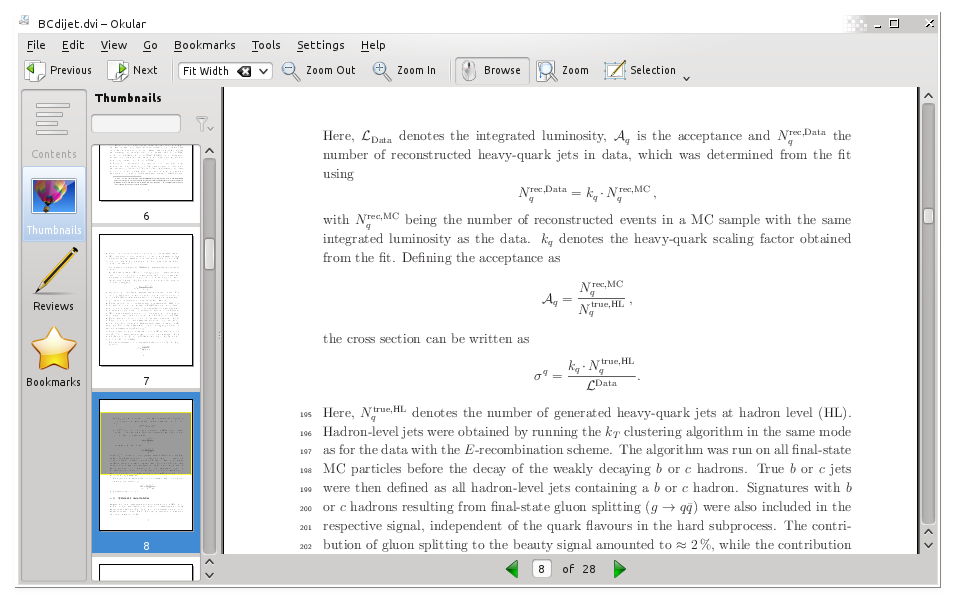
\includegraphics[width=7cm]{BCDijet} &
  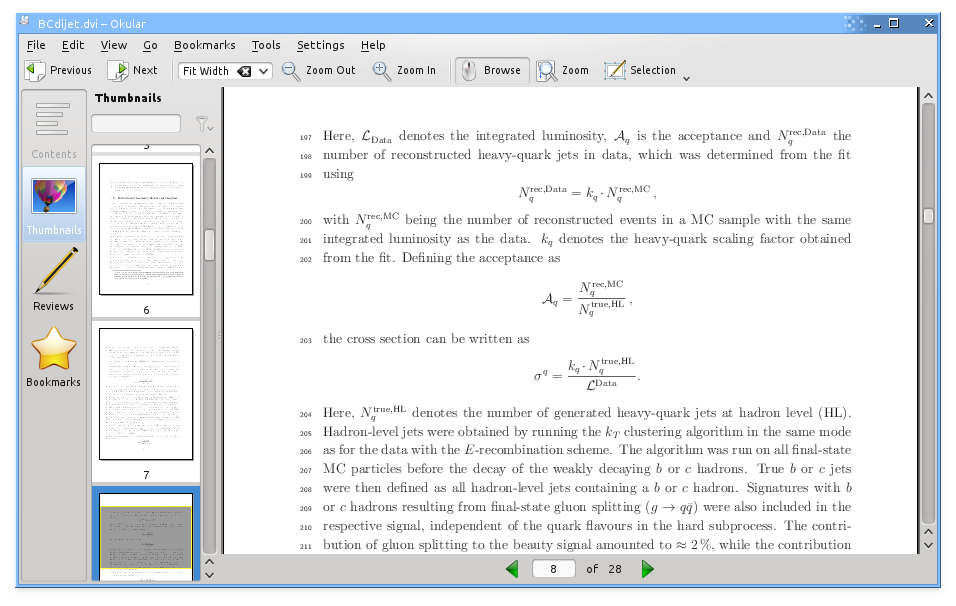
\includegraphics[width=7cm]{BCDijet-linenomath}\\
  (a) & (b)
  \end{tabular}
  \caption{Example of (a) a problem with line numbers and (b) its solution.}
  \label{fig:lineno}
\end{figure}

Such problems are associated with text that is close to math mode
environments. Some of the problems can be solved by using a new
version of the \Package{lineno} package.
However, this only works for \enquote{standard} \LaTeX{}
math environments: \Env{displaymath}, \Env{equation} and \Env{eqnarray}, while it does
not work for recommended \Package{amsmath} environments such as \Env{equation*},
\Env{align(*)} and \Env{alignat(*)}.

The solution is to enclose the equation in \Env{linenomath} environment, e.g.
\begin{verbatim}
The total visible cross section for inclusive heavy-quark jet
production, $\sigma^{q}$, with $q\in\{b,c\}$ is given by
\begin{linenomath}
\begin{equation*}
  \sigma^{q} = \frac{N_{q}^{\text{rec,Data}}}%
    {\mathcal{A}_{q}\cdot\mathcal{L}_{\text{Data}}}.
\end{equation*}
\end{linenomath}
Here, $\mathcal{L}_{\text{Data}}$ denotes the integrated luminosity,
$\mathcal{A}_{q}$ is the acceptance and $N_{q}^{\text{rec,Data}}$ the
number of reconstructed heavy-quark jets in data, which was determined
\end{verbatim}
\noindent
Then the line numbering will be correct, see Fig.~\ref{fig:lineno}b.


%------------------------------------------------------------------------------
\section{Updating \Package{ubonn-thesis}}
\label{sec:tips:update}\index{upadting}\index{ubonn-thesis!updating}
%------------------------------------------------------------------------------

What is the best way to update \Package{ubonn-thesis}? If you are
using Git, then you just need to do an \texttt{git pull}. If you use
a tar file, then you should unpack it and copy over your
\texttt{mythesis} directory tree and any other files you need to the new tree.

Note that when you make a new thesis skeleton (as of version 2.1) the files
\texttt{thesis\_skel/Makefile} and \texttt{ubonn-thesis.sty} 
(and \texttt{ubonn-biblatex.sty}) are copied
to your \texttt{mythesis} directory. If you want to profit from
updates to one of these files, you therefore need to copy the new
version into \texttt{mythesis} again. The advantage of this scheme is
that you can easily check what the differences are before you do the
copy. More importantly, if you have made your own changes to the style
file, it should be relatively easy to merge the two versions. Having
all files in the \texttt{mythesis} subdirectory also makes it much easier
for you to use your own version manager for your thesis.

As a side remark, I would also recommend that you put all Feynman
graphs etc.\ in subdirectories of \texttt{mythesis}. You may have to
change some variables that are set at the beginning of the
\texttt{Makefile} so that this works if you use \Package{feynmf}. If
you use \Package{feynmp} just add \Macro{write18} statements. See
Section~\ref{sec:fig:feynman} for some more details.


%%% Local Variables:
%%% mode: latex
%%% TeX-master: "./thesis_guide"
%%% End:

%\printbibliography[heading=subbibliography]

%------------------------------------------------------------------------------
\chapter{Submitting your thesis}
\label{sec:submit}\index{submit}
%------------------------------------------------------------------------------

\LaTeX{} file: \url{./guide_submit.tex}\\[1ex]
\noindent
Questions often come up when your thesis is finished and now you have
to print it and submit it. Both the
\foreignquote{ngerman}{Promotionsbüro} and the
\foreignquote{ngerman}{Prüfungsamt} have instructions on what you have
to do, but it is sometimes not clear what this means in terms of the
cover pages offered by this thesis framework.

For the printed version of your thesis, you probably want
\Package{hyperref} links and the table of contents to be black. In
order to do this, you should uncomment the \Macro{hypersetup} command
that is in the thesis main file, just after the
\Macro{usepackage}\texttt{\{thesis\_defs\}}.


%------------------------------------------------------------------------------
\section{PhD thesis}
\label{sec:submit:phd}\index{submit!PhD thesis}\index{PhD}

\subsection{Submission}

\begin{enumerate}
\item Use the file \texttt{PhD\_Submit\_Title.tex} for the title
  pages. 
  This is selected by passing the options \Option{PhD, Submit}.
  to the \Macro{documentclass} or the \Package{ubonn-thesis} package.
  Leave the \foreignquote{ngerman}{Tag der Promotion} and
  \foreignquote{ngerman}{Erscheinungsjahr} blank.
\item You are required to also submit a CV\index{CV} and a summary of your
  thesis. A skeleton CV is provided as the file
  \texttt{thesis\_cv.tex} which you then include at the end of your
  thesis. The summary should also be printed separately.
\item You have to print and bind five copies of your thesis for the
  \foreignlanguage{ngerman}{Promotionsbüro}. Nowadays these are
  usually in colour.
\item The first and second referees for your thesis often like to also
  have an extra copy of the thesis so that they can make comments when they read
  your thesis -- ask them if they want one. You can usually save the
  institute some money and print these copies in black \& white.
\end{enumerate}


\subsection{Printing the final version}

\begin{enumerate}
\item Use the file \texttt{PhD\_Final\_Title.tex} for the title page.
  This is selected by passing the options \Option{PhD, Final}.
  to the \Macro{documentclass} or the \Package{ubonn-thesis} package.
\item Do not include your CV.
\item There are probably some small corrections you or the referees
  found during the time between submission and your examination. These
  should be corrected before you submit your thesis to the university
  library (ULB).\index{ULB}\index{university library}\index{library!university}
\item Almost everyone submits their thesis electronically to the
  ULB. You still have to print two copies for them as well.\footnote{%
  This used to be five, but has recently (2015) been reduced.}
  The ULB is quite strict on the quality of the binding etc. The university
  print shop is not able to fulfil the requirements, so you have to print
  these versions externally. When you do this do not forget to
  uncomment the \Macro{hypersetup} command as mentioned above, if you
  want to print them in colour.
\item The department
  library\index{department library}\index{library!department} (in the Physikalisches
  Institut) needs seven printed copies with the file
  \texttt{PhD\_Cover.tex} as the cover and
  \texttt{PhD\_Final\_Title.tex} for the title pages.
  These are selected by passing the options \Option{PhD, PILibrary}
  to the \Macro{documentclass} or the \Package{ubonn-thesis} package.
  You have to get
  the \enquote{BONN-IR-YYYY-nnn} number from the librarian. You
  should also include an abstract (in English) on the cover page. You
  can also use this abstract when you submit your thesis
  electronically to the ULB.
\item The department library version of the thesis is the one that you usually print if
  you need extra copies for your experiment or research group.
\end{enumerate}

Note that when you want to get your degree certificate, you will get
some forms from the \foreignlanguage{ngerman}{Promotionsbüro} that have
to fill out. These forms have to be signed by your supervisor. One of
the forms asks you if you have published significant parts of your
thesis elsewhere. This means your actual thesis and not a paper that
uses the results from your thesis. If you submit your thesis
electronically to the ULB, then you should not fill out this form. It
only applies if you actually publish your thesis elsewhere (which is
allowed by the \foreignlanguage{ngerman}{Promotionsordnung}).

%%% Local Variables:
%%% mode: latex
%%% TeX-master: "./PhD_submit"
%%% End:


Appendix~\ref{app:printer} suggests some print shops that can make copies
of your thesis in good enough quality to be accepted by the university
library.


%------------------------------------------------------------------------------
\section{Master/Diplom/Bachelor thesis}
\label{sec:submit:other}\index{submit!MSc thesis}\index{submit!Diplom thesis}\index{submit!BSc thesis}

\subsection{Submission}

\begin{enumerate}
\item Use the file \texttt{Master\_Submit\_Title.tex},\index{MSc}
  \texttt{Diplom\_Submit\_Title.tex}\index{Diplom} or\\
  \texttt{Bachelor\_Title.tex}\index{BSc} for the title pages.
  These are selected by passing one of the options
  \Option{Master}, \Option{Diplom} or \Option{Bachelor}
  to the \Macro{documentclass} or the \Package{ubonn-thesis} package.
  In addition, pass the option \Option{Submit} to 
  to the \Macro{documentclass} or the \Package{ubonn-thesis} package.
\item You have to print and bind three copies of your thesis
  to be submitted to the
  \foreignlanguage{ngerman}{Prüfungsamt}. Nowadays these are usually in
  colour.
\item The first and second referees for your thesis often like to
  have an extra copy of the thesis so that they can make comments when they read
  your thesis -- ask them if they want one. You can usually save the
  institute some money and print these copies in black \& white.
\end{enumerate}

Note that a CV does not have to be included in a Master/Diplom/Bachelor
thesis. This is only needed when you submit a PhD thesis.


\subsection{MSc/Diplom theses for the department library}

\begin{enumerate}
\item Use the file \texttt{Master\_Cover.tex} for the cover and
  \texttt{Master\_Final\_Title.tex}\footnote{Replace Master with Diplom
    as appropriate.} for the title pages.
  These are selected by passing the options \Option{Master, PILibrary}\footnote{%
    or \Option{Diplom, PILibrary}}
  to the \Macro{documentclass} or the \Package{ubonn-thesis} package.
\item There are probably some small corrections you or the referees
  found during the time between submission and the completion of the
  referees' reports and grades. These should be corrected before you
  submit your thesis to the department library.
\item The department
  library\index{department library}\index{library!department} (in the Physikalisches
  Institut) needs 2 printed copies with the file\\
  \texttt{Master\_Cover.tex} as the cover.
  This is selected by passing the options \Option{Master, PILibrary}
  to the \Macro{documentclass} or the \Package{ubonn-thesis} package.
  You have to get
  the \enquote{BONN-IB-YYYY-nnn} number from the librarian. You
  should also include an abstract (in English) on the cover page.
\item This version of the thesis is the one that you usually print if
  you need extra copies for your experiment or research group.
\end{enumerate}


\subsection{BSc theses}

\begin{enumerate}
\item There are probably some small corrections you or the referees
  found during the time between submission and the completion of the
  referees' reports and grades. These should be corrected before you
  print some extra copies of your thesis if your group wants them.
\end{enumerate}

%%% Local Variables:
%%% mode: latex
%%% TeX-master: "./thesis_guide"
%%% End:

%\printbibliography[heading=subbibliography]

% !TeX root = thesis_guide.tex

%==============================================================================
\chapter{Useful packages}
\label{sec:package}
%==============================================================================

\LaTeX{} file: \url{./guide_package.tex}\\[1ex]
\noindent
\LaTeX{} has so many packages that it is often hard to find the
correct or most useful ones. It is also not a good idea to just take
one of your friend's theses and use his/her packages and conventions,
as there is a steady and regular improvement in the packages
available.

This chapter lists some useful packages -- maybe also some that
are not so commonly known. Here I only say what the package is used
for. More detailed instructions on the usage can be found in the
relevant chapters. I first list the packages used in this guide
and then give a bit of information on other packages that may be useful.

From all that I have read, \KOMAScript\index{KOMAScript@\KOMAScript}
seems to be the way to go for the overall classes. I have therefore
based the \Package{ubonn-thesis} style on this. You replace
\Package{article}, \Package{report} and \Package{book} by
\Package{scrartcl}, \Package{scrreprt} and \Package{scrbook}. For
theses I think it is best to use \Package{scrbook}, as this class also
includes the commands \Macro{frontmatter}, \Macro{mainmatter} and
\Macro{backmatter} that set up page numbering etc.\ appropriately.

Please try to use \KOMAScript\ version 3.0 or higher. The
\Macro{KOMAoptions} command is not available in earlier versions, so
you would have to modify the style file.


%------------------------------------------------------------------------------
\section{Layout and language}
\label{sec:package:layout}
%------------------------------------------------------------------------------

There are quite a few packages related to layout and also to handling
of text input and languages. As far as layout goes, \KOMAScript{} has
many options with which you can already do a lot. You can either use
the built-in \Package{typearea} package to do the page layout, which
also includes nice options to allow for the binding, or use the
\Package{geometry} package which also contains more than enough
options. In the past I have used \Package{geometry}, but I also see no
reason not to just use \Package{typearea}. Note that you should not
include the \Package{typearea} package, you should simply set the
options using \Macro{KOMAoptions}.
The packages are listed in Table~\ref{tab:package:layout}.

\begin{table}[htbp]
  \centering
  \begin{tabular}{lp{0.8\textwidth}}
    \toprule
    \Package{geometry} & Provides simple options for page layout such
    as \Option{scale=0.75} to cover 75\% of the page.\\
    \Package{typearea} & Does much the same, but here you specify how
    many elements to split the page into. You do not have to include
    this package explicitly if you use \KOMAScript.\\
    \Package{setspace} & Useful options to change spacing.\\
    \Package{fontenc} & The encoding used for fonts. Recommended is
    \Option{T1}, which is given as an option.\\
    \Package{inputenc} & Use either \Option{utf8} or \Option{latin1} so
    that you can input German letters such as ä, ü and ß directly.\\
    \Package{babel} & Language specific typesetting.\\
    \Package{csquotes} & Package for quoting things using the correct
    language-dependent symbol.\\
    \Package{scrpage2} & Set headers and footer.\\
    \Package{xspace} & Avoid having to put
    \enquote{\texttt{\textbackslash\ }} or
    \enquote{\texttt{\{\}}} after a macro.\\
    \bottomrule
  \end{tabular}
  \caption{Useful packages for layout.}
  \label{tab:package:layout}
\end{table}

%------------------------------------------------------------------------------
\section{Appearance}
\label{sec:package:appearance}
%------------------------------------------------------------------------------

It used to be the case that nearly all \LaTeX{} documents used the
Computer Modern Fonts. That is no longer necessary. There are rather
complete font sets that are also free that you can use instead.
%In this guide I use a combination of \Package{Palatino} and other fonts.
The default font for theses is \Package{txfonts}.
\Package{newtx} is a new version of this package that is available as of \TeXLive 2013.
If you have this package, then I would recommend using it.
Some of the spacings in equations have been improved 
and there is a better balance of the sizes of serif, \textsf{sans serif} and \texttt{typewriter} fonts.
Other fonts that look quite nice (e.g.\ Palatino) can also be used.
The option \Option{palatino} in \Package{ubonn-thesis} can be used to select this.
The option actually selects the font packages \Package{mathpazo}, \Package{courier} and \Package{helvet}.
Another alternative is a package such as \Package{pxfonts} 
to get both text and math fonts in the same style. 
Some examples of other possible font packages are given in the style file.
As mentioned above, certain fonts can be selected directly via options:
\Option{txfonts}, \Option{newtx} or \Option{palatino}.

Commonly used packages associated with fonts, tables and
figures are listed in Table~\ref{tab:package:appearance}.

\begin{table}[htbp]
  \centering
  \begin{tabular}{lp{0.75\textwidth}}
    \toprule
    \Package{siunitx} & Typeset units properly with correct spacing.\\
    \Package{graphicx} & The package to use for including graphics.\\
    \Package{rotating} & Package to use for rotating tables etc. The
      \Macro{includegraphics} command can rotate figures directly.\\
    \Package{array} & Adds extra column formatting capabilities.\\
    \Package{xtab} & Can produce tables that extend over more than one page.\\
    \Package{booktabs} & Help for producing nicer tables.\\
    \Package{amsmath}, \Package{amssymb} & Extra math commands and symbols from AMS.\\
    \Package{hepnicenames} & A somewhat restricted list of predefined elementary particles.\\
    \Package{heppennames} & A more complete list of predefined elementary particles.
      Note that \Package{hepnicenames} also loads \Package{heppennames}.
      The packages are based on \Package{hepparticles}, which you can use to define further particles.\\
    \Package{mhchem} & Nice package for typesetting chemical elements correctly.\\
    \Package{xfrac} & Some more options for typesetting fractions.\\
    \Package{xcolor} & Add colour commands.\\
    \Package{titlesec} & Change the appearance of chapter and section headings. 
      See below for more information.\\
    \bottomrule
  \end{tabular}
  \caption{Useful packages for appearance.}
  \label{tab:package:appearance}
\end{table}

As alternatives to \Package{xtab}, one can also use
\Package{supertabular} or \Package{longtable}. 
All these packages also have the advantage that you
can specify header and footer text.
If you use the \Env{mpxtabuar} environment from \Package{xtab} 
you can include footnotes in a table.
See the \Package{xtab} documentation for more details.
It is probably best to only use one of these three packages to avoid conflicts.

Use of the \Package{titlesec} package gives a warning when using \KOMAScript{}; hence
as of version 3.0 the chapter title formatting is done by hand in \Package{ubonn-thesis}.
You can switch back to using \Package{titlesec} by giving the option \Option{titlesec}.


%------------------------------------------------------------------------------
\section{Other packages}
\label{sec:package:other}
%------------------------------------------------------------------------------

Some other useful packages, some of which are included in
\texttt{ubonn-thesis.sty} are listed in
Table~\ref{tab:package:other1}.

\begin{table}[htbp]
  \centering
  \begin{tabular}{lp{0.8\textwidth}}
    \toprule
    \Package{ifthen} & Provides the \Macro{ifthenelse} command.\\
    \Package{IEEEtrantools} & Contains useful environments for multiline equations.\\
    \Package{feynmp} & Draw Feynman graphs with Metapost.\\
    \Package{axodraw} & Draw Feynman graphs.\\
    \Package{tikz} & General drawing package that can also be used for Feynman graphs.\\
    \Package{standalone} & Allows you to have a document that you can
    directly compile for each figure and also input to another document.\\
    \Package{hyperref} & Adds \Macro{url} command as well as ability
    to click on entries on table of contents etc.\\
    \Package{background} & Allows you to add things like DRAFT across the whole document page.\\
    \Package{subfiles} & Provides a nice alternative to
    \Macro{include}.\\
    \Package{subcaption} & An newer alternative to \Package{subfig}.\\
    \Package{tabularx} & Allows fixed table width with flexible column widths.\\
    \Package{floatrow} & Add ability to define own floats.\\
    \Package{physics} & Some useful extra maths commands, especially for differentials.\\
    \Package{commath} & Some useful extra maths commands -- has not been updated for a while.\\
    \Package{skmath} & More maths commands that could be useful.\\
    \Package{adjustbox} & Add much more sophisticated clipping
    capabilities than offered by \Package{graphicx}.\\
    \Package{wrapfig} & Allow text to flow around figures.\\
    \Package{floatflt} & Similar capabilities to \Package{wrapfig} -- allow text to flow around figures.\\
    \Package{glossaries} & Provide commands for creating a glossary.
      This is intended to replace the \Package{glossary} package.\\
    \Package{dcolumn} & Very helpful for lining up columns on character strings such as a decimal point.
      \Package{siunitx} offers similar and better functionality.\\
    \Package{refcheck} & Check whether labels are used, i.e.\ if figures and tables are actually referenced.\\
    \bottomrule
  \end{tabular}
  \caption{Other useful packages.}
  \label{tab:package:other1}
\end{table}

While the \Package{amsmath} package solves many problems that occur if
you just use the normal \LaTeX{} math mode commands, there are some
things that are not so nice with long and complicated multiline
equations. 
\Package{IEEEtrantools}, in particular the \Env{IEEEeqnarray} environment, can help here.
See Ref.~\cite{lshort} or the package documentation for more details.

\Package{standalone} is both a package and a document class. It is
available from \TeXLive 2012 onwards. It allows you to have a
standalone document for a \Package{tikz} or \Package{feynmf} figure
and also input this file into another document. If you run PDF\LaTeX\
on the file it also automatically crops the resulting picture. This is
one of those packages where you think \enquote{Why didn't someone
  create this years ago?}. The \Package{tikz} figures included in this
guide make use of it.

I do not recommend the \Package{subfiles} package by default as it is not
included in \TeXLive by default. Have a look at
\url{http://en.wikibooks.org/wiki/LaTeX/General_Guidelines} for
example for more information. If you want to use the package you have
to download it and install for yourself. You can do much the same
thing using AUCTeX inside \texttt{emacs}.

The packages \Package{physics}, \Package{commath} and \Package{skmath} provide some additional maths commands.
Differentials etc.\ are particularly useful.
The \Package{physics} package contains a lot of nice and flexible definitions and also handles the spacing around things like $\dd{x}$ well,
if you use the \verb|\dd{x}| construction.
The \Package{commath} package has not been updated for a while.
\Package{skmath} does quite a lot more then \Package{commath} and even modifies/enhances some standard commands.

\begin{sloppypar}
Note that there is a conflict if you use \Package{refcheck}, \Package{subcaption} and \Package{hyperref} together.
See \url{http://tex.stackexchange.com/questions/273970/conflict-refcheck-subcaption-packages-for-label-with-underscores} for a workaround.
\end{sloppypar}

It is often useful to indicate whether your thesis is in the draft stage.\index{draft}
The thesis skeleton uses the package \Package{background} for this.
It is only available as of \TeXLive 2011.
Hence \enquote{Draft} is instead put in the heading for older versions.
As an alternative, you can try the package \Package{draftwatermark}.\footnote{%
\Package{draftwatermark} needs \Macro{unitlength} to be set to \SI{1}{pt}.
This is not the default setting in \Package{ubonn-thesis}.
The 2009 thesis skeleton contains \Macro{setlength\{\Macro{unitlength\}\{1pt\}}} (commented out).
Given that this is a global setting, neither it nor \Package{draftwatermark} are included by default.}

A list of other packages that are commonly used is given in
Table~\ref{tab:package:other2}. They are not
included in the list above, because they are either not really needed
or have been superseded by other packages.

\begin{table}[htbp]
  \centering
  \begin{tabular}{lp{0.8\textwidth}}
    \toprule
    \Package{hepunits} & Typeset units properly with correct spacing.\\
    \Package{units} & Typeset units properly with correct spacing.\\
    \Package{SIunits} & Typeset units properly with correct spacing.
      \Package{hepunits} uses this package, so it does not need to be added explicitly\\
    \Package{fancyhdr} & As the name suggests, do your own header and footer configuration.
      Within \KOMAScript{} it is recommended to use \Package{scrpage2} instead.\\
    \Package{feynmf} & Draw Feynman graphs with Metafont.\\
    \Package{draftwatermark} & Another package that allows you to add DRAFT to the background each page.\\
    \Package{subfig} & As the name suggests make sub-figures and add
    separate captions for them. \emph{This package has apparently been
      deprecated.}\\
    \Package{subfigure} & As the name suggests make sub-figures and add
    separate captions for them. \emph{This package is deprecated.}\\
    \Package{color} & Add colour commands -- \Package{xcolor} is
    needed to colour boxes around links.\\
    \Package{float} & As far as I can tell \Package{floatflt} offers more options.\\
    \Package{caption} & Much more control on captions -- as
    \KOMAScript{} also has many options, not sure this is necessary.\\
    \Package{ziffer} & Spacing with a comma as decimal separator is
    correct.\\
    \Package{nomencl} & Another package for creating a glossary.\\
    \Package{fncychap} & Another package for changing the style of the
    chapter heading.\\
    \Package{quotchap} & Another package for changing the style of the
    chapter heading.\\
    \bottomrule
  \end{tabular}
  \caption{Other packages that are often used, but I have already
    given alternatives.}
  \label{tab:package:other2}
\end{table}

As indicated, the \Package{ziffer} package is advertised as providing
the correct spacing after a comma in math mode if you use the comma as
the decimal separator. Compare $2,5$ with 2,5 and $2{,}5$. The first
spacing is wrong. If you use the \Package{ziffer} package it will be
correct. However, it does seem to conflict with the use of the
\Package{dcolumn} package, so I cannot compile this guide
if \Package{ziffer} is included. Some  workarounds are discussed in
Section~\ref{sec:layout:german}. In addition, the \Package{siunitx}
package contains the same functionality, which can simply be steered
by changing the document language, as discussed in
Section~\ref{sec:table:siunitx}. Hence, \Package{ziffer} is not really
needed anymore.

%\printbibliography[heading=subbibliography]

%==============================================================================
\chapter{Figures}
\label{sec:fig}\index{figures}
%==============================================================================

\LaTeX{} file: \url{./guide_figs.tex}\\[1ex]
\noindent
This chapter discusses what you need to know to include graphics in
your thesis. The basic command to use is \Macro{includegraphics}.

I recently found a pretty complete guide (in German) called \texttt{l2piqfaq}
which can be obtained from
\url{http://www.ctan.org/tex-archive/info/l2picfaq/german}. It contains
a lot of detailed information and tricks.

The chapter also contains some suggestions as to how to create Feynman
graphs with a number of different packages.

%------------------------------------------------------------------------------
\section{Simple figures}
\label{sec:fig:simple}
%------------------------------------------------------------------------------

A simple figure and its associated caption is straightforward to
include. For example, the layout of the LHC and its experiments is
shown in Fig.~\ref{fig:LHC}.

\begin{figure}[htbp]
  \centering
  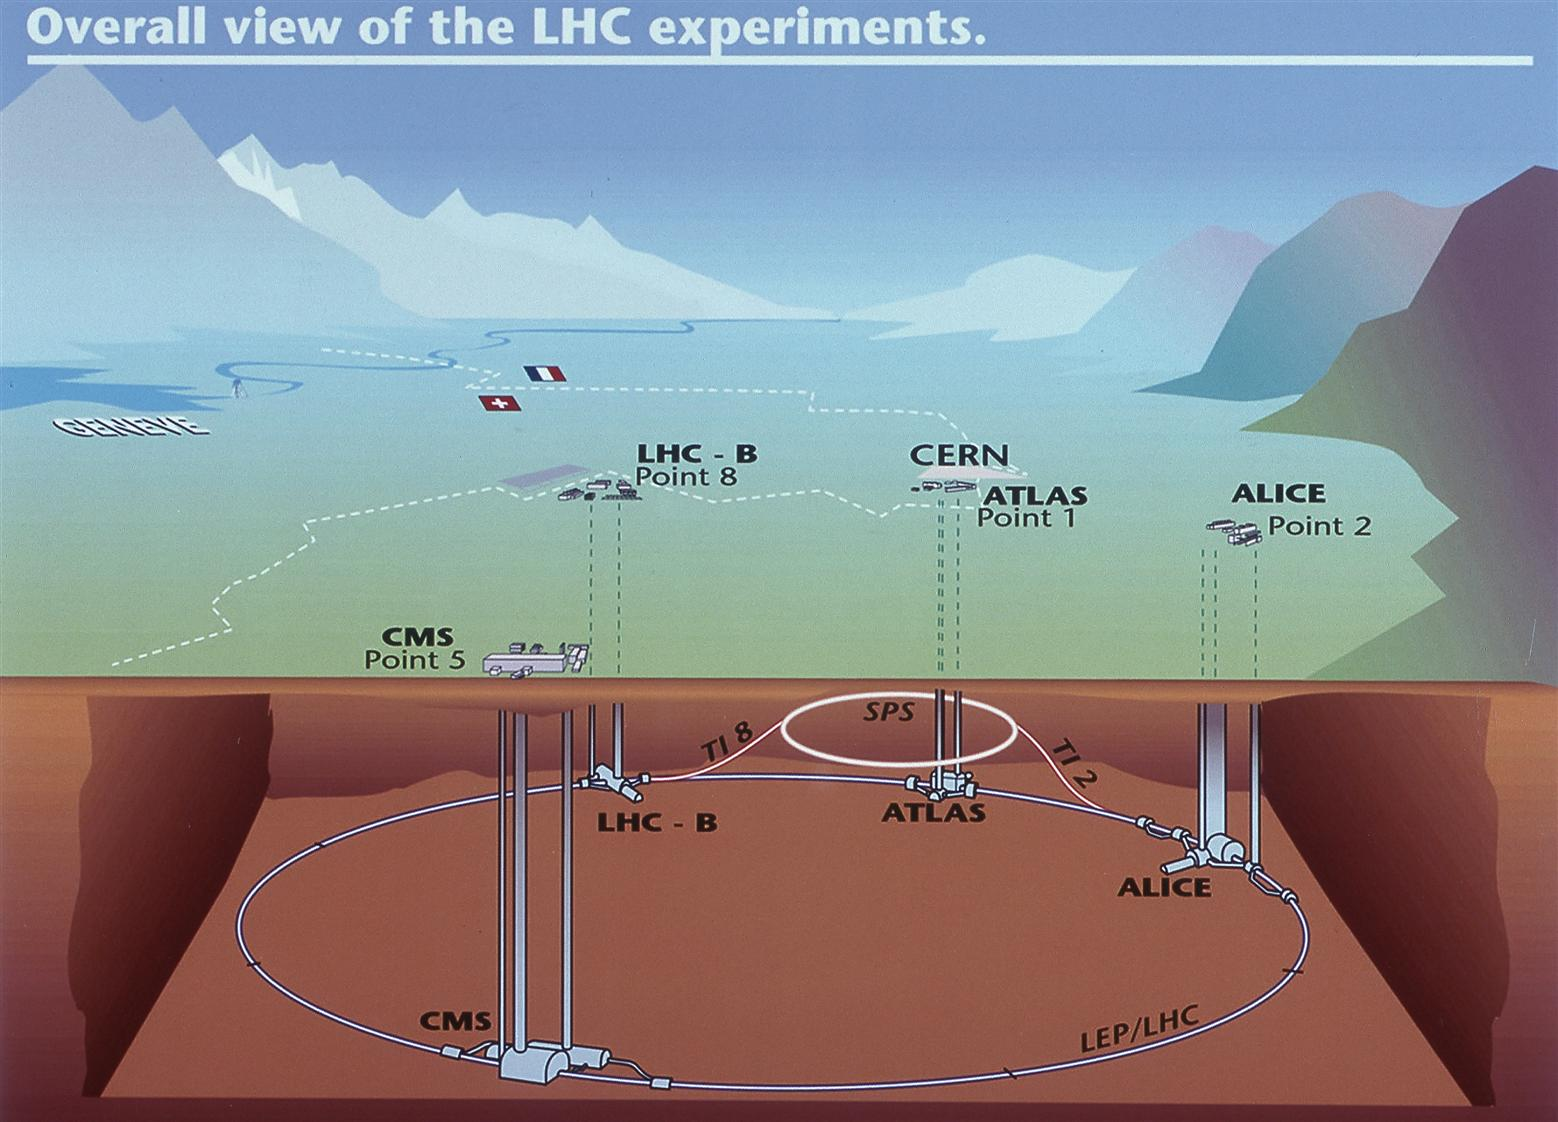
\includegraphics[width=\figwidth]{CERN_all-experiments}
  \caption[Sketch of the LHC ring, the position of the experiments and
  the surrounding countryside.]{Sketch of the LHC ring, the position
    of the experiments and the surrounding countryside. The four big
    LHC experiments are indicated. The location of the injection lines
    and the SPS are also shown.}
  \label{fig:LHC}
\end{figure}

Note the use of \Macro{centering} rather than the environment
\BegEnv{center} \ldots \EndEnv{center} to centre the figure. This
avoid adding extra vertical space. It is also important that the
\Macro{label} be either inside the caption or after it. If your
caption is more than 1 (or 2) lines, you should also give a short form
that will appear in the ``List of Figures''.

One tricky question is how to best format the caption. This document
uses a smaller font and no extra indentation. Often italics are
used. I dislike this, as symbols are then formatted in different ways
in the main text and in the caption. One can also reduce the width of
the caption. The font for the caption can be specified using the
\Macro{setkomafont}\texttt{\{caption\}} command. You can specify how
to label the figure by changing the \Macro{figureformat} command. The
captions in this document follow the standard \KOMAScript{}
convention: if they are one line long they are centred; if they are
longer they are left-adjusted. If you want them all to be
left-adjusted set the \Option{KOMAoptions} \Option{caption=nooneline}
in \texttt{ubonn-thesis.sty}. Some examples of the possibilities are
included in the style file.

Another thing to consider is whether the text should be indented or
not. For short captions, indentation is OK. I do not think it looks
good for long captions. Hence the style file sets
\Macro{setcapindent}\texttt{\{0pt\}}.

%------------------------------------------------------------------------------
\section{Fancier figures}
\label{sec:fig:fancy}\index{figures!multiple}
%------------------------------------------------------------------------------

Life gets more complicated if you want to include several plots in
one figure, if you want the caption next to the figure, or if you want
the text to \enquote{flow} around the figure. For the first case I like to
use the \Env{tabular} environment to place the plots, although
there are other ways of doing it.

Another very nice way to add (a), (b) etc. to the figure is to use the
\Macro{put} command. This has the big advantage that you can display
the letters in the figure without actually having to add them to the
EPS/PDF file. Figure~\ref{fig:letters1} shows how this is done. Note
that the origin of the coordinate system is the bottom right-hand
corner of the file that you have included (assuming that the
\Macro{put} command comes just after the \Macro{includegraphics}).
The units for the \Macro{put} command are set with the
\Macro{setlength}\texttt{\{\textbackslash unitlength\}} command, which
is by default set to \SI{1}{\mm} in \texttt{ubonn-thesis.sty}. The
same units are also used for Feynman graphs made with the
\Package{feynmf} and/or \Package{feynmp} package -- see
Section~\ref{sec:fig:feynman:feynmf}.

\begin{figure}[htbp]
  \centering
  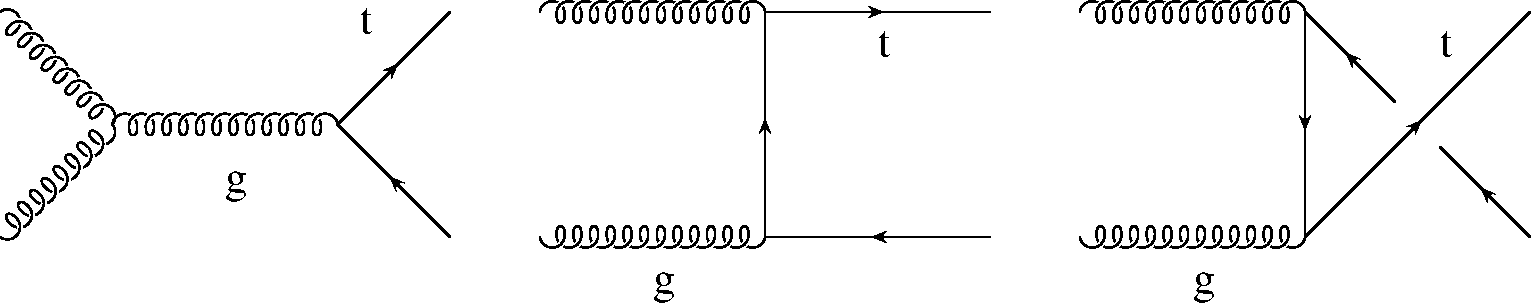
\includegraphics[width=\figwidth]{gg_tt}
  \put(-130,14){(a)}
  \put(-80,14){(b)}
  \put(-35,14){(c)}
  \caption{Adding letters to figures with \Macro{put}.}
  \label{fig:letters1}
\end{figure}

Another way of achieving the same thing, but this time with the letter
outside the figure is to use \Env{tabular}. An example of this is
shown in Fig.~\ref{fig:letters2}.

\begin{figure}[htbp]
  \centering
  \begin{tabular}{@{\hspace*{0.15\figwidth}}p{0.33\figwidth}p{0.33\figwidth}l}
    \multicolumn{3}{c}{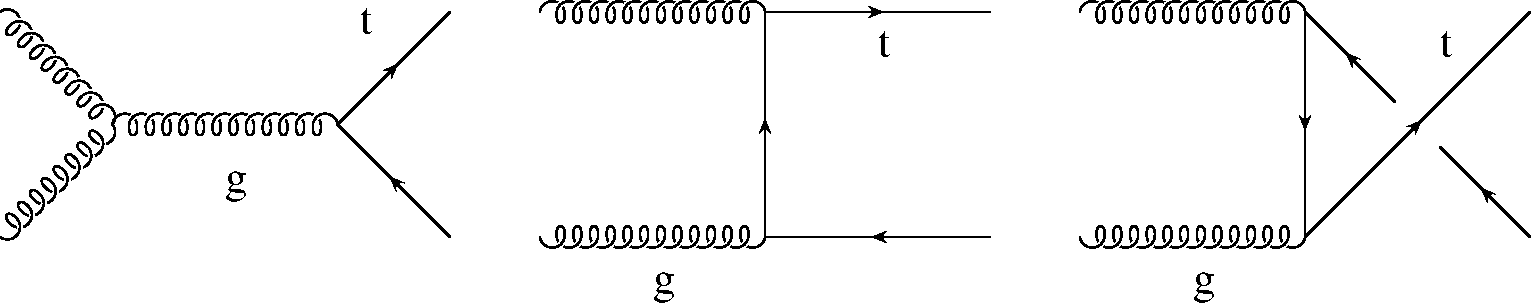
\includegraphics[width=\figwidth]{gg_tt}}\\
    (a) & (b) & (c)
  \end{tabular}
  \caption{Adding letters to figures with \Env{tabular}.}
  \label{fig:letters2}
\end{figure}

If you want to save space it is sometimes nice to put the caption next
to the figure. While packages exist to do this, \KOMAScript{} has its
own built-in \Env{captionbeside} environment. The placement option comes
after the caption itself and can be one of:
\begin{description}\setlength{\parskip}{0pt}
\item[l] Left of figure
\item[r] Right of figure
\item[i] Inner margin in two-sided layout
\item[o] Outer margin in two-sided layout
\end{description}
Note that this is an environment rather than a macro and that the
figure itself is inside the environment. Also the placement does not
seem to work exactly how it is advertised in the manual. I set the
width equal to \Macro{figwidth} and then the offset to \texttt{-\Macro*{figwidth}}.

\begin{figure}[htbp]
  \centering
  \begin{captionbeside}{A small figure with a simple caption beside it.}[i][\figwidth][-\figwidth]
    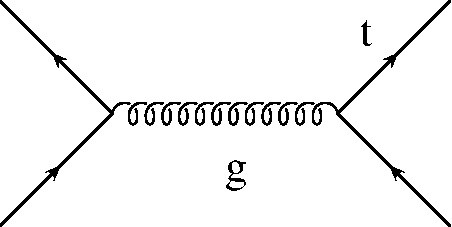
\includegraphics[width=0.3\textwidth]{qq_tt}
  \end{captionbeside}
  \label{fig:qqtt}
\end{figure}

If you want different (partial) captions for a figure then the
\Package{subfig} package used to be the way to go. 
An alternative, and successor, to \Package{subfig} is
\Package{subcaption}. It works in much the same way as
\Package{subfig}. A nice tutorial on its use can be found in
\url{http://www.peteryu.ca/tutorials/publishing/latex_captions}.
An example of its use can be seen in Fig.~\ref{fig:nccc}.
The \LaTeX\ file \texttt{guide\_figs.tex} contains examples for both \Package{subfig} and 
\Package{subcaption}, as the way \Package{subcaption} should be used was
different for \TeXLive 2011 and earlier.
You can see how to reference
the different parts of the figure in Section~\ref{sec:fig:feynman}. If
you want the captions of the sub-figures to also appear in the
\enquote{List of Figures} you should include the package with the
option \Option{lofdepth}. For tables use the option \Option{lotdepth}.


\ifthenelse{\texlive < 2012}{%
\begin{figure}[htbp]
  \centering
  \subfloat[NC scattering]{%
    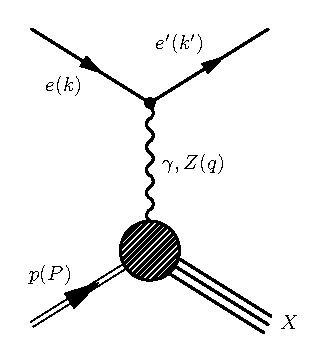
\includegraphics[width=0.5\figwidth]{ep_nc}
    \label{fig:nccc-nc}
  }
  \qquad
  \subfloat[CC scattering]{%
    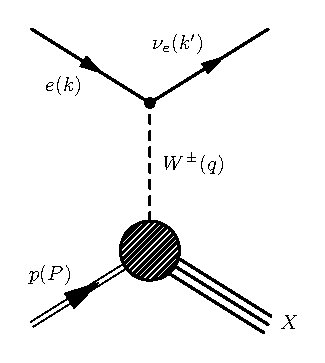
\includegraphics[width=0.5\figwidth]{ep_cc}
    \label{fig:nccc-cc}
  }
  \caption{Processes in $ep$ scattering.}
  \label{fig:nccc}
\end{figure}
}{%
\begin{figure}[htbp]
  \centering
  \begin{subfigure}[b]{0.5\figwidth}
    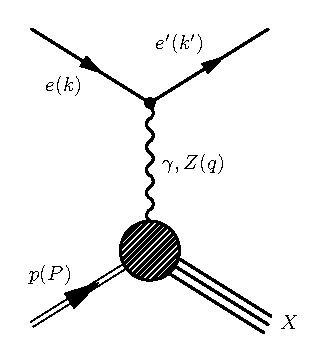
\includegraphics[width=0.5\figwidth]{ep_nc}
    \caption{NC scattering}\label{fig:nccc-nc}
  \end{subfigure}
  \qquad
  \begin{subfigure}[b]{0.5\figwidth}
    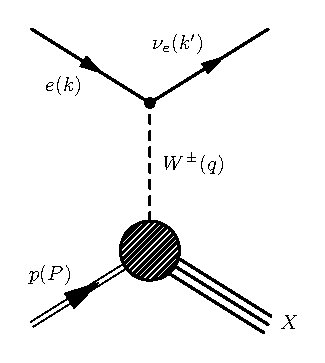
\includegraphics[width=0.5\figwidth]{ep_cc}
    \caption{CC scattering}\label{fig:nccc-cc}
  \end{subfigure}
  \caption{Processes in $ep$ scattering.}
  \label{fig:nccc}
\end{figure}
}

If you run out of space (applies more often to proceedings than to
theses) you can use the \Package{wrapfig} package.


%------------------------------------------------------------------------------
\section{Figure Formats}
\label{sec:fig:formats}\index{figures~formats}
%------------------------------------------------------------------------------

If you use plain \LaTeX, you are pretty much stuck with encapsulated
postscript (EPS) as your figure format. If you use PDF\LaTeX, then you
have much more freedom, with the notable exception that you cannot
include EPS files!\footnote{%
This restriction has finally been lifted with \TeXLive 2011. It
simply converts the EPS files to PDF inline.}
I would still recommend that you always try to use
a vector graphic format. What usually works well is to either create
PDF directly or to create EPS and then convert from EPS to PDF.

The tool I use for conversion is \texttt{epstopdf}. Occasionally this
fails; in that case \texttt{eps2eps} can help. It is important that
the bounding box is set correctly in the EPS file before you run
\texttt{epstopdf}.

If these fail, you can try the \texttt{convert} command which is part
of \texttt{ImageMagick}. A more powerful tool is \texttt{inkscape}
which is a successor to \texttt{xfig}. Professionals use Adobe Illustrator!


%------------------------------------------------------------------------------
\section{\TikZ and PGF}
\label{sec:fig:tikz}\index{TikZ@\TikZ}
%------------------------------------------------------------------------------

\Package{pgfplots} and \Package{tikz} are packages to help with
creating graphics \enquote{inline}. For 3D figures you also need
\Package{tikz-3dplot}. PGF is the backend, while \TikZ is what the
user interacts with directly. The manual contains all the information
you should need, but is 726 pages long at the last count, so it may
not to be too easy to find what you want!

I do not have much experience with using these packages so far, so
this section will certainly not cover all possibilities. There may
also be better ways of doing things than I illustrate here. The
examples I give come from Andrii Verbytskyi or are adapted from
questions and answers found on
\url{http://tex.stackexchange.com/}. The examples included in this
guide and a few more are collected in the \texttt{tikz}
subdirectory. Note that some of the examples only work with \TeXLive
2011 and later. This is indicated in the file. I also did not manage
to compile the guide without errors when including \Package{tikz} with
\TeXLive 2009, so some of the figures may be missing if you compile
your own version of the guide with \TeXLive 2009.

\TikZ is not included by default in a new skeleton thesis. See the
commented out packages in a new thesis skeleton or
\texttt{thesis\_guide.tex} for the packages and \TikZ libraries that
you should include if you want to use it.

You often want to include a figure of your experiment's coordinate
system in your thesis. One way to do this is illustrated in
Fig.~\ref{fig:tikz:coord}.

\begin{figure}[htbp]
  \centering
  \ifthenelse {\texlive < 2012} {%
    \fbox{\parbox[c]{0.8\textwidth}{%
    Sorry, \Package{tikz-3dplots} is not available in \TeXLive 2009 and
    earlier. See the file \texttt{./tikz/zeus\_coords.tex}.}
    This example also does not work with \TeXLive 2011.}
  }{%
    % This figure only works with \TeXLive 2011 and later.
% The ZEUS coordinate system
\documentclass{standalone}

\usepackage{siunitx}
\usepackage{tikz}
\usepackage{tikz-3dplot}
\usepackage{pgfplots}
\usetikzlibrary{positioning,shapes,arrows}
\usetikzlibrary{decorations.pathmorphing}
\usetikzlibrary{decorations.markings}

\begin{document}
% \setstretch{1.0}
\tdplotsetmaincoords{60}{160}
\begin{tikzpicture}[tdplot_main_coords]
  \draw[thick,->] (-1,0,0) -- (3,0,0) node[anchor=north east]{$z$};
  \draw[thick,->] (0,0,0)  -- (0,4,0) node[anchor=north west]{$x$};
  \draw[thick,->] (0,0,0)  -- (0,0,4) node[anchor=south]{$y$};
  \tdplotdefinepoints(0,0,0)(5,0,0)(3,3,3)
  \draw[dashed,black]  (\tdplotbx,\tdplotby,\tdplotbz) -- (\tdplotvertexx,\tdplotvertexy,\tdplotvertexz);
  \tdplotdrawpolytopearc[thick]{1}{anchor=east}{$\theta$}
  \tdplotdefinepoints(0,0,0)(0,5,0)(0,5,5)
  \draw[dashed,black]  (\tdplotbx,\tdplotby,\tdplotbz) -- (\tdplotvertexx,\tdplotvertexy,\tdplotvertexz);
  \tdplotdrawpolytopearc[thick]{1}{anchor=west}{$\phi$}
  \draw[->,thick,red]  (0,0,0)  -- (3,3,3);
  \draw[black,dashed]  (3,3,3)  -- (0,3,3);
  \draw[blue,thick,->] (6,0,0)  -- (4,0,0)  node[anchor=south east]{$e$};
  \draw[blue,thick,->] (-4,0,0) -- (-2,0,0) node[anchor=south west]{$p$};
\end{tikzpicture}
\end{document}

  }
  \caption{The ZEUS coordinate system.}
  \label{fig:tikz:coord}
\end{figure}

It is also possible to make flow charts with \TikZ. This is
illustrated in Fig.~\ref{fig:tikz:flow}.

\begin{figure}[htbp]
  \centering
  \ifthenelse {\texlive < 2011} {%
    \fbox{\parbox[c]{0.8\textwidth}{%
        Error messages appear when trying to compile the guide with
        \Package{tikz} and \TeXLive 2009, so the figure is not included.
        See the file \texttt{../tikz/zeus\_reconstruction.tex}.}}
  }{%
    \documentclass{standalone}

\usepackage{siunitx}
\usepackage{tikz}
\usepackage{tikz-3dplot}
\usepackage{pgfplots}
\usetikzlibrary{positioning,shapes,arrows}
\usetikzlibrary{decorations.pathmorphing}
\usetikzlibrary{decorations.markings}

\begin{document}
% \setstretch{1.0}
\tikzstyle{decision} = [diamond, draw, fill=blue!20,
    text width=4.5em, text badly centered, node distance=3cm, inner sep=0pt]
\tikzstyle{block} = [rectangle, draw, fill=blue!20,
    text width=5em, text centered, rounded corners, minimum height=4em]
\tikzstyle{block2} = [rectangle, draw, fill=blue!20,
    text width=5em, text centered, rounded corners, minimum height=4em, minimum width=10em]
\tikzstyle{line} = [draw, -latex']
\tikzstyle{cloud} = [draw, ellipse,fill=red!20, node distance=3cm,
minimum height=2em]
\begin{tikzpicture}
  [scale=1.68]
  \clip (-6.0cm,0.6cm) rectangle (2.6cm,-9.6cm);
  \node[draw,    ellipse,fill=red!20,   text centered,minimum height=16mm, text width=24mm](Generator) at (-1cm,0mm){Event generator};
  \node[draw,    ellipse,fill=red!20,   text centered,minimum height=16mm, text width=24mm](Collision) at (0.8cm,0mm){Collision};
  \node[rectangle, draw, fill=blue!20,  text width=22mm, minimum height=12mm, text centered, rounded corners](MOZART)    at (-1cm,-1.5cm){MOZART};
  \node[rectangle, draw, fill=blue!20,  text width=22mm, minimum height=12mm, text centered, rounded corners](Detector)  at (0.8cm, -1.5cm){Detector};
  \node[rectangle, draw, fill=blue!20,  text width=22mm, minimum height=12mm, text centered, rounded corners](ZGANA)     at (-1cm,-3.0cm){ZGANA};
  \node[rectangle, draw, fill=blue!20,  text width=22mm, minimum height=12mm, text centered, rounded corners](Trigger)   at (0.8cm, -3.0cm){Trigger};
  \node[rectangle, draw, fill=white!20, text width=22mm, minimum height=12mm, text centered, rounded corners](Rejection) at (1.8cm, -4.5cm){Event rejection};
  \node[rectangle, draw, fill=blue!20,  text width=22mm, minimum height=12mm, text centered, rounded corners](ZEPHYR)    at (-0.1cm, -4.5cm){ZEPHYR};
  \node[rectangle, draw, fill=blue!20,  text width=22mm, minimum height=12mm, text centered, rounded corners](Orange)    at (-0.1cm, -6.0cm){ORANGE and PHANTOM};
  \node[rectangle, draw, fill=white!20, text width=22mm, minimum height=12mm, text centered, rounded corners](NTP)       at (-0.1cm, -7.5cm){NTuples};
  \node[rectangle, draw, fill=white!20, text width=22mm, minimum height=12mm, text centered, rounded corners](AN)        at (-0.1cm, -9.0cm){Analysis};


  \node [draw, ellipse,fill=red!20,    minimum height=3mm,  text centered, text width=45.0mm]  (MCC)   at (-4cm,-1.15cm) {MOZART control cards};
  \node [draw, ellipse,fill=red!20,    minimum height=3mm,  text centered, text width=45.0mm]  (MGF)   at (-4cm,-1.65cm) {MOZART GAFs};

  \node [draw, ellipse,fill=red!20,    minimum height=3mm,  text centered, text width=45.0mm]  (ZCC)   at (-4cm,-2.65cm) {ZGANA control cards};
  \node [draw, ellipse,fill=red!20,    minimum height=3mm,  text centered, text width=45.0mm]  (ZGF)   at (-4cm,-3.15cm) {ZGANA GAFs};


  \node [draw, ellipse,fill=red!20,    minimum height=3mm,  text centered, text width=45.0mm]  (ZPCC)  at (-4cm,-4.15cm) {ZEPHYR control cards};
  \node [draw, ellipse,fill=red!20,    minimum height=3mm,  text centered, text width=45.0mm]  (ZPGF)  at (-4cm,-4.65cm) {ZEPHYR GAFs};

  \node [draw, ellipse,fill=red!20,    minimum height=3mm,  text centered, text width=45.0mm]  (OCC)   at (-4cm,-5.65cm) {ORANGE control cards};
  \node [draw, ellipse,fill=red!20,    minimum height=3mm,  text centered, text width=45.0mm]  (OGF)   at (-4cm,-6.15cm) {ORANGE GAFs};


  \path [line,dashed] (Generator) -- (MOZART);
  \path [line,dashed] (Collision) -- (Detector);


  \path [line,dashed] (MCC) -- (MOZART);
  \path [line,dashed] (MGF) -- (MOZART);


  \path [line,dashed] (ZCC) -- (ZGANA);
  \path [line,dashed] (ZGF) -- (ZGANA);

  \path [line,dashed] (ZPCC) -- (ZEPHYR);
  \path [line,dashed] (ZPGF) -- (ZEPHYR);

  \path [line,dashed] (OCC) -- (Orange);
  \path [line,dashed] (OGF) -- (Orange);


  \path [line] (MOZART) -- (ZGANA);
  \path [line]  (ZGANA) -- (ZEPHYR);

  \path [line] (Detector) -- (Trigger);
  \path [line]  (Trigger) -- (ZEPHYR);
  \path [line]  (Trigger) -- (Rejection);

  \path [line]  (ZEPHYR) -- (Orange);
  \path [line]  (Orange) -- (NTP);
  \path [line]  (NTP) -- (AN);
\end{tikzpicture}
\end{document}

  }
  \caption[Event reconstruction and simulation in ZEUS]{Event reconstruction and simulation in ZEUS.}
  \label{fig:tikz:flow}
\end{figure}

There are many more possibilities,
including plots which you would otherwise make with \texttt{root} or
some other graphics program. An example plot showing the effect of
systematic variations can be found in App.~\ref{sec:app:tikz}. Making
Feynman graphs with \TikZ is covered in
Section~\ref{sec:fig:feynman:tikz}.


%------------------------------------------------------------------------------
\subsection{\Package{standalone} package and class}
\label{sec:fig:standalone}

The \Package{standalone} package provides a great way of developing
figures in small files and then inputting these files directly,
without making any changes, into your thesis!

It is in fact both a package and a document class. It is
available from \TeXLive 2012 onward. It allows you to have a
standalone document for a \Package{tikz} or \Package{feynmf} figure
and also input this file into another document. If you run PDF\LaTeX\
on the file it also automatically crops the resulting picture. This is
one of those packages where you think \enquote{Why didn't someone
  create this years ago?}. The \TikZ figures that I include in this
guide (see subdirectory \texttt{tikz}) make use of this package. If
you want to use it, make sure that you also include this package in
your thesis.


%------------------------------------------------------------------------------
\section{Feynman graphs}
\label{sec:fig:feynman}\index{figures!Feynman graphs}\index{Feynman graphs}
%------------------------------------------------------------------------------

You have lots of Feynman graphs you want to include, but how do you
generate them? This is another area where most people (including me)
have found one way to do it and never change! I use \texttt{Mn\_Fit},
mainly because I wrote it and therefore know inside out how it
works. Examples can be found on my web page:
\url{http://pi.physik.uni-bonn.de/~brock/feynman}.

Alternatives include \Package{axodraw} and the \Package{feynmf} or
\Package{feynmp} packages.  It is also possible to use
\Package{tikz}. The use of \Package{feynmf} and \Package{feynmp} is
described in Section~\ref{sec:fig:feynman:feynmf}, while a few
examples of usage of \Package{tikz} are given in
Section~\ref{sec:fig:feynman:tikz}. Examples of Feynman graphs made
with \Package{feynmf} and \Package{feynmp} can be found in the
\texttt{feynmf} directory, while those made with \Package{tikz} can
be found in the \texttt{tikz} subdirectory.

Instructions on how to use \Package{axodraw} may come at a later
date -- contributions would be welcome! Several people have claimed
that \texttt{jaxodraw} is the way to go. This is a Java package which
you can download from \url{http://jaxodraw.sourceforge.net/}. It has
a Graphical User Interface (GUI) to \Package{axodraw} and so is simple and
straightforward to use.

This paragraph illustrates how to reference different parts of a
figure that uses the environment \Env{subfigure} from the package \Package{subcaption}.
If you compile the guide with \TeXLive 2011 or earlier the
environment \Env{subcaption} from the package \Package{subfig} is used.
The NC and CC graphs shown in
Fig.~\ref{fig:nccc}, or more accurately in Fig.~\ref{fig:nccc-nc} and
Fig.~\ref{fig:nccc-cc} were made with \Package{feynmp}. Another way of
saying the same thing is that typical Feynman graphs for $ep$
scattering are shown in Fig.~\ref{fig:nccc}, where
\subref{fig:nccc-nc} shows a neutral current and \subref{fig:nccc-cc}
show a charged current process.


%------------------------------------------------------------------------------
\subsection{FeynMF and FeynMP}
\label{sec:fig:feynman:feynmf}\index{feynmf}\index{feynmp}

In order to use \Package{feynmf} or \Package{feynmp}, you have to put
the commands to draw the graph in a \LaTeX{} file and then process
this file with \LaTeX{} and either Metafont or
Metapost.\footnote{\texttt{ubonn-thesis.sty} now includes \Package{feynmp}
  by default for \TeXLive 2011 and later. If you want to use
  \Package{feynmf} instead just change the name.}  You can either make
a separate \LaTeX{} file containing the Feynman graph or include the
commands inside your normal \LaTeX\ file.  Metapost\index{metafont} is
a bit easier to use than Metafont.  You should be able to just run
\texttt{mpost} after \texttt{(pdf)latex} and then run
\texttt{pdflatex} again twice. Note that you have to run
\texttt{mpost} on all the files whose names are defined at the
beginning of the \Env{fmffile} environment. While Metapost works well
as of \TeXLive 2011, I did not get it to work properly with \TeXLive
2009 for unknown reasons.

Metafont\index{metafont} is a bit trickier. On Unix systems the
\texttt{feynmf} perl script exists that runs both \LaTeX{} and
Metafont for you. This will produce a \texttt{dvi} file that you then
then look at or use to make a Postscript/PDF file.

I think a better way to proceed is the following:
\begin{itemize}
\item make a separate \LaTeX{} file for each of the Feynman graphs;
\item input this file in your figure;
\item use the \texttt{Makefile} described below to automatically run
  over one or all \Package{feynmp}/\Package{feynmf} \LaTeX{} files by giving the
  command \texttt{make feynmp} or \texttt{make feynmf}.\\
  Check
  \texttt{./feynmf/feynmf\_all.dvi} or
  \texttt{./feynmf/feynmf\_all.pdf} to see if the graphs are OK;
\item run \LaTeX{} or PDF\LaTeX;
\item run \texttt{bibtex} or \texttt{biber};
\item run \LaTeX{} or PDF\LaTeX{} again, at least twice.
\end{itemize}
The last three steps are done with the command \texttt{make thesis} or
\texttt{make thesis09}.
The big advantage of this procedure is that the graphs are included
\enquote{properly} in the thesis, their fonts should automatically
match the fonts used in the thesis and you don't have to worry about
converting and clipping. I have written a small script that is
executed by the \texttt{Makefile} to do the third step.
The script is \texttt{run\_mf} for \Package{feynmf} and
\texttt{run\_mp} for \Package{feynmp}. These are
included in the directory with this file.
The scripts assume that all Feynman
graphs are in the \texttt{feynmf} subdirectory. This can clearly be
adjusted in the \texttt{Makefile} as necessary.

The \texttt{run\_mf} script assumes that all files of type
\texttt{tex} (except those that start with \texttt{feynmf\_}) are
Feynman graphs to process with \texttt{feynmf}. Note that it may be
necessary to give the command \texttt{make cleanfeynmf} to get rid of
temporary files before \texttt{make feynmf} if you change the sizes of
things.

The \texttt{run\_mp} script works a bit differently. It creates a
temporary directory \texttt{mpost\_tmp} in which it processes the
figures (\texttt{tex} files) in the \texttt{feynmf} subdirectory. The
resulting PDF files are copied back to the \texttt{feynmf}
subdirectory.

You can also use the package \Package{standalone} together with
\Package{feynmp}. The files in the \texttt{feynmf} directory contain
commented out code that shows how this can be done. I do not do this
by default for the guide, as the package is very new and I also want
to test making the Feynman graphs with \Package{feynmf}. Note that
the name in the \Env{fmffile} environment (and the \Macro{write18}
command) should be the same and different from the name of the \LaTeX\
file. If you use this option, you should probably also adjust the
\texttt{Makefile} target for \texttt{feynmp} to work in the same way
as the target \texttt{tikz}. You have to run \texttt{pdflatex} twice
on each file.

Figure~\ref{fig:nccc-feynmf} shows the same neutral current and
charged current graphs, but this time inputting the appropriate
\Package{feynmf} commands directly. The graphs are enclosed in
\Macro{fbox} for illustration purposes only.

\begin{figure}[htbp]
  \centering
  \fbox{%
% Electron-proton NC scattering
%
% Comment in the lines from \documentclass to \begin{document}
% and from \write18 to \end{document}
% to use the standalone package for testing the Feynman graphs
% You should also change the fmffile name to ep_cc-mp
% \documentclass{standalone}

% \usepackage{feynmp}
% \DeclareGraphicsRule{*}{mps}{*}{}

% \unitlength=1mm
% \begin{document}
\begin{fmffile}{ep_nc}
\begin{fmfgraph*}(50,50) \fmfpen{thin}
  \fmfleft{i1,i2} \fmfright{o1,o2}
  \fmfv{label=$X$,l.angle=10,l.dist=3*thick}{o1}
  \fmf{heavy,label=$p(P)$,l.side=left}{i1,v1}
  \fmf{plain}{v1,o1}
  \fmf{fermion,lab=$e(k)$,l.side=right}{i2,v2}
  \fmf{fermion,lab=$e^\prime(k^\prime)$}{v2,o2}
  \fmf{photon,lab=$\gamma,, Z(q)$,l.side=right}{v1,v2}
  \fmfv{decor.shape=circle,decor.filled=.5,decor.size=.20w}{v1}
  \fmfdot{v2}
  \fmffreeze
  \fmfi{plain}{vpath (__v1,__o1) shifted (thick*(0.7,2))}
  \fmfi{plain}{vpath (__v1,__o1) shifted (thick*(-1,-2))}
\end{fmfgraph*}
\end{fmffile}
% Include this command for Metapost
% \write18{mpost ep_nc-mp}
% \end{document}
}
  \ifthenelse {\texlive < 2011} {%
  }{
    \write18{mpost ep_nc}
  }
  \qquad
  \fbox{%
% Electron-proton CC scattering
%
% Comment in the lines from \documentclass to \begin{document}
% and from \write18 to \end{document}
% to use the standalone package for testing the Feynman graphs
% You should also change the fmffile name to ep_cc-mp
% \documentclass{standalone}

% \usepackage{feynmp}
% \DeclareGraphicsRule{*}{mps}{*}{}

% \unitlength=1mm
% \begin{document}
\begin{fmffile}{ep_cc}
\begin{fmfgraph*}(50,50) \fmfpen{thin}
  \fmfleft{i1,i2} \fmfright{o1,o2}
  \fmfv{label=$X$,l.angle=10,l.dist=3*thick}{o1}
  \fmf{heavy,label=$p(P)$,l.side=left}{i1,v1}
  \fmf{plain}{v1,o1}
  \fmf{fermion,lab=$e(k)$,l.side=right}{i2,v2}
  \fmf{fermion,lab=$\nu_{e}(k^\prime)$}{v2,o2}
  \fmf{dashes,lab=$W^{\pm}(q)$,l.side=right}{v1,v2}
  \fmfv{decor.shape=circle,decor.filled=.5,decor.size=.20w}{v1}
  \fmfdot{v2}
  \fmffreeze
  \fmfi{plain}{vpath (__v1,__o1) shifted (thick*(0.7,2))}
  \fmfi{plain}{vpath (__v1,__o1) shifted (thick*(-1,-2))}
\end{fmfgraph*}
\end{fmffile}
% Include this command for Metapost
% \write18{mpost ep_cc-mp}
% \end{document}
}
  \ifthenelse {\texlive < 2011} {%
  }{
    \write18{mpost ep_cc}
  }
  \caption{NC and CC graphs for $ep$ scattering using \Package{feynmf}
    code directly.}
  \label{fig:nccc-feynmf}
\end{figure}

If you are using \Package{feynmp}, another way to do things is
illustrated in Fig.~\ref{fig:nccc-feynmf}. Here an appropriate
\Macro{write18} statement is included in the \LaTeX\ source code,
e.g.\ \verb+\write18 mpost gluon+, after the figure, where the figure
starts with \verb+\begin{fmffile}{gluon}+.%
\footnote{If you use \TeXstudio you may have to give the full pathname for \texttt{mpost},
  e.g.\ \texttt{/usr/texbin/mpost}, as \TeXstudio does not parse your \texttt{PATH} properly.}

With the \TeXLive 2011 and later setups I use to test this guide,
this is all you need. If \texttt{mpost} does not run automatically,
you must execute the command \texttt{pdflatex --shell-escape
  mythesis} when you compile your thesis. This can be achieved by
including the \texttt{EXTRACMD} definition that is commented out in
the \texttt{Makefile}. In this guide I put the Feynman graph in its
own file and the \Macro{write18} statement in the main file so that
I can test \Package{feynmf} and \Package{feynmp} with the same
\LaTeX\ code. In your thesis, you should probably put the
\Macro{write18} statement in the file with the Feynman graph.

As mentioned above, you probably want to first draw the graphs outside
of your thesis to get them into the form that you need. If you give
the command \texttt{make feynmf}, it will run \texttt{feynmf} on all
\texttt{tex} files in the subdirectory \texttt{feynmf}. If you give
the command \texttt{make feynmf file=ep\_nc} it will run over
\texttt{./feynmf/ep\_nc.tex} etc. As indicated above, the graphs can
then be looked at in \texttt{feynmf\_all.dvi} or\\
\texttt{feynmf\_all.pdf}. You can use the same syntax for
\texttt{make feynmp} and \texttt{make tikz}.


%------------------------------------------------------------------------------
\subsection{Feynman graphs with \TikZ}
\label{sec:fig:feynman:tikz}\index{TikZ@\TikZ}

In order to draw Feynman graphs with \TikZ, you need to include some
extra \TikZ packages and libraries. In addition it makes sense to
define things like gluons, photons and incoming and outgoing particles
once, as these are objects that are often needed.

Given the multitude of possibilities that exist to draw things with
\TikZ, it is not surprising that there are several ways of achieving the
same end. It is also debatable whether \Package{feymp} or \Package{tikz}
is better. If you use \TikZ for drawing other things, then it is
probably easier to use it also for Feynman graphs. However, if you
want things like gluons on an arc, this may well only be available, if
at all, with very recent versions of \Package{tikz}.

As a start we can directly compare a scattering graph made with
\Package{feynmp} and \Package{tikz}. This is shown in
Fig.~\ref{fig:feyn:cf}. As you can see the quality of the graphs is
very similar. Further tweaking can probably make them almost
identical.

\ifthenelse{\texlive < 2012}{%
\begin{figure}[htbp]
  \centering
  \begin{minipage}[b]{0.5\figwidth}
    \centering
    \subfloat[Feynmp]{%
      \documentclass{standalone}

\usepackage{tikz}
\usepackage{tikz-3dplot}
\usepackage{pgfplots}
\usetikzlibrary{positioning,shapes,arrows}
\usetikzlibrary{decorations.pathmorphing}
\usetikzlibrary{decorations.markings}

\begin{document}
\tikzset{
  particle/.style={thick, draw=blue, postaction={decorate},
    decoration={markings, mark=at position 0.6 with {\arrow[blue]{triangle 45}}}},
  photon/.style={decorate, draw=black,
    decoration={coil, aspect=0}},
  gluon/.style={decorate, draw=black,
    decoration={coil, segment length=5pt, amplitude=4pt}}
}

\begin{tikzpicture}[node distance=1cm and 1.5cm]
  \coordinate[label=left:$e^{-}$] (e1);
  \coordinate[below right=of e1] (aux1);
  \coordinate[above right=of aux1,label=right:$e^{-}$] (e2);
  \coordinate[below=1.25cm of aux1] (aux2);
  \coordinate[below left=of aux2,label=left:$e^{-}$] (e3);
  \coordinate[below right=of aux2,label=right:$e^{-}$] (e4);

  \draw[particle] (e1)   -- (aux1);
  \draw[particle] (aux1) -- (e2);
  \draw[particle] (e3)   -- (aux2);
  \draw[particle] (aux2) -- (e4);
  \draw[photon]   (aux1) -- node[label=right:$\gamma$] {} (aux2);
\end{tikzpicture}
\end{document}

      \ifthenelse {\texlive < 2011}{%
      }{
        \write18{mpost moeller}
      }
    }\label{fig:feyn:feynmp}
  \end{minipage}
  \qquad
  \begin{minipage}[b]{0.5\figwidth}
    \centering
    \subfloat[\TikZ]{%
      \ifthenelse {\texlive < 2011} {%
        \fbox{\parbox[b]{0.4\textwidth}{%
          Error messages appear when trying to
          compile the guide with \Package{tikz} and \TeXLive 2009,
          so the figure cannot be included.
          See the file \texttt{../tikz/moeller.tex}.}}
      }{%
        \documentclass{standalone}

\usepackage{tikz}
\usepackage{tikz-3dplot}
\usepackage{pgfplots}
\usetikzlibrary{positioning,shapes,arrows}
\usetikzlibrary{decorations.pathmorphing}
\usetikzlibrary{decorations.markings}

\begin{document}
\tikzset{
  particle/.style={thick, draw=blue, postaction={decorate},
    decoration={markings, mark=at position 0.6 with {\arrow[blue]{triangle 45}}}},
  photon/.style={decorate, draw=black,
    decoration={coil, aspect=0}},
  gluon/.style={decorate, draw=black,
    decoration={coil, segment length=5pt, amplitude=4pt}}
}

\begin{tikzpicture}[node distance=1cm and 1.5cm]
  \coordinate[label=left:$e^{-}$] (e1);
  \coordinate[below right=of e1] (aux1);
  \coordinate[above right=of aux1,label=right:$e^{-}$] (e2);
  \coordinate[below=1.25cm of aux1] (aux2);
  \coordinate[below left=of aux2,label=left:$e^{-}$] (e3);
  \coordinate[below right=of aux2,label=right:$e^{-}$] (e4);

  \draw[particle] (e1)   -- (aux1);
  \draw[particle] (aux1) -- (e2);
  \draw[particle] (e3)   -- (aux2);
  \draw[particle] (aux2) -- (e4);
  \draw[photon]   (aux1) -- node[label=right:$\gamma$] {} (aux2);
\end{tikzpicture}
\end{document}

      }
    }\label{fig:feyn:tikz}
  \end{minipage}
  \caption{Feynman graphs drawn with \Package{feynmp} and \Package{tikz}.}
  \label{fig:feyn:cf}
\end{figure}
}{%
\begin{figure}[htbp]
  \centering
  \begin{minipage}[b]{0.5\figwidth}
    \centering
    \documentclass{standalone}

\usepackage{tikz}
\usepackage{tikz-3dplot}
\usepackage{pgfplots}
\usetikzlibrary{positioning,shapes,arrows}
\usetikzlibrary{decorations.pathmorphing}
\usetikzlibrary{decorations.markings}

\begin{document}
\tikzset{
  particle/.style={thick, draw=blue, postaction={decorate},
    decoration={markings, mark=at position 0.6 with {\arrow[blue]{triangle 45}}}},
  photon/.style={decorate, draw=black,
    decoration={coil, aspect=0}},
  gluon/.style={decorate, draw=black,
    decoration={coil, segment length=5pt, amplitude=4pt}}
}

\begin{tikzpicture}[node distance=1cm and 1.5cm]
  \coordinate[label=left:$e^{-}$] (e1);
  \coordinate[below right=of e1] (aux1);
  \coordinate[above right=of aux1,label=right:$e^{-}$] (e2);
  \coordinate[below=1.25cm of aux1] (aux2);
  \coordinate[below left=of aux2,label=left:$e^{-}$] (e3);
  \coordinate[below right=of aux2,label=right:$e^{-}$] (e4);

  \draw[particle] (e1)   -- (aux1);
  \draw[particle] (aux1) -- (e2);
  \draw[particle] (e3)   -- (aux2);
  \draw[particle] (aux2) -- (e4);
  \draw[photon]   (aux1) -- node[label=right:$\gamma$] {} (aux2);
\end{tikzpicture}
\end{document}

    \write18{mpost moeller}
    \subcaption{Feynmp}\label{fig:feyn:feynmp}
  \end{minipage}
  \qquad
  \begin{minipage}[b]{0.5\figwidth}
    \centering
    \documentclass{standalone}

\usepackage{tikz}
\usepackage{tikz-3dplot}
\usepackage{pgfplots}
\usetikzlibrary{positioning,shapes,arrows}
\usetikzlibrary{decorations.pathmorphing}
\usetikzlibrary{decorations.markings}

\begin{document}
\tikzset{
  particle/.style={thick, draw=blue, postaction={decorate},
    decoration={markings, mark=at position 0.6 with {\arrow[blue]{triangle 45}}}},
  photon/.style={decorate, draw=black,
    decoration={coil, aspect=0}},
  gluon/.style={decorate, draw=black,
    decoration={coil, segment length=5pt, amplitude=4pt}}
}

\begin{tikzpicture}[node distance=1cm and 1.5cm]
  \coordinate[label=left:$e^{-}$] (e1);
  \coordinate[below right=of e1] (aux1);
  \coordinate[above right=of aux1,label=right:$e^{-}$] (e2);
  \coordinate[below=1.25cm of aux1] (aux2);
  \coordinate[below left=of aux2,label=left:$e^{-}$] (e3);
  \coordinate[below right=of aux2,label=right:$e^{-}$] (e4);

  \draw[particle] (e1)   -- (aux1);
  \draw[particle] (aux1) -- (e2);
  \draw[particle] (e3)   -- (aux2);
  \draw[particle] (aux2) -- (e4);
  \draw[photon]   (aux1) -- node[label=right:$\gamma$] {} (aux2);
\end{tikzpicture}
\end{document}

    \subcaption{\TikZ}\label{fig:feyn:tikz}
  \end{minipage}
  \caption{Feynman graphs drawn with \Package{feynmp} and \Package{tikz}.}
  \label{fig:feyn:cf}
\end{figure}
}

%------------------------------------------------------------------------------
\section{Placement}
\label{sec:fig:placement}
%------------------------------------------------------------------------------

Even after many years of including figures into \LaTeX{} files, I
still think there is a fair amount of black magic involved in getting
them into the place that you want them to be.

In general, you are advised to give \LaTeX{} as much freedom as
possible in the placing, so it is usual to use the options
\Option{[htbp]} for the placement. In particular, be very careful with
using just \Option{[h]} or \Option{[H]} as the placement option. It very
easily leads to \LaTeX{} putting single lines of text either above or
below a figure.
One way to get rid of single lines is to remove the option \Option{h},
as the figure must then be placed at the top or bottom of the page
(or on a page of floats).
You can also add an \Option{!} in the list
of options, which suspends spacing and number restrictions.

A nice summary of the logic behind the placement can be found in
\href{http://tex.stackexchange.com/questions/39017/how-to-influence-the-position-of-float-environments-like-figure-and-table-in-lat}{\TeX/\LaTeX\ Stack Exchange} (click on the link!).
A couple of points from there that are worth mentioning here:
\begin{itemize}
\item The order of the options \Option{htbp} has no effect!
\item If a float is placed in the middle of a paragraph,
  the reference point for deciding where it will appear is the next line break or page break in the paragraph,
  following the float.
\item The order of figures (and tables) is fixed to the order that they are included in a document.
  However, the order of figures and tables relative to each other is not fixed.
\end{itemize}

The
\href{http://www.tex.ac.uk/cgi-bin/texfaq2html?label=floats}{UK List of FAQ}
recommends changing several default \LaTeX\ options so that there are fewer problems
with figure and table placement.
It is certainly worth reading that page for further advice.
As it is very hard to really test how well these options work
they can be turned on or off in \Package{ubonn-thesis} via the option \Option{floatopt=true|false}.
The default value is set to \Option{true}.

I used to think it was better to attach the figure to a paragraph:
\begin{verbatim}
The distribution is shown in Fig.~\ref{fig:funny1}.
%
\begin{figure}[htbp]
  \centering
  \includegraphics[width=\figwidth]{file}
  \caption{An odd plot that I don't understand.}
  \label{fig:funny1}
\end{figure}
%
The distribution shows something that I do not understand.

Given that this is not understood we went to the pub for a beer to
think about it a bit more.
\end{verbatim}

More recently it appears to me to be better to separate the figure
from the paragraph:
\begin{verbatim}
The distribution is shown in Fig.~\ref{fig:funny2}.
The distribution shows something that I do not understand.

\begin{figure}[htbp]
  \centering
  \includegraphics[width=\figwidth]{file}
  \caption{An odd plot that I don't understand.}
  \label{fig:funny2}
\end{figure}

Given that this is not understood we went to the pub for a beer to
think about it a bit more.
\end{verbatim}

However, it is hard to give a hard and fast rule here.
As indicated above, the effect of these different ways of including a figure (and table) is the point in the text (reference point) that \LaTeX\ uses to start trying to place the figure.
In general, you should only try to tweak the position of figures and tables when your text is final,
as a change in the text way well move some of the floats.

%%% Local Variables:
%%% mode: latex
%%% TeX-master: "./thesis_guide"
%%% End:

%\printbibliography[heading=subbibliography]

%==============================================================================
\chapter{Tables}
\label{sec:table}
%==============================================================================

\LaTeX{} file: \url{./guide_tables.tex}\\[1ex]
\noindent
You almost certainly have tables with results that you want to include
in your thesis. You probably even know about the \Env{tabular}
environment, but what about fine-tuning to get the tables exactly in
the form that you want? How do you line up the decimal points in a
list of cross-sections and/or $\pm$ for the errors? How can you
handle a table that goes over more than one page and what if it is so
wide that you would like to rotate it by \ang{90}?

Also, how can you make your tables look more professional with for
example thick and thin lines in appropriate places? This is easy to
solve -- use \Macro{toprule}, \Macro{midrule} and \Macro{bottomrule}
commands from the \Package{booktabs} package. These commands also
produce much better spacing between these lines and the rows above and
below. The \Package{booktabs} package gives you some advice on how
good tables should look, as well as some guidelines on how to make your
tables look better.

The \Macro{rule} command is very useful for adding more space between
rows. Kopka has several examples of its usage. You can also use
\Macro{arraystretch}, e.g.\ \verb+\renewcommand{\arraystretch}{1.5}+ to
increase the spacing by \SI{50}{\percent}. This command is often useful if table
cells contain subscripts and/or superscripts. \Macro{toprule}
etc. mean that it is usually not needed in headers.

If you want columns of expandable width you can use the
\Package{tabularx} package. The environment \Env{tabular*} has instead
expandable intercolumn spacing.

Tables usually go inside the \Env{table} environment so their position
can \enquote{float}. In this chapter I use some tables inside \Env{table}
and some inline.

Trying to include footnotes in tables can be tricky. See
Section~\ref{sec:layout:footnote} for some guidance on how this can be done.


%------------------------------------------------------------------------------
\section{Use of \Macro{phantom}}
\label{sec:table:phantom}
%------------------------------------------------------------------------------

Although extra packages can help, a very useful command is
\Macro{phantom}. This inserts white space corresponding to the width
of the argument. Compare the results in the following table with two
numbers 0.76 and 83.1:

\begin{center}
\begin{tabular}{cc|rr}
  \multicolumn{2}{c|}{Centred} &
  \multicolumn{2}{c}{Right justified} \\
  & Phantom & & Phantom\\\hline
  0.76 & \phantom{0}0.76 & 0.76 & 0.76\\
  83.1 & 83.1\phantom{0} & 83.1 & 83.1\phantom{0}
\end{tabular}
\qquad
{\setlength{\extrarowheight}{0.5ex}
\begin{tabular}{cc|rr}
  \multicolumn{2}{c|}{Centred} &
  \multicolumn{2}{c}{Right justified} \\
  & Phantom & & Phantom\\\hline
  0.76 & \phantom{0}0.76 & 0.76 & 0.76\\
  83.1 & 83.1\phantom{0} & 83.1 & 83.1\phantom{0}
\end{tabular}
}
\end{center}
\par\noindent
The difference between the two tables is that the one on the right
has the length \Macro{extrarowheight} set to 0.5ex.  The first two
columns are centred, the last two are right justified.  This is
clearly a bit clumsy, but it does work!


%------------------------------------------------------------------------------
\section{Using \Package{siunitx} and the \Option{S} column option}
\label{sec:table:siunitx}
%------------------------------------------------------------------------------

The \Package{siunitx} package contains some nice tools that make the
correct alignment of numbers simpler. The syntax of some of the
options changed between version 1 ($\leq 2009$) and version 2 ($\geq 2011$). I
discuss the version 2 options in the main text and give the equivalent
version 1 options as a footnote. If you look at the \LaTeX\ code, the
\TeXLive 2009 version is inside \Macro{ifthenelse\{\textbackslash
texlive < 2011\}}, while the \TeXLive 2011 version is in the second
block.

A first simple example is shown
in Table~\ref{tab:viscosity}. In fact I show the table twice, once
with the language set to default and once with it set to German. The
\Env{tabular} contents are identical, the second tabular is inside a
\Macro{foreignlanguage}. Note the use of
\Option{table-format}\footnote{\Option{tabformat} in \TeXLive 2009} to
centre the temperatures as the heading is wider than the numbers.

\begin{table}[htbp]
  \centering
\ifthenelse {\texlive < 2011} {%
  \begin{tabular}{lS[tabformat = 4.2]S}
    \toprule
    Liquid & {Temp.} & {Viscosity $\eta$}\\
    &  {[\si{\celsius}]} & {(\si{\metre\pascal\second})} \\
    \midrule
    Blood     & 37 & 4.0 \\
    Glycerine &  0 & 10000 \\
    & 20 & 1410 \\
    & 60 & 81 \\
    Motor oil (SAE 10) & 30 & 200 \\
    Water   &  0 & 1.8 \\
    & 20 & 1.00 \\
    & 60 & 0.65 \\
    Air     & 20 & 0.018 \\
    \bottomrule
  \end{tabular}
}{%
  \begin{tabular}{lS[table-format = 4.2]S}
    \toprule
    Liquid & {Temp.} & {Viscosity $\eta$}\\
    &  {[\si{\celsius}]} & {(\si{\metre\pascal\second})} \\
    \midrule
    Blood     & 37 & 4.0 \\
    Glycerine &  0 & 10000 \\
    & 20 & 1410 \\
    & 60 & 81 \\
    Motor oil (SAE 10) & 30 & 200 \\
    Water   &  0 & 1.8 \\
    & 20 & 1.00 \\
    & 60 & 0.65 \\
    Air     & 20 & 0.018 \\
    \bottomrule
  \end{tabular}
}
  \quad
\ifthenelse {\texlive < 2011} {%
  \foreignlanguage{ngerman}{%
  \begin{tabular}{lS[tabformat = 4.2]S}
    \toprule
    Flüssigkeit & {Temp.} & {Viskosität $\eta$}\\
    &  {[\si{\celsius}]} & {(\si{\metre\pascal\second})} \\
    \midrule
    Blut     & 37 & 4.0 \\
    Glyzerin &  0 & 10000 \\
    & 20 & 1410 \\
    & 60 & 81 \\
    Motoröl (SAE 10) & 30 & 200 \\
    Wasser   &  0 & 1.8 \\
    & 20 & 1.00 \\
    & 60 & 0.65 \\
    Luft     & 20 & 0.018 \\
    \bottomrule
  \end{tabular}
  }
}{%
  \foreignlanguage{ngerman}{%
  \begin{tabular}{lS[table-format = 4.2]S}
    \toprule
    Flüssigkeit & {Temp.} & {Viskosität $\eta$}\\
    &  {[\si{\celsius}]} & {(\si{\metre\pascal\second})} \\
    \midrule
    Blut     & 37 & 4.0 \\
    Glyzerin &  0 & 10000 \\
    & 20 & 1410 \\
    & 60 & 81 \\
    Motoröl (SAE 10) & 30 & 200 \\
    Wasser   &  0 & 1.8 \\
    & 20 & 1.00 \\
    & 60 & 0.65 \\
    Luft     & 20 & 0.018 \\
    \bottomrule
  \end{tabular}
  }
}
  \caption{A table of viscosities in the default language and German.}
  \label{tab:viscosity}
\end{table}

Table~\ref{tab:xsect0} shows a more complicated table set using the
tools. You can either enclose all numbers in \Macro{num} or use the
\Option{S} column descriptor. If you use \Option{S}, note that it
usually centres the contents of the column. You can use the
\Option{table-number-alignment}\footnote{\Option{tabnumalign} in
  \TeXLive 2009} option to change this. \Option{S} and \Macro{num}
cannot generally be mixed in a single column though.
If you want to use \Macro{num} in an
\Option{S} column you have to enclose it in braces. You also need to
do this with regular text, such as column headings -- see
Table~\ref{tab:viscosity}.

\begin{table}[htbp]
  \centering
  \renewcommand{\arraystretch}{1.2}
\ifthenelse {\texlive < 2011} {%
  \begin{tabular}{%
      r@{\,:\,}S[tabnumalign=centredecimal]%
      r@{\,}c@{\,}l@{\,}l%
      S[tabformat=5.0]@{\,}l%
      l}
    \toprule
    \multicolumn{2}{c}{\etajet} & \multicolumn{4}{c}{\diffetab} & \multicolumn{2}{c}{\diffnloetab} & \Cbhad \\
    \multicolumn{2}{c}{} & \multicolumn{4}{c}{[\si{\pico\barn}]} &
    \multicolumn{2}{c}{[\si{\pico\barn\per\GeV}]} & \\
    \midrule
    \num{-1.6} & -1.1 & \num[dp=1]{57.4}  & $\pm$ & \num[dp=1]{9.4}  & $^{+13}_{ -3}$ &  72 & $^{+22}_{-13}$ & \num[dp=2]{0.704} \\
    \num{-1.1} & -0.8 & \num[dp=0]{121.3} & $\pm$ & \num[dp=0]{21.1} & $^{+16}_{-16}$ & 182 & $^{+50}_{-30}$ & \num[dp=2]{0.781} \\
    \num{-0.8} & -0.5 & \num[dp=0]{214.1} & $\pm$ & \num[dp=0]{21.9} & $^{+22}_{-12}$ & 255 & $^{+69}_{-42}$ & \num[dp=2]{0.791} \\
    \num{-0.5} & -0.2 & \num[dp=0]{232.6} & $\pm$ & \num[dp=0]{21.0} & $^{+28}_{-21}$ & 307 & $^{+83}_{-50}$ & \num[dp=2]{0.791} \\
    \num{-0.2} & +0.1 & \num[dp=0]{264.1} & $\pm$ & \num[dp=0]{22.0} & $^{+28}_{-23}$ & 342 & $^{+91}_{-55}$ & \num[dp=2]{0.808} \\
    \num{+0.1} & +0.5 & \num[dp=0]{316.0} & $\pm$ & \num[dp=0]{21.1} & $^{+23}_{-17}$ & 346 & $^{+96}_{-57}$ & \num[dp=2]{0.847} \\
    \num{+0.5} & +1.4 & \num[dp=0]{288.1} & $\pm$ & \num[dp=0]{15.4} & $^{+20}_{-30}$ & 265 & $^{+82}_{-48}$ & \num[dp=2]{0.926} \\
    \bottomrule
  \end{tabular}
}{%
  \sisetup{round-mode = places}
  \begin{tabular}{%
      r@{\,:\,}S[table-number-alignment=center-decimal-marker]%
      r@{\,}c@{\,}l@{\,}l%
      S[table-format=5.0]@{\,}l%
      l}
    \toprule
    \multicolumn{2}{c}{\etajet} & \multicolumn{4}{c}{\diffetab} & \multicolumn{2}{c}{\diffnloetab} & \Cbhad \\
    \multicolumn{2}{c}{} & \multicolumn{4}{c}{[\si{\pico\barn}]} &
    \multicolumn{2}{c}{[\si{\pico\barn\per\GeV}]} & \\
    \midrule
    \num{-1.6} & -1.1 & \num[round-precision=1]{57.4}  & $\pm$ & \num[round-precision=1]{9.4}  & $^{+13}_{-3}$  &  72 & $^{+22}_{-13}$ & \num[round-precision=2]{0.704} \\
    \num{-1.1} & -0.8 & \num[round-precision=0]{121.3} & $\pm$ & \num[round-precision=0]{21.1} & $^{+16}_{-16}$ & 182 & $^{+50}_{-30}$ & \num[round-precision=2]{0.781} \\
    \num{-0.8} & -0.5 & \num[round-precision=0]{214.1} & $\pm$ & \num[round-precision=0]{21.9} & $^{+22}_{-12}$ & 255 & $^{+69}_{-42}$ & \num[round-precision=2]{0.791} \\
    \num{-0.5} & -0.2 & \num[round-precision=0]{232.6} & $\pm$ & \num[round-precision=0]{21.0} & $^{+28}_{-21}$ & 307 & $^{+83}_{-50}$ & \num[round-precision=2]{0.791} \\
    \num{-0.2} & +0.1 & \num[round-precision=0]{264.1} & $\pm$ & \num[round-precision=0]{22.0} & $^{+28}_{-23}$ & 342 & $^{+91}_{-55}$ & \num[round-precision=2]{0.808} \\
    \num{+0.1} & +0.5 & \num[round-precision=0]{316.0} & $\pm$ & \num[round-precision=0]{21.1} & $^{+23}_{-17}$ & 346 & $^{+96}_{-57}$ & \num[round-precision=2]{0.847} \\
    \num{+0.5} & +1.4 & \num[round-precision=0]{288.1} & $\pm$ & \num[round-precision=0]{15.4} & $^{+20}_{-30}$ & 265 & $^{+82}_{-48}$ & \num[round-precision=2]{0.926} \\
    \bottomrule
  \end{tabular}
}
  \caption{A selection of cross-section measurements!}
  \label{tab:xsect0}
\end{table}

With \Macro{num} you can also specify the precision with which each
number is shown separately. With \Option{S} you specify the format for
the whole column. With \Package{siunitx} version 1 this is done using
the \Option{dp} option and gives the number of decimal places for the
rounding.  With \Package{siunitx} version 2 you should also make sure
that you specify the rounding mode in the preamble of the table (usually
\Option{figures} or \Option{places} -- you can also choose
\Option{off}).

If you know that you are going to make such a table, it is very easy
to use either of these options to write it out in this format using a
program. Using \Macro{num} solves the very common problem of your
program writing out the results with too many significant digits and
you have to correct them all by hand later (as well as every time they
get updated)!  A slightly different approach that one could follow is
to use \Option{S} for simple numbers in tables and \Macro{num} for
more complicated number typesetting.  For asymmetric errors you could
consider defining something similar to \Macro{numpmerr}, which
internally uses \Macro{num}.

A common and closely related problem that occurs is that your analysis
spits out a result such as $24.36789^{+0.36423}_{-0.45236}$. You copy
and paste this into a table and then a referee (or your supervisor)
complains that you clearly don't understand statistics, as you should
never quote an error to 5 significant digits. You can go ahead and
edit all the numbers by hand, but what do you do if you rerun your
analysis and all the numbers change. Reformatting by hand is then an
error prone and lengthy process. As discussed above, you can either
use options such as \Option{round-precision}\footnote{\Option{dp} in
  \TeXLive 2009} in the \Option{S} command or use the macro
\Macro{num} and \Option{dp}/\Option{round-precision} to do the
rounding\index{rounding} for you.

Table~\ref{tab:rounding} shows and compares two different approaches
on how this can be done, even for asymmetric errors. While the form
may appear to be a bit clumsy at first, it is easy enough to get your
program to write out the lines. In \Package{siunitx} version 1 you
should use option \Option{dp} for the rounding. In version 2 you
should use the options \Option{round-mode} and
\Option{round-precision}. In the first line of the left-hand part of
the table I show what to do if you need to change the precision of a
single number.  As you can see this is rather trivial. However, then
the alignment on the decimal point is no longer perfect. While this is
probably OK for internal notes etc., theses or papers (should) have
tougher requirements. Another way of achieving the same thing and
avoiding the use of \Option{round-mode} and
\Option{round-precision}\footnote{\Option{dp} in \TeXLive 2009. The
  \Option{round-mode} should be set in the preamble of the table and
  not for every number.} is shown in the right half. Note the use of
options for the \Option{S} command and the use of \Macro{num} enclosed
in braces to format the row that requires a different precision.

It takes a while to learn what the different options mean and their
consequences. I hope that these examples cover most problems and at
least give ideas as to what is possible.  In particular the solution
on the right-hand side of Table~\ref{tab:rounding} is very nice, as
all numbers except the one that requires an extra digit are written
without any special formatting!

\begin{table}[htbp]
  \centering
  \renewcommand{\arraystretch}{1.2}
\ifthenelse {\texlive < 2011} {%
  \sisetup{retainplus}
  \begin{tabular}{%
      S@{\,:\,}S
      r@{\,}@{$\pm$}@{\,}l@{\,}l
       }
    \toprule
    \multicolumn{2}{c}{\etajet} & \multicolumn{3}{c}{\diffetab} \\
    \multicolumn{2}{c}{} & \multicolumn{3}{c}{[\si{\pico\barn}]} \\
    \midrule
    {\num{-1.6}} & -1.1 & \num[dp=3]{0.574} & \num[dp=3]{0.094} & $^{\num[dp=3]{+0.131}}_{\num[dp=3]{-0.031}}$ \\
    {\num{-1.1}} & -0.8 & \num[dp=2]{1.213} & \num[dp=2]{0.211} & $^{\num[dp=2]{+0.162}}_{\num[dp=2]{-0.162}}$ \\
    {\num{-0.8}} & -0.5 & \num[dp=2]{2.141} & \num[dp=2]{0.219} & $^{\num[dp=2]{+0.223}}_{\num[dp=2]{-0.123}}$ \\
    {\num{-0.5}} & -0.2 & \num[dp=2]{2.326} & \num[dp=2]{0.210} & $^{\num[dp=2]{+0.284}}_{\num[dp=2]{-0.214}}$ \\
    {\num{-0.2}} & +0.1 & \num[dp=2]{2.641} & \num[dp=2]{0.220} & $^{\num[dp=2]{+0.283}}_{\num[dp=2]{-0.233}}$ \\
    {\num{+0.1}} & +0.5 & \num[dp=2]{3.160} & \num[dp=2]{0.211} & $^{\num[dp=2]{+0.232}}_{\num[dp=2]{-0.172}}$ \\
    {\num{+0.5}} & +1.4 & \num[dp=2]{2.881} & \num[dp=2]{0.154} & $^{\num[dp=2]{+0.201}}_{\num[dp=2]{-0.301}}$ \\
    \bottomrule
  \end{tabular}
}{%
  \sisetup{retain-explicit-plus}
  \sisetup{round-mode = places}
  \begin{tabular}{%
      S@{\,:\,}S
      r@{\,}@{$\pm$}@{\,}l@{\,}l
       }
    \toprule
    \multicolumn{2}{c}{\etajet} & \multicolumn{3}{c}{\diffetab} \\
    \multicolumn{2}{c}{} & \multicolumn{3}{c}{[\si{\pico\barn}]} \\
    \midrule
    {\num{-1.6}} & -1.1 & \num[round-precision=3]{0.574} & \num[round-precision=3]{0.094} & $^{\num[round-precision=3]{+0.035}}_{\num[round-precision=3]{-0.031}}$ \\
    {\num{-1.1}} & -0.8 & \num[round-precision=2]{1.213} & \num[round-precision=2]{0.211} & $^{\num[round-precision=2]{+0.162}}_{\num[round-precision=2]{-0.162}}$ \\
    {\num{-0.8}} & -0.5 & \num[round-precision=2]{2.141} & \num[round-precision=2]{0.219} & $^{\num[round-precision=2]{+0.223}}_{\num[round-precision=2]{-0.123}}$ \\
    {\num{-0.5}} & -0.2 & \num[round-precision=2]{2.326} & \num[round-precision=2]{0.210} & $^{\num[round-precision=2]{+0.284}}_{\num[round-precision=2]{-0.214}}$ \\
    {\num{-0.2}} & +0.1 & \num[round-precision=2]{2.641} & \num[round-precision=2]{0.220} & $^{\num[round-precision=2]{+0.283}}_{\num[round-precision=2]{-0.233}}$ \\
    {\num{+0.1}} & +0.5 & \num[round-precision=2]{3.160} & \num[round-precision=2]{0.211} & $^{\num[round-precision=2]{+0.232}}_{\num[round-precision=2]{-0.172}}$ \\
    {\num{+0.5}} & +1.4 & \num[round-precision=2]{2.881} & \num[round-precision=2]{0.154} & $^{\num[round-precision=2]{+0.201}}_{\num[round-precision=2]{-0.301}}$ \\
    \bottomrule
  \end{tabular}
}
  \quad
\ifthenelse {\texlive < 2011} {%
  \sisetup{dp = 2}
  \begin{tabular}{%
      S[tabformat=3.2, tabnumalign = right]@{\,:\,}S
      S[dp = 2,
      tabformat = 1.3, tabnumalign = right]
      @{$\,\pm\,$}
      S[dp = 2,
      tabformat = 1.3, tabnumalign = left]
      @{\,}l
       }
    \toprule
    \multicolumn{2}{c}{\etajet} & \multicolumn{3}{c}{\diffetab} \\
    \multicolumn{2}{c}{} & \multicolumn{3}{c}{[\si{\pico\barn}]} \\
    \midrule
    -1.6 & -1.1 & {\num[dp=3]{0.574}} & {\num[dp=3]{0.094}} & $^{\num[dp=3]{+0.035}}_{\num[dp=3]{-0.031}}$ \\
    -1.1 & -0.8 & 1.213 & 0.211 & $^{\num{+0.162}}_{\num{-0.162}}$ \\
    -0.8 & -0.5 & 2.141 & 0.219 & $^{\num{+0.223}}_{\num{-0.123}}$ \\
    -0.5 & -0.2 & 2.326 & 0.210 & $^{\num{+0.284}}_{\num{-0.214}}$ \\
    -0.2 & +0.1 & 2.641 & 0.220 & $^{\num{+0.283}}_{\num{-0.233}}$ \\
    +0.1 & +0.5 & 3.160 & 0.211 & $^{\num{+0.232}}_{\num{-0.172}}$ \\
    +0.5 & +1.4 & 2.881 & 0.154 & $^{\num{+0.201}}_{\num{-0.301}}$ \\
    \bottomrule
  \end{tabular}
}{%
  \sisetup{round-mode = places, round-precision = 2}
  \begin{tabular}{%
      S[table-format=3.2, table-number-alignment = right]@{\,:\,}S
      S[round-mode = places, round-precision = 2,
      table-format = 1.3, table-number-alignment = right]
      @{$\,\pm\,$}
      S[round-mode = places, round-precision = 2,
      table-format = 1.3, table-number-alignment = left]
      @{\,}l
       }
    \toprule
    \multicolumn{2}{c}{\etajet} & \multicolumn{3}{c}{\diffetab} \\
    \multicolumn{2}{c}{} & \multicolumn{3}{c}{[\si{\pico\barn}]} \\
    \midrule
    -1.6 & -1.1 & {\num[round-precision=3]{0.574}} & {\num[round-precision=3]{0.094}} & $^{\num[round-precision=3]{+0.035}}_{\num[round-precision=3]{-0.031}}$ \\
    -1.1 & -0.8 & 1.213 & 0.211 & $^{\num{+0.162}}_{\num{-0.162}}$ \\
    -0.8 & -0.5 & 2.141 & 0.219 & $^{\num{+0.223}}_{\num{-0.123}}$ \\
    -0.5 & -0.2 & 2.326 & 0.210 & $^{\num{+0.284}}_{\num{-0.214}}$ \\
    -0.2 & +0.1 & 2.641 & 0.220 & $^{\num{+0.283}}_{\num{-0.233}}$ \\
    +0.1 & +0.5 & 3.160 & 0.211 & $^{\num{+0.232}}_{\num{-0.172}}$ \\
    +0.5 & +1.4 & 2.881 & 0.154 & $^{\num{+0.201}}_{\num{-0.301}}$ \\
    \bottomrule
  \end{tabular}
}
  \caption{Another selection of cross-section measurements! Note the
    use of \Macro{sisetup} to keep the plus signs on the positive errors.}
  \label{tab:rounding}
\end{table}

Another example using \Package{siunitx} tools that contains a similar
problem is:

\begin{center}
\ifthenelse {\texlive < 2011} {%
  \begin{tabular}{%
    S[tabnumalign=centerdecimal]@{$\,\pm$}S[tabnumalign=centerdecimal]|%
    c%
    S[decimalsymbol=comma]@{$\,\pm\!\!$}S[decimalsymbol=comma]}
  \toprule
  \multicolumn{2}{c|}{English} &
  \multicolumn{1}{c}{German1} &
  \multicolumn{2}{c}{German2} \\
  {Value} & {Error} & {Wert} & \multicolumn{2}{c}{Messung}\\
  \midrule
  0.76 & 0.14 & \num[decimalsymbol=comma]{0.89(16)} & 0.89 & 0.16\\
  83.1 &  7.6 & \num[decimalsymbol=comma]{94.2(83)} & 94.2 & 8.3\\
  \bottomrule
  \end{tabular}
}{%
  \begin{tabular}{%
    S[table-number-alignment=center-decimal-marker]@{$\,\pm$}S[table-number-alignment=center-decimal-marker]|%
    c%
    S[output-decimal-marker={,}]@{$\,\pm\!\!$}S[output-decimal-marker={,}]}
  \toprule
  \multicolumn{2}{c|}{English} &
  \multicolumn{1}{c}{German1} &
  \multicolumn{2}{c}{German2} \\
  {Value} & {Error} & {Wert} & \multicolumn{2}{c}{Messung}\\
  \midrule
  0.76 & 0.14 & \num[output-decimal-marker={,}]{0.89(16)} & 0.89 & 0.16\\
  83.1 &  7.6 & \num[output-decimal-marker={,}]{94.2(83)} & 94.2 & 8.3\\
  \bottomrule
  \end{tabular}
}
\end{center}

As you can see, the \enquote{English} column formats things nicely using
the \Option{S} column descriptor. The \enquote{German1} column successfully
converts the decimal point to a comma and also the parentheses with
the error to $\pm$. However, the alignment of the numbers is now
messed up. The \enquote{German2} column looks better. I had to do some dirty
tricks with the formatting of the intercolumn separator
\verb+@{\,\pm\!\!}+ to get the spacing nice! This confirms my
statement above that the \Option{S} format is most useful for aligning
simple numbers easily, while \Macro{num} is very nice for rounding to
a given precision -- note that you can use either the \Option{dp} or
\Option{sf} options to achieve what you want.


%------------------------------------------------------------------------------
\section{Using \Package{dcolumn}}
\label{sec:tab:dcolumn}
%------------------------------------------------------------------------------

An alternative is the \Package{dcolumn} package. You can also use this
package to convert numbers written with \enquote{.} as the decimal point
into German-style numbers with \enquote{,}.\footnote{See
  Section~\protect\ref{sec:layout:german} for hints on how to get
  around problems with the \Package{ziffer} package} You can line up
measurements and errors by putting each of them in its own column. If
your errors are symmetric you can put $\pm$ as the intercolumn
separator:

\begin{center}
\begin{tabular}{cD{.}{.}{3}|cD{.}{,}{2}|rl|D{.}{.}{2}@{$\,\pm\,$}D{.}{.}{2}}
  \multicolumn{2}{c|}{English} &
  \multicolumn{2}{c|}{German} &
  \multicolumn{2}{c|}{Val $\pm$ Err} &
  \multicolumn{1}{c}{Val} & \multicolumn{1}{l}{Err}\\
  \midrule
  0.76 & 0.76 & 0,76 & 0.76 & 0.76 & $\pm$ 0.14 & 0.76 & 0.04\\
  83.1 & 83.1 & 83,1 & 83.1 & 83.1 & $\pm$ 4.2  & 83.1 & 4.2
\end{tabular}
\end{center}

Table~\ref{tab:xsect1} shows quite a complicated table
set in 2 different ways. It is rotated by \SI{90}{\degree} to
illustrate how that can be done.

\begin{table}[htbp]
  \begin{sideways}
    \centering
    \begin{tabular}{r@{ : }l|c|c|c}
      \toprule
      \multicolumn{2}{c|}{\pTjet} & \diffptb & \diffnloptb & \Cbhad \\
      \multicolumn{2}{c|}{(GeV)} & (pb/GeV) & (pb/GeV) & \\
      \midrule
      $\phantom{1}$6 & 11 & $95.6\phantom{2}\pm 4.9\phantom{4}^{+9.8\phantom{2}}_{-7.0\phantom{2}}$ &
      $109\phantom{.22}^{+31\phantom{.22}}_{-19\phantom{.22}}$ & 0.83 \\
      11 & 16 & $24.8\phantom{2}\pm 1.2\phantom{4}^{+1.8\phantom{2}}_{-1.4\phantom{2}}$ &
      $\phantom{1}29.1\phantom{2}^{+\phantom{1}7.9\phantom{2}}_{-\phantom{1}4.7\phantom{2}}$ & 0.89 \\
      16 & 21 & $\phantom{2}6.02\pm 0.49^{+0.6\phantom{2}}_{-0.6\phantom{2}}$ &
      $\phantom{10}7.1\phantom{2}^{+\phantom{1}2.0\phantom{2}}_{-\phantom{1}1.2\phantom{2}}$ & 0.92 \\
      21 & 27 & $\phantom{2}0.93\pm 0.22^{+0.31}_{-0.20}$ &
      $\phantom{10}1.87^{+\phantom{1}0.54}_{-\phantom{1}0.34}$ & 0.95 \\
      27 & 35 & $\phantom{2}0.30\pm 0.12^{+0.14}_{-0.12}$ &
      $\phantom{10}0.46^{+\phantom{1}0.13}_{-\phantom{1}0.08}$ & 1.05 \\
      \bottomrule
      \multicolumn{5}{c}{}\\
      \toprule
      \multicolumn{2}{c|}{\etajet} & \diffetab & \diffnloetab & \Cbhad \\
      \multicolumn{2}{c|}{} & (pb) & (pb) & \\
      \midrule
       $-1.6$ & $-1.1$ & $\phantom{2}57\pm 22^{+13}_{-\phantom{1}3}$ &
       $\phantom{1}72^{+22}_{-13}$ & 0.70 \\
       $-1.1$ & $-0.8$ & $121\pm 21^{+16}_{-16}$ &
       $182^{+50}_{-30}$ & 0.78 \\
       $-0.8$ & $-0.5$ & $214\pm 22^{+22}_{-12}$ &
       $255^{+69}_{-42}$ & 0.79 \\
       $-0.5$ & $-0.2$ & $233\pm 21^{+28}_{-21}$ &
       $307^{+83}_{-50}$ & 0.79 \\
       $-0.2$ & $\phantom{-}0.1$ & $264\pm 22^{+28}_{-23}$ &
       $342^{+91}_{-55}$ & 0.81 \\
       $\phantom{-}0.1$ & $\phantom{-}0.5$ & $316\pm 21^{+23}_{-17}$ &
       $346^{+96}_{-57}$ & 0.86 \\
       $\phantom{-}0.5$ & $\phantom{-}1.4$ & $288\pm 15^{+20}_{-30}$ &
       $265^{+82}_{-48}$ & 0.93 \\
       \bottomrule
    \end{tabular}

    \qquad

    \(\begin{array}{r@{\,:\,}l|D{.}{.}{2}@{\,}r@{}D{.}{.}{2}@{\,}l|D{.}{.}{2}@{\,}l|c}
      \toprule
      \multicolumn{2}{c|}{\pTjet} & \multicolumn{4}{c|}{\diffptb} & \multicolumn{2}{c|}{\diffnloptb} & \Cbhad \\
      \multicolumn{2}{c|}{[\si{\GeV}]} & \multicolumn{4}{c|}{[\si{\pico\barn\per\GeV}]} & \multicolumn{2}{c|}{[\si{\pico\barn\per\GeV}]} & \\
      \midrule
       6 & 11 & 95.6 & \pm & 4.9  & ^{+9.8}_{-7.0}  &  109  & ^{+31}_{-19} & 0.83 \\
      11 & 16 & 24.8 & \pm & 1.2  & ^{+1.8}_{-1.4}  & 29.1  & ^{+7.9}_{-4.7} & 0.89 \\
      16 & 21 & 6.02 & \pm & 0.49 & ^{+0.6}_{-0.6}  &  7.1  & ^{+2.0}_{-1.2} & 0.92 \\
      21 & 27 & 0.93 & \pm & 0.22 & ^{+0.31}_{-0.20} & 1.87 & ^{+0.54}_{-0.34} & 0.95 \\
      27 & 35 & 0.30 & \pm & 0.12 & ^{+0.14}_{-0.12} & 0.46 & ^{+0.13}_{-0.08} & 1.05 \\
      \bottomrule
      \multicolumn{9}{c}{}\\
      \toprule
      \multicolumn{2}{c|}{\etajet} & \multicolumn{4}{c|}{\diffetab} & \multicolumn{2}{c|}{\diffnloetab} & \Cbhad \\
      \multicolumn{2}{c|}{} & \multicolumn{4}{c|}{[\si{\pico\barn}]} & \multicolumn{2}{c|}{[\si{\pico\barn}]} & \\
      \midrule
       -1.6 & -1.1 &  57 & \pm & 22 & ^{+13}_{-3}  &  72 & ^{+22}_{-13} & 0.70 \\
       -1.1 & -0.8 & 121 & \pm & 21 & ^{+16}_{-16} & 182 & ^{+50}_{-30} & 0.78 \\
       -0.8 & -0.5 & 214 & \pm & 22 & ^{+22}_{-12} & 255 & ^{+69}_{-42} & 0.79 \\
       -0.5 & -0.2 & 233 & \pm & 21 & ^{+28}_{-21} & 307 & ^{+83}_{-50} & 0.79 \\
       -0.2 & +0.1 & 264 & \pm & 22 & ^{+28}_{-23} & 342 & ^{+91}_{-55} & 0.81 \\
       +0.1 & +0.5 & 316 & \pm & 21 & ^{+23}_{-17} & 346 & ^{+96}_{-57} & 0.86 \\
       +0.5 & +1.4 & 288 & \pm & 15 & ^{+20}_{-30} & 265 & ^{+82}_{-48} & 0.93 \\
       \bottomrule
    \end{array}\)
  \end{sideways}
  \caption{Cross-section measurements!}
  \label{tab:xsect1}
\end{table}

The 2nd version (right) is certainly simpler to typeset and does not
really use any tricks to line things up. Note the use of \Env{array}
rather than \Env{tabular} which means that the contents are typeset in
math mode rather than text mode. For tables of numbers this is often
preferred. You just have to enclose the array in
\texttt{\textbackslash(...\textbackslash)} or
\BegEnv{math}...\EndEnv{math}. Close inspection of the right-hand
table shows that it is, however, not perfect. It is questionable
whether one wants to to write $+0.5$ or just $0.5$. The fact that both
\pT as well as $\eta$ cross-sections are in a single tabular, but the
numerical values are so different makes it difficult to line things up
perfectly. An alternative, which uses the headers to fix the width of
the columns is given in Table~\ref{tab:xsect2}. Note that this uses
\Env{sidewaystable} rather than \Env{sideways} inside \Env{table},
which also rotates the caption.

\begin{sidewaystable}
  \centering
  \renewcommand{\arraystretch}{1.2}
  \begin{math}
    \begin{array}{D{.}{.}{4.0}@{\,:}D{.}{.}{3.1}|D{.}{.}{2}@{\,}r@{}D{.}{.}{2}@{\,}l|D{.}{.}{2}@{\,}l|c}
      \toprule
      \multicolumn{2}{p{2.0cm}|}{\rule[-1.5ex]{0pt}{4.0ex}\centering\pTjet} &
      \multicolumn{4}{p{3.0cm}|}{\centering\diffptb} &
      \multicolumn{2}{p{2.2cm}|}{\centering\diffnloptb} &
      \multicolumn{1}{p{1.5cm}}{\centering\Cbhad} \\
      \multicolumn{2}{c|}{[\si{\GeV}]} & \multicolumn{4}{c|}{[\si{\pico\barn\per\GeV}]} & \multicolumn{2}{c|}{[\si{\pico\barn\per\GeV}]} & \\
      \midrule
       6 & 11 & 95.6 & \pm & 4.9  & ^{+9.8}_{-7.0}  &  109  & ^{+31}_{-19} & 0.83 \\
      11 & 16 & 24.8 & \pm & 1.2  & ^{+1.8}_{-1.4}  & 29.1  & ^{+7.9}_{-4.7} & 0.89 \\
      16 & 21 & 6.02 & \pm & 0.49 & ^{+0.6}_{-0.6}  &  7.1  & ^{+2.0}_{-1.2} & 0.92 \\
      21 & 27 & 0.93 & \pm & 0.22 & ^{+0.31}_{-0.20} & 1.87 & ^{+0.54}_{-0.34} & 0.95 \\
      27 & 35 & 0.30 & \pm & 0.12 & ^{+0.14}_{-0.12} & 0.46 & ^{+0.13}_{-0.08} & 1.05 \\
      \bottomrule
    \end{array}
  \end{math}

  \vspace*{2ex}

  \begin{math}
    \begin{array}{D{.}{,}{1}@{\,:}D{.}{,}{1}|D{.}{,}{5.0}@{\,}r@{}D{.}{,}{0}@{\,}l|D{.}{,}{5.0}@{\,}l|D{.}{,}{4}}
      \toprule
      \multicolumn{2}{p{2.0cm}|}{\rule[-1.5ex]{0pt}{4.0ex}\centering\etajet} &
      \multicolumn{4}{p{3.0cm}|}{\centering\diffetab} &
      \multicolumn{2}{p{2.2cm}|}{\centering\diffnloetab} &
      \multicolumn{1}{p{1.5cm}}{\centering\Cbhad} \\
      \multicolumn{2}{c|}{} & \multicolumn{4}{c|}{[\si{\pico\barn}]} & \multicolumn{2}{c|}{[\si{\pico\barn}]} & \\
      \midrule
      -1.6 & -1.1 &  57 & \pm & 22 & ^{+13}_{-3}  &  72 & ^{+22}_{-13} & 0.70 \\
      -1.1 & -0.8 & 121 & \pm & 21 & ^{+16}_{-16} & 182 & ^{+50}_{-30} & 0.78 \\
      -0.8 & -0.5 & 214 & \pm & 22 & ^{+22}_{-12} & 255 & ^{+69}_{-42} & 0.79 \\
      -0.5 & -0.2 & 233 & \pm & 21 & ^{+28}_{-21} & 307 & ^{+83}_{-50} & 0.79 \\
      -0.2 &  0.1 & 264 & \pm & 22 & ^{+28}_{-23} & 342 & ^{+91}_{-55} & 0.81 \\
       0.1 &  0.5 & 316 & \pm & 21 & ^{+23}_{-17} & 346 & ^{+96}_{-57} & 0.86 \\
       0.5 &  1.4 & 288 & \pm & 15 & ^{+20}_{-30} & 265 & ^{+82}_{-48} & 0.93 \\
      \bottomrule
    \end{array}
  \end{math}
  \caption[Cross-sections using \Env{sidewaystable}, which also
  rotates the caption.]{Cross-sections using \Env{sidewaystable},
    which also rotates the caption. Just for fun the numbers
    indicating the $\eta$ range of the bins in the lower half have
    been converted to German format! Note also the dirty trick used to
    get the \Cbhad values nicely in the centre of the column.}
  \label{tab:xsect2}
\end{sidewaystable}

This version of the table also adds a few extra bells and whistles. It
uses a \Macro{rule} of zero width to give a bit more space above and
below the cross-sections. \texttt{p\{...\}} switches to paragraph
mode, so \Macro{centering} is needed to get centred headers. It adds a
bit more space between the rows using \Macro{arraystretch}.
You have to play around a bit with the column widths. If you set one
of them too small it gets expanded anyway, so the two parts of the
table would not line up. Just for fun the bottom half of the table
uses \enquote{,} instead of \enquote{.} for the decimal point!
Admittedly the header is a bit complicated, but the numbers are nice
and easy to write!

%%% Local Variables:
%%% mode: latex
%%% TeX-master: "./thesis_guide"
%%% End:

%\printbibliography[heading=subbibliography]

%==============================================================================
\chapter{References}
\label{sec:ref}
%==============================================================================

\LaTeX{} file: \url{./guide_refs.tex}\\[1ex]
\noindent
Every thesis should also include a list of references, called the
bibliography in \LaTeX{} terminology. You \enquote{cite} a reference using
the \Macro{cite} command. For example, the book of
Kopka~\cite{kopka04} is my favourite \LaTeX{} book. In general you
should include a non-breaking space, i.e.\ \enquote{\textasciitilde} between
the text and the \Macro{cite} command. In British (UK) English the reference
should come before the punctuation; in American English it comes after
it.\footnote{After some research, it appears to me that the footnote
  number should come after the punctuation, unless the footnote only
  refers to the last word of the phrase or sentence.}

That is the easy part!  Where do you get the references from and how
do you format them? Sources of references are discussed in
Section~\ref{sec:ref:sources}.
There are two options for the formatting. Either you do it by
hand, formatting \Macro{bibitem} entries yourself or you use
\BibTeX. 
More precisely you should use the \Package{biblatex} package.
which is a replacement for traditional \BibTeX.
While \Package{biblatex} and/or \BibTeX\ may appear to be the more complicated option
at the beginning, I strongly recommend that you use it.

In addition, you have to make sure that authors' names are
printed consistently, you include the appropriate collaboration
name, the title is formatted correctly and journals are given
consistent abbreviations. Such topics are discussed in
Section~\ref{sec:ref:bib}.

What about citing a series of articles? Can you
include them in one reference or do you want to keep one article per
reference?
I give some hints on
useful options and settings for \Package{biblatex} below (Section~\ref{sec:ref:bbx}).
If you use traditional \BibTeX\ (which I do not recommend), then you probably have to use the \Package{mcite}
package -- see Section~\ref{sec:ref:mcite}.
Just to take a silly example. The ZEUS collaboration
publications in
2010~\cite{Abramowicz:2010ih,Abramowicz:2010xc,Abramowicz:2010nj} were
not as numerous as in previous years. If you use the standard
\Macro{cite} command and the \Option{unsrt} option or its equivalent,
you get a list of numbers.  In the past one could use the
\Package{mcite} package to make the references nicer, put them all in
one, write the list as [m--n] etc.


%------------------------------------------------------------------------------
\section{Formatting by hand}
\label{sec:ref:bibitem}
%------------------------------------------------------------------------------

Don't! The number of references that you will need will probably grow
fast. It is quite likely that at some point you will decide that they
are not really formatted as you would like them to be. You will almost
certainly add references when you correct your thesis. How do you
make sure they are in the order you want? How do you make sure that
only articles that you actually refer to are in the bibliography?

Suppose you want to use some of the references in your thesis in
conference proceedings or a paper in a journal. Every place where you
publish will have it's own preferred format for the references that
almost certainly will not be the one you chose for your thesis.

If you insist on following this route, consult a book on \LaTeX!


%------------------------------------------------------------------------------
\section{Using \BibTeX\ and \Package{biblatex}}
\label{sec:ref:bibtex}\index{BibTeX@\BibTeX}
%------------------------------------------------------------------------------

I won't pretend that \BibTeX{} is the most user-friendly way of
handling references and there are several things that you have to pay
attention to when you use it for your references.

The two big advantages of \Package{biblatex} and/or \BibTeX{} are: only references that you
actually refer to appear in the bibliography; you can change the
format (consistently) of all articles in the bibliography simply by
changing the style!

The first step is to put your references in one or more \texttt{.bib}
files. For this document they can be found in:
\begin{itemize}
\setlength{\itemsep}{0pt}
\item \url{../guide/guide_refs.bib};
\item \url{../refs/standard_refs-biber.bib} or
  \url{../refs/standard_refs-bibtex.bib};
\item \url{../guide/refs/example_refs-utf8.bib} or
  \url{../guide/refs/example_refs-ascii.bib};
\item \url{../guide/refs/zeus_2009.bib} and
  \url{../guide/refs/zeus_2010.bib}.
\end{itemize}
For each article you specify things like its
title, author, journal etc.

You then include these files into your \LaTeX{} document and
specify which style should be used.
You also have to indicate where you want the bibliography to appear.

At this point you also have to decide which interface to the contents
of the \texttt{.bib} files you want to use. You have a choice of the
original \BibTeX\index{BibTeX@\BibTeX} or the more modern
\Package{biblatex}. If you use \Package{biblatex} you
need something like:
\begin{verbatim}
% Use biblatex for the bibliography
\usepackage[backend=biber,
  style=numeric-comp,sorting=none,block=ragged,firstinits=true]{biblatex}
% \usepackage[backend=bibtex,hyperref=true,
%   style=numeric-comp,sorting=none,block=ragged,firstinits=true]{biblatex}

% Adjustments to output are in this style file:
\usepackage{ubonn-biblatex}

\addbibresource{../mythesis/thesis_refs.bib}
\addbibresource{../refs/standard_refs-biber.bib}
\end{verbatim}
in the document preamble and \Macro{printbibliography} where they
should be printed.
Note that as of version 3.0 of the thesis package,
the \Package{biblatex} command is included in \Package{ubonn-thesis} directly.
To turn it off add the option \Option{biblatex=false}.
\par\noindent
If you use traditional \BibTeX{} you need something like:
\begin{verbatim}
% Use BibTeX for the bibliography
\bibliographystyle{../refs/atlasBibStyleWithTitle.bst}
% \bibliographystyle{unsrt}
\bibliography{../mythesis/thesis_refs,%
  ../refs/standard_refs-bibtex}
\end{verbatim}
at the point where the references should be printed.
Note that \LaTeX{} is sometimes picky about spaces in lists of files,
so you either terminate each line in \Macro{bibliography} with a \% or include all files on one line.

Which should you use? Traditional \BibTeX{} has been around for a long time and is
therefore better known. However, it has many problems when it comes to
sorting, handling more modern sources of information (e.g.\ the web),
etc. 
By now (2015) \Package{biblatex} is rather stable,
so future changes should be minor.
It supports things like online references and enables you to click on references
using the preprint number or DOI to look at a reference. It is also
easier to change the way your references look. I therefore
strongly recommend that you use \Package{biblatex}.

Another serious problem with \BibTeX{} is that it cannot handle
umlauts etc.\ properly. While I have said elsewhere in this document
that you should use UTF-8 encoding so that you can enter ä
etc.\ directly, this does not work with \BibTeX. You can use the
old syntax \verb+\"{a}+.\footnote{%
  In fact you have to write this as \texttt{author = "Br\{\textbackslash"\{u\}\}ning, Oliver"} for it to work properly!
  As an aside, if you look at the \LaTeX\ source code for this footnote,
  it might seem natural to use \Macro{verb} for \texttt{author = ...}.
  However, verbatim does not work in footnotes,
  unless you include other packages such as \Package{fancyvrb}.}
This problem is completely solved if you use
\Package{biblatex} and the \Option{biber} backend.\footnote{%
If for some reason you want to use \Package{biblatex} with the \Option{bibtex8} backend
you have to encode your \texttt{.bib}
files with latin1 instead of UTF-8 if they includes umlauts and use the line:\\
\Macro*{usepackage[backend=bibtex8,bibencoding=latin1]\{biblatex\}}.}
As indicated above, the references in the guide include two versions of the file with some example references:
\begin{itemize}
\setlength{\parskip}{0pt}\setlength{\itemsep}{0pt}
\item \texttt{./guide/refs/examples\_refs-utf8.bib} with UTF-8 encoding;
\item \texttt{./guide/refs/examples\_refs-ascii.bib} without any umlauts.
\end{itemize}
If you try to compile the guide with the wrong file using \BibTeX, you
will get some errors as I have included some umlauts in the example
references.
The thesis skeletons use traditional \BibTeX\ with \TeXLive older than 2011
and \Package{biblatex} with the \Option{biber} backend for newer versions.
See the skeleton \texttt{thesis\_skel/theis\_2009\_skel.tex} for the complete syntax
if you want to use traditional \BibTeX.

That's it? Well almost! First, you will have to make sure that the
entry type that you use corresponds to the type of document that you
are citing. Second, you will probably get some or all of your
references from standard sources such as Spires\footnote{I
  will refer to both as Inspire in this chapter.}, Inspire or CDS, you will have
to change the entries a bit so that they get formatted the way you want.


%------------------------------------------------------------------------------
\section{\BibTeX{} entries}
\label{sec:ref:bib}

In this section I discuss how to format your \BibTeX\ databases,
i.e.\ the \texttt{.bib} files. In the following section I talk about
how you make your references look the way you want them to be in your
thesis.

%------------------------------------------------------------------------------
\subsection{Entry types}
\label{sec:ref:entry}

One question is what entry type you should use for what? I give here
recommendations on what to use for \Package{biblatex}. Some of the entry
types that \Package{biblatex} has are not part of \BibTeX.

\begin{description}
\item[@article] This is easy -- use it for articles\index{article} published in
  journals, e.g.~\cite{Abramowicz:2010ih}.
\item[@book] Just as easy -- use it for books,\index{book} e.g.~\cite{kopka04}.
\item[@proceedings, @inproceedings] The name says it all. Use
  \Option{@inproceedings} for a paper in the proceedings\index{proceedings} and
  \Option{@proceedings} for the whole volume.
\item[@collection] Use it for things such as the ATLAS Technical Design
  Report~\cite{lhc:vol1}\index{report!technical} where the names that you find are the
  editors. Use \Option{@incollection} for a single article in a
  collection.
\item[@report] Use it for conference\index{conference note}\index{note!conference} and
  internal\index{internal note}\index{note!internal} notes. This is
  probably also the best type to use for preprints. You can also use
  \Option{@booklet} or \Option{@online}.
\item[@online] Use it for things that are only available online,
  e.g.~\cite{lshort}.
\item[@thesis] The name says it all.\index{thesis}
  \Option{@phdthesis}\index{PhD thesis}\index{thesis!PhD}  and
  \Option{@mastersthesis}\index{Master thesis}\index{thesis!Master}
  also exist. If you are using \Package{biblatex} you can and should specify
  the thesis type, e.g.\ \texttt{type = \{PhD\}}, see for example a
  PhD thesis~\cite{tlodd:2012}.
\end{description}

\Package{biblatex} also knows about multivolume proceedings etc. See
the manual for more details.

Note that Inspire will always give you a \BibTeX{} entry of type
\Option{@article}, so you should adjust it by hand according to what
the document you refer to really is. CDS tries a bit harder, but you
probably still have to set the entry type by hand.

As indicated above, \Package{biblatex} knows about preprint archives,
online references with a url etc.\ and can format the references so
that you can click on a DOI or arXiv number. Details of how these are
handled are well documented in the manual.  In order to make use of
these abilities you have to modify the Inspire format of the references
a bit so that it is fully compatible with what \Package{biblatex}
expects for preprints etc. More details on this are given below.

What else do you have to be careful about? The first thing to know is
that \Package{biblatex} and \BibTeX{} will try to format your author
names and titles. Thus, if you want the title to remain in exactly the
form you have typed it in include it in \enquote{"\{Title\}"}, i.e.\
both double quotes and braces. If not, collaborations and accelerators
tend to be converted to lowercase, e.g.\ \enquote{lhc} instead of
\enquote{LHC}. If you use an author such as ``ATLAS Collaboration'' it
gets printed as \enquote{A.\ Collaboration}.
If part of a title should not have its case changed enclose it in \{...\},
e.g.\ \enquote{"The \{ATLAS\} Detector"}


%------------------------------------------------------------------------------
\subsection{Entries from Inspire and CDS}
\index{spires}\index{inspire}\index{CDS}
\label{sec:ref:cds}

Things like the LHC Design Report\index{design report} are by default
called \Option{@article} in Inspire~\cite{Bruning:2004ej-inspire} or
\Option{@book} in CDS~\cite{Bruening:782076-CDS}. They are in fact
best declared as \Option{@collection} with the \Option{author} field
replaced by \texttt{editor} and a field indicating the
\texttt{institution} instead of
\texttt{publisher}~\cite{lhc:vol1-final}. You can also add the CDS
link as a \texttt{url} field.

Conference notes,\index{conference note} e.g.\ from ATLAS, are defined
as \Option{@techreport} by CDS~\cite{ATLAS-CONF-2011-008-CDS}. It is
better to just call them \Option{@report}. You should add an author,
usually just \texttt{author = "\{ATLAS
  Collaboration\}",}~\cite{ATLAS-CONF-2011-008-final}. You may also
have to change the month format to avoid error messages. For internal
notes, also call them report and add \texttt{type = {internal report}}
to the entry. Again you could add the CDS link as a \texttt{url}
field. For preprints,\index{preprint} I also think it is best to use
the \Option{@report} entry type.

Books\index{book} need to be changed from \Option{@article} to
\Option{@book} and it is better to give the ISBN in the \texttt{isbn}
field~\cite{Halzen:1984mc-final} rather than the \texttt{reportNumber}
field as given in Inspire~\cite{Halzen:1984mc-inspire}.

Theses\index{thesis} should used the \Option{@thesis} entry type and
then add a \texttt{type} field. Alternatively you can use
\Option{@mastersthesis} or \Option{@phdthesis}.

In all cases you probably have to edit the titles a bit to get
things like $\sqrt{s} = \SI{7}{\TeV}$ printed properly. An open
question is whether you should assume the use of a units package in
the formatting of the title. If you want to make your \texttt{.bib}
files usable by others, it is probably best to do the formatting by
hand.

An example of a typical ATLAS paper as it comes from
Inspire~\cite{Aad:2010ey-inspire} needs a bit of work.  With \TeXLive
2011 the link to DOI and arXiv both work well~\cite{Aad:2010ey-final}.

%\textcolor{red}{Check if this is still true:
%With \TeXLive 2009, it worked on my laptop, but did not work properly
%on ATLAS machines (Ubuntu 10.04) that had version 0.8e of \Package{biblatex}.
%It may be that one can get it to work with a bit of help, but I have
%not tried all possible options.}

% Depending on which\TeXLive 2009 version you actually have, you might
% have to give a bit of help for the arXiv link to
% work%~\cite{Aad:2010ey-tex2009}.


%------------------------------------------------------------------------------
\subsection{More on names}
\label{sec:ref:names}

The best way to format author names so that they appear correctly
whatever \BibTeX{} style you use is \texttt{Surname, Name}. Any other
syntax is likely to get mangled.

What about collaboration names? If you use Inspire as the source of
your \BibTeX{} entries, you will see that it has a field for the
collaboration. This is often, but not always, formatted
correctly. 
However, very few \BibTeX{} styles, and as far as I know no \Package{biblatex} styles, 
pay any attention to this field.
The ones from Inpire listed below will work properly. The
only other reliable alternative I have found is to use the following
syntax:
\begin{verbatim}
@Article{Chekanov:2009qja,
     author    = "{ZEUS Collab.} and Chekanov, S. and others",
\end{verbatim}
which then usually gets formatted as \enquote{ZEUS Collab., S.\ Chekanov et
al.,}.
I went through and changed the references in \texttt{zeus\_2009.bib}
accordingly.


%------------------------------------------------------------------------------
\section{Formatting references}
\label{sec:ref:format}

While \BibTeX{} or \Package{biblatex} format the references for you
from the \texttt{.bib} files, you have to tell them what format you
want!  For a start, you have to choose between an alphabetic and a
numeric scheme for the references. Most journals use a numeric
style. This corresponds to style \Option{unsrt} or a variant thereof
using traditional \BibTeX.  If you use \Package{biblatex} you include the
package with option \Option{numeric-comp} or
\Option{numeric}. \Option{numeric-comp} produces more compact
citations (e.g.\ [1-4,7,9]) than \Option{numeric} (e.g.\
[1,2,3,4,7,9].

For this guide (for a change) I use an alphabetic style:
\Option{alpha} with \BibTeX{} or option \Option{alphabetic} with
\Package{biblatex}. In the thesis skeleton I use a more usual unsorted
numeric style.


%------------------------------------------------------------------------------
\subsection{\Package{biblatex} styles}
\label{sec:ref:bbx}

My experience with \Package{biblatex} has taken off in the last year, 
since I started rewriting the ATLAS \LaTeX\ templates.
The first official stable release of \Package{biblatex} was 19 Oct 2010.
Active and rapid development is ongoing -- there were many updates in 2011.
Some things I recommend below may work a bit differently depending on which version
you have. See Appendix~\ref{sec:app:tex} on how to install a newer
version of \TeXLive if you want a more up-do-date version of \LaTeX.

Looking for numeric styles you can either use the built-in
\Option{numeric} or \Option{numeric-comp}.  The \Option{numeric-comp}
style is used by default in the thesis skeleton. I made a few
adjustments that are included in the file
\texttt{ubonn-biblatex.sty}%
\footnote{In the past (before version 3.0) these files were called
  \texttt{./biblatex/biblatex-num-v2009.sty} and
  \texttt{./biblatex/biblatex-num-v2011.sty}. Which file was used
  by default was steered by the \Macro{texlive} macro which is set in the
  main file.}

You can change some of the things in the style file by passing options to it.
The syntax \Option{articletitle} and \Option{articletitle=true} is equivalent.
Use \Option{articletitle=false} to turn off an option.
The following options exist:

\begin{tabular}{llp{10.0cm}}
  \toprule
  Option & Default & Description \\
  \midrule
  texlive & 2014 & Specify the \TeXLive version.
  You can also use the older command \verb|\newcommand*{\texlive}{2014}|.\\
  articletitle & true & Show the titles of articles and reports;\\
  titlequote & false & Enclose the title in quotes rather than using a slanted font.\\
  boldvol & false & Show the volume in bold face.\\
  showurl & true & Show the URL field.\\
  showdoi & false & Show the DOI separately. Otherwise it is linked from the journal reference.\\
  eprint & true & Show the arXiv entry.\\
  \bottomrule
\end{tabular}

You can fine tune things even more by using hooks that are
available. For example, the way I turn off the URL field is
to include the command:
\begin{verbatim}
\AtEveryBibitem{\clearfield{url}}
\end{verbatim}
in the preamble or in the relevant style file given in the previous
paragraph. It is not clear to me if you also need
\verb+\AtEveryCitekey{\clearfield{url}}+.

A fairly nice-looking style is \Option{ieee}. This is only be
available in recent releases ($\geq 2011$) of \TeXLive. After playing around
a bit with the \Option{ieee} style, I decided it is too new and has
too many settings that depend on having a new version of
\Package{biblatex} for now.

There are slowly more and more \Package{biblatex} styles around, but
not as many as traditional \BibTeX. It is, however, much easier to change things
(usually you can just change an option) with \Package{biblatex} than it
was for traditional \BibTeX, so you can probably start with a standard file and
just make adjustments in your preamble. I have found a number of very
useful hints on how to make changes in
\url{http://tex.stackexchange.com/} -- just search for \Package{biblatex}.

If you include \Package{ubonn-thesis} with the option \Option{astrobib},
the references will be formatted in the style usually used in astrophysics publications.\index{astronomy}\index{astrophysics}
Version 3.0 contains a first version of this option.
A few more tweaks may still be needed. You can use the command
\verb|make astro| instead of \verb|make new| to make a thesis skeleton with the appropriate
options set and the template introduction uses typical citation commands.
The option \Option{astrobib} only works for \TeXLive 2011 and later, i.e.\ with \Package{biblatex}.

If it is available, \Option{biber} is the preferred backend over
\Option{bibtex} or \Option{bibtex8}.
However, the backend is mostly relevant for
sorting, so it probably does not matter which you use if you use an
option that gives the references in the order that they were
cited. \Option{biber} seems to work well with \TeXLive 2012 and later and hence is the default.
For older versions of \TeXLive, a better solution is probably \texttt{make new09}
followed by \texttt{make thesis09} that then uses traditional \BibTeX.\footnote{%
You can still try to use \Package{biblatex} if you want to -- use \texttt{make new} to create a new skeleton --
as \texttt{ubonn-thesis} switches to \Option{bibtex} automatically for \TeXLive
versions earlier than 2011.
Compile the thesis with \texttt{make thesis09} though.
If you want to set the backend yourself, use the option \Option{backend}.
Set the encoding with the option \Option{bibencoding} if necessary.}

If you want to find out where your references are actually cited, you
can include the option \Option{backref=true}.

If you get an error such as:
{\scriptsize
\begin{verbatim}
biber     thesis_guide
data source /tmp/par-62726f636b/cache-ab06f20732bfab23dfa35f56998ad4edca61bee1//inc/lib/Biber/LaTeX/recode_data.xml not found in .
Compilation failed in require at Biber/Utils.pm line 21.
\end{verbatim}
}
\noindent
then you should delete the directory \texttt{/tmp/par-...} and try to
run again. The directory name depends on the operating system you are using.
Use the command \verb|biber --cache| to find out where it is.
If you are adventurous, the command \verb|rm -rf `biber --cache`| will do it all for you!

%------------------------------------------------------------------------------
\subsection{Traditional \BibTeX{} styles}
\label{sec:ref:bst}

If you use references directly from Spires or Inspire, then it is
probably best to use one of the style files that is compatible with
their format. A list can be found on
\url{http://www.slac.stanford.edu/spires/hep/refs/bibstyles.shtml}. I
have used \Option{utphys} a few times and it works OK. I see that
there are also style files available there for common HEP journals,
which could save quite a bit of work. The big advantage of
\Option{utphys} is that it also knows about the arXiv and preprints.

The equivalent of \Package{biblatex}'s \Option{ieee} style in \BibTeX\ is
\Option{ieeetr}. It also knows about arXiv and preprints. However, it
does not know about collaborations.

There are also standard ATLAS style files that work fairly well:
\texttt{atlasBibStyleWithTitle.bst} and \texttt{atlasBibStyleWoTitle.bst}
These are included in the \texttt{refs} directory.


%------------------------------------------------------------------------------
\section{Sources for references}
\label{sec:ref:sources}
%------------------------------------------------------------------------------

The ZEUS collaboration kept a reasonably up-to-date list of ZEUS and
H1 publications (as well as some others) in \BibTeX{} format. ATLAS
also keeps such a list and I assume that other collaborations keep
similar lists.

Within experimental high energy physics the standard way to get a
reference is to use Inspire
(\url{http://inspirehep.net}).\footnote{This has now replaced Spires
(\url{http://www.slac.stanford.edu/spires/}).
One problem with Spires was that it was very slow and regularly
timed out when you perform searches.} You can get the appropriate
Inspire entry by using the Inspire search engine. Alternatively if you
know the arXiv preprint number you can go from its entry to Inspire
directly.

To get the ZEUS references I used above I first tried the following
command in Inspire:
\begin{verbatim}
find exp zeus and date 2009
\end{verbatim}
This does not really give you the references you expect though! It
seems much more reliable to use an author name so I used:
\begin{verbatim}
find a chekanov and date 2009
\end{verbatim}
and then selecting \BibTeX{} format, saving the resulting page in a file
and removing the \texttt{<pre>} and \texttt{</pre>} entries between
references. This worked better, even though I got a whole load of
ATLAS papers as well.

If you then try to use the references, you get complaints that
something is not in math mode. You have to go through by hand and
change things such as \verb+Q^2+ to \verb+$Q^{2}$+.


%------------------------------------------------------------------------------
\section{Common wishes}
\label{sec:ref:tips}
%------------------------------------------------------------------------------

It is possible that you would like to combine several articles into a
single reference. The \Package{mcite} package was designed to do this,
but is not compatible with \Package{biblatex} and
\Package{hyperref}. \Package{biblatex} has another solution that it
calls sets.

In \texttt{standard\_refs-biber.bib} and
\texttt{standard\_refs-bibtex.bib} I have put in the three standard
references for the Standard Model~\cite{gsw}. They are combined by
using \Option{@Set}\index{biblatex!Set option@"@Set option} and the relevant
keys. If you use a recent version of \texttt{biber} (\TeXLive 2012 and later)
this is all you have to do.  If, however, you are using \TeXLive
2011 or earlier with \Package{biblatex}, and therefore the \texttt{bibtex} or \texttt{bibtex8} backend, the
\texttt{crossref} field must contain the same key as the first one in
\texttt{entryset}.

One thing you should always do is include all references in a single
\Macro{cite}. e.g.\ there were quite a few ZEUS publications in
2009~\cite{Chekanov:2009qja,Chekanov:2009zz,Chekanov:2009tu} is better
than~\cite{Chekanov:2009qja}\cite{Chekanov:2009zz}\cite{Chekanov:2009tu}.
If you want to get a list of references printed in the form \enquote{[m--n]},
then with \Package{biblatex} you should use the style
\Option{numeric-comp}. In 2009 there were many papers published by the
ZEUS
collaboration~\cite{Chekanov:2009qja,Chekanov:2009zz,Chekanov:2009tu}
as well as several articles from both the H1 and ZEUS
collaborations\cite{Chekanov:2009wt,Aaron:2009wg}. See
Section~\ref{sec:ref:mcite} on how to do this with \BibTeX.

In some areas, it is more common to give a bibliography per chapter,
rather than collecting all references at the end of the thesis.
This is straightforward to achieve with \Package{biblatex}.
Simply add the option \Option{refsection=chapter} when you include \Package{biblatex}.
This and more can be done by passing the option \Option{astrobib} to \Package{ubonn-thesis}.
In addition you have give the command\\
\Macro{printbibliography[heading=subbibliography]} at the end of each chapter.
The thesis skeleton contains such commands commented out.
The command \texttt{make astro} uses a skeleton with a bilbiogrpaphy per chapter.
The option \Option{astrobib} also sets things up so that the \Package{natbib} citation
commands \Macro{citep}, \Macro{citet} and \Macro{citealt} can be used,
so that the citation appears as expected for astronomy publications.

You are nearing the end of your thesis and have to properly format all
the references that you have. However, they are spread over several
files and these files also contain many references that you do not use
or want to correct. How best to proceed?
\begin{verbatim}
bibtool -x mythesis.aux -o refs.bib
\end{verbatim}\index{bibtool}
will extract the entries that you use and in future you can use and
correct \texttt{refs.bib}, which only contains the references that you
actually cite.\footnote{%
I got this tip from
\url{http://tex.stackexchange.com/questions/417/how-to-split-all-bibtex-referenced-entries-from-a-big-bibtex-database-to-a-copy}.
Do not forget to change \texttt{mythesis.tex} to use
\texttt{refs.bib} instead of the previous sources.}


%------------------------------------------------------------------------------
\section{Using \Package{mcite}}
\label{sec:ref:mcite}
%------------------------------------------------------------------------------

As mentioned above, the \Package{mcite} package used to be a good way
of combining several articles into a single references and also
getting them to be printed out in the form \enquote{[m--n]}, rather
than \enquote{[l,m,n]} or \enquote{[l],[m],[n]}. How do you achieve
this?  Just put all the articles in a single \Macro{cite} and prefix
those that should be lumped together with a \enquote{*}, e.g.\
\verb+\cite{Chekanov:2009wt,*Aaron:2009wg,*Aaron:2009sma}+.  The
problem is that this package does not appear to be compatible with the
\Package{hyperref} package, so you have to choose between the
two. Given the ability that the \Package{hyperref} package offers to
jump directly to sections, equations, references referred to in a
document, I guess most of you will go with \Package{hyperref} rather
than \Package{mcite}.

As mentioned above the \Package{biblatex} package offers a
more modern alternative and different ways of achieving the same
results! It is also not compatible with \Package{mcite}.

A modified version \Package{mcite} is used by ZEUS in its LaTeX4ZEUS
environment, which is why I include a short description here.

%%% Local Variables:
%%% mode: latex
%%% TeX-master: "./thesis_guide"
%%% End:

%\printbibliography[heading=subbibliography]

%==============================================================================
\chapter{Layout and language}
\label{sec:layout}
%==============================================================================

\LaTeX\ file: \url{./guide_layout.tex}\\[1ex]
\noindent
If you are not happy with the layout, fonts, etc.\ that are used in
this guide or the thesis skeleton, this chapter includes some examples
on how you can change things.


%------------------------------------------------------------------------------
\section{Page layout}
\label{sec:layout:page}\index{page}
%------------------------------------------------------------------------------


Page geometry can be changed using either the \Package{typearea} or
the \Package{geometry} package. In this guide I use \Package{typearea}
as it is closely tied into \KOMAScript. The basic command is to
specify how many pieces to divide the page into. This guide uses
\Option{DIV=14} by default with a binding correction of
\Option{BCOR=8mm}.  You can then let \KOMAScript{} and
\Package{typearea} sort out the rest. Note that \Package{typearea}
will issue a warning that you have \enquote{Bad type area settings}
when using \Option{DIV=14}. If you want to avoid this warning, you can
set \Option{DIV} to 11 or smaller, but then the amount of text on each
page is reduced by quite a bit and your thesis will cover more pages.

The alternative is to use \Package{geometry}, where by default I say
that the text should cover about 75\% of the page. In practice, I have
found \Package{geometry} easier to use if you want to specify exactly
the layout, e.g. making single Feynman graphs with
\Package{feynmf}. \Package{typearea} is probably to be preferred for
documents on normal paper sizes.

See the beginning of the \KOMAScript{} guide for a detailed
introduction on how a page should be laid out.

The \Package{setspace} package has a number of useful options to change
spacing in a fairly easy way, if such options are not already
available in \KOMAScript.


%------------------------------------------------------------------------------
\section{Footnotes}
\label{sec:layout:footnote}\index{footnote}
%------------------------------------------------------------------------------

A few tweaks may well be useful in order to get footnotes looking the
way you want them rather than using the default \KOMAScript{}
settings.

The default setting of \KOMAScript{} is:
\begin{verbatim}
  \deffootnote[1em]{1.5em}{1em}{\textsuperscript{\thefootnotemark}}
\end{verbatim}
In this guide and in \texttt{ubonn-thesis.sty} I have changed this to:
\begin{verbatim}
  \deffootnote{1em}{1em}{\textsuperscript{\thefootnotemark}\ }
\end{verbatim}
The differences are:
\begin{itemize}
\item The optional argument is missing that sets the box width for the
  footnote mark (which is right-adjusted). In this case the width of
  the first required argument is used instead, which also defines how
  much all other lines are indented. Hence all lines in the footnote
  are now left-aligned, while in the default setting the first line is
  indented more than the others.
\item In the last argument an extra space has been added so that the
  footnote mark is not quite so close to the text.
\end{itemize}

You might think that a nice way to write footnotes is:
\begin{verbatim}
We want to include a footnote
\footnote{
  This is the footnote text.
}
about what the footnote should look like.
\end{verbatim}
If you do this you will find some extra space where it should not be.
This is illustrated in footnote~\footref{foot:short}.
To try out footnotes we try first an example which is probably how you
would first try to write a footnote:
\footnote{
  This is an example of a footnote with extra space at the beginning.
  \label{foot:short}
}
As you can see this is not really satisfactory. You have a spurious
space between the colon and the footnote mark $^{1}$. If may even
be the case that the footnote mark appears on the next line! To get the spacing
correct and still have \enquote{nice} \LaTeX{} you have to add some
judicious \texttt{\%} signs:
\begin{verbatim}
We want to include a footnote%
\footnote{%
  This is the footnote text.
}
about what the footnote should look like.
\end{verbatim}
To show how this works%
\footnote{\label{foot:long}%
  This is a longer footnote about nothing in particular that goes
  over more than one line to make sure that we can also have a proper
  look at the effect of indentation.}
have a look at the footnote referred to above.

In standard \LaTeX{} you can use
\Macro{footnotemark} to set the symbol for a
footnote and refer to it. \KOMAScript{} has a better solution for
this. You define a \Macro{label} inside the footnote and
then refer to it via the label and \Macro{footref}. You
can see how to do this in footnote~\footref{foot:long} and if you were
paying attention you will have seen that I also used it to refer to
footnote~\footref{foot:short}. Using this mechanism it is even
possible to click on the reference if you use PDF\LaTeX.

When a footnote contains a complete sentence, people still often
forget to add a full stop at the end of it -- try not to!

If you try to use footnotes in tables, you will probably have some
problems. The \Package{ctable} package allows you to include footnotes
that are part of the table. It also supports \Package{booktabs}, so it
should be possible to keep the same format. If you use the package
\Package{xtab} you can use the environment \Env{mpxtabular} 
instead of \Env{xtabular} to get footnotes
-- see Appendix~\ref{sec:app:tables} for an example. 
If you use the \Package{longtable} package, use \Env{longtable}
rather than \Env{table} and \Env{tabular} in order to easily include
footnotes.
Another recent package (\TeXLive 2011) is
\Package{tablefootnote} which provides the command
\Macro{tablefootnote}. This is advertised to also work in sideways tables.


%------------------------------------------------------------------------------
\section{Thesis in German}
\label{sec:layout:german}\index{German}
%---------------------------------------------------- --------------------------

\Package{babel} is a powerful package for handling different
languages. The languages to be used in a document can either be given
as options to \Macro{documentclass} or to \Package{babel}. I choose to
use \Macro{documentclass} here so that the style file
\texttt{ubonn-thesis.sty} is independent of the thesis language. If
you give more than one language make sure that the default language
comes last.

Your thesis is in German rather than English. What do you have to
worry about? First, set the languages in the \Macro{documentclass} to
\Option{UKenglish,ngerman} rather than the other way round.

Second, if you want to use a comma rather than a full stop for the
decimal point you may notice that numbers are sometimes not written
properly. In text mode they are OK, e.g. 91,1234, while in math mode
there is a small space after the comma, e.g. $91,1234$.

If you use the \Package{siunitx} package, you can simply specify the
locale: \Macro{sisetup}\texttt{\{locale = DE\}}. This is already done
for you in \texttt{ubonn-thesis.sty} in such a way that if you
select \Option{ngerman} as the language of your document
\Macro{num}\texttt{\{2.3\}} will be printed as \num[locale=DE]{2.3}. I find this
by far the best way to handle such things.

You can also do such things locally in a
single table for example by using constructions such as
\enquote{\texttt{S[decimalsymbol=comma]}} in the column description of a table to
change full stops into commas -- see Chapter~\ref{sec:table}.

Another way to avoid this problem by using the \Package{ziffer} package. It is
commented out in \texttt{ubonn-thesis.sty}. An alternative
is to remove the comments on the \TeX{} code snippet at the top
of the file \texttt{thesis\_defs.sty}:
\begin{verbatim}
\mathchardef\CommaOrdinary="013B
\mathchardef\CommaPunct   ="613B
\mathcode`,="8000   % , im Math-Mode aktiv ("8000) machen
{\catcode`\,=\active
 \gdef ,{\obeyspaces\futurelet\next\CommaCheck}}
\def\CommaCheck{\if\space\next\CommaPunct\else\CommaOrdinary\fi}
\end{verbatim}
As far as I have able to tell this above code does just what one wants
and so is probably better than trying to use \Package{ziffer}.

I have spent some effort to try to get around the problems that occur
if you try to use \Package{ziffer} and \Package{dcolumn} together. A way
that seems to work is to use the full stop as the decimal point in
columns that are formatted using \Package{dcolumn} and then just change
full stop to a comma, i.e.\ use the form \verb+D{.}{,}{2}+. The table
below illustrates this usage:
\begin{otherlanguage}{ngerman}
\begin{center}
  \begin{tabular}{l|D{.}{,}{4}@{$\,\pm\,$}D{.}{,}{4}}
    Teilchen & \multicolumn{2}{c}{Masse [\si{\GeVovercsq}]}\\
    \midrule
    $Z$ boson & 91.0372 & 0.0002\\
    $W$ boson & 83 & 0.035\\
    Top quark & 173.3 & 1.1\\
  \end{tabular}
\end{center}
\end{otherlanguage}
If you use \Package{ziffer} and want to keep the decimal symbol,
e.g. \verb+D{.}{.}+ or \verb+D{,}{,}+ this does
not seem to work. Hence if you try to use \Package{ziffer} with this
guide you will get error messages.

The other question is whether to use the traditional \TeX{} way of
writing letter with umlauts: \verb+\"{u}+ to get \"{u}, or \verb+\"a+
to get \"a, or just to type in the character directly. I strongly
recommend typing the characters directly. It makes your \LaTeX{} much
easier to read and spell-check. You can either switch your keyboard to
German (this is simple under Windows, MacOSX, KDE or Gnome (Unity)) or set the
compose key and then type the sequence \texttt{Compose " a} to get ä
for example.


%------------------------------------------------------------------------------
\section{Fonts}
\label{sec:layout:font}
%------------------------------------------------------------------------------

Fonts to use for the various parts of a
document can usually be set using the \Macro{setkomafont} command. I
have set a few such fonts in \texttt{ubonn-thesis.sty}. In particular
I set the fonts for the title page so that it conforms more closely to
the requirements for theses and also have a few more commented out
examples there.

Which font should I use?
\url{http://tug.ctan.org/tex-archive/info/Free_Math_Font_Survey/en/survey.html}
has a list of fonts that one can consider using. I have included
commented out packages that use some of these in the style file. Good
alternatives to Package(newtx) and \Package{txfonts} (with the \Option{varg} option) seem
to be either \Package{lmodern} or \Package{pxfonts}. See
Section~\ref{sec:tips:units} for some of the things you have to worry
about if you use a font for which the text mode and math mode display
numbers differently.


%------------------------------------------------------------------------------
\section{Other languages}
\label{sec:layout:lang}
%------------------------------------------------------------------------------

If you have a few words in the foreign language just use
\Macro{foreignlanguage},\\
e.g. \texttt{\textbackslash foreignlanguage\{ngerman\}\{Das
  Physikalische Institut der Universität Bonn\}}  to produce \foreignlanguage{ngerman}{Das
  Physikalische Institut der Universität Bonn}. You might ask why
bother? Hyphenation, in particular, is not the same in different
languages, so telling \LaTeX{} which language the text is in certainly
helps. To change the language at a certain point in the document use
\Macro{selectlanguage}. To set a block of text (inside an environment)
use the \Env{otherlanguage} environment. I used this in the title
pages, as (except for the cover page) they are in German. It certainly
does no harm to specify the language of the abstract
within \Macro{thesisabstract}.

The \Package{csquotes} package advertises itself as the way to cope
with quoting\index{quotes} things in different languages. The basic
command to use is \Macro{enquote}\index{quotation
  marks} for quoting things in the current default language, while you
use \Macro{foreignquote} to quote things in another language. For
example, John said \enquote{I have too much to do at the moment},
while \foreignlanguage{ngerman}{Johannes sagte}
\foreignquote{ngerman}{ich habe im Moment alle Zeit der Welt}. Note
that \Package{babel} uses \Option{ngerman} for \enquote{new} German
spelling, while \Package{csquotes} options calls the same thing
\Option{german}. However, this only affects the setting of options. If
you use commands such as \Macro{foreignquote} you can specify
\Option{ngerman} as the language.

Having used \Package{csquotes} for several years now, I find it a
really nice way of quoting things properly in the language you are
writing your text in without having to worry about using the correct
opening and closing quotes, so I warmly recommend it.


%------------------------------------------------------------------------------
\section{Coloured links}
\label{sec:layout:link}\index{color!link}
%------------------------------------------------------------------------------

In the default version of the thesis, links in the table of contents
are coloured blue, citations are coloured dark magenta and URLs are
coloured dark green. These settings are in \texttt{ubonn-thesis.sty}.

For the printed version you probably do not want these things to be
coloured. You can change the \Package{hyperref} options using the
\Macro{hypersetup} command as indicated in the main file of your
thesis. Using these changes, such links will be surrounded by a
coloured box when viewed on the screen, while the box will not be shown when the thesis
is printed.


%------------------------------------------------------------------------------
\section{Chapter headings}
\label{sec:layout:chapter}\index{chapter!heading}
%------------------------------------------------------------------------------

The standard appearance of the chapter headings is not very exciting!
You can make some changes with the \KOMAScript\ options, but nothing
very radical.
A number of packages exist that can make larger changes. 
I tried out \Package{fncychap}, \Package{quotchap} and \Package{titlesec}.
A variant of \Package{titlesec} was used for this guide and for theses (version 3.0).
As combining \Package{titlesec} with \KOMAScript{} is not recommended,
the settings are now done by hand by default.
The problem with this version was that the bibliography was given a chapter number,
if it was part of \Macro{mainmatter} rather than \Macro{backmatter}.
As of version 4.0, I use a very similar style,
but this time the changes are made using \KOMAScript{} adjustment as suggested by the author.\footnote{%
\url{http://www.komascript.de/chapterwithlines}}
This seems to work better.
If you want to get back to the
usual style, just comment out the appropriate lines in
\texttt{ubonn-thesis.sty}. See the documentation on
\Package{titlesec} on how to make further adjustments.

%%% Local Variables:
%%% mode: latex
%%% TeX-master: "./thesis_guide"
%%% End:

%\printbibliography[heading=subbibliography]

%-------------------------------------------------------------------------------
% Appendices etc.
\appendix

% \part*{Appendix}
%==============================================================================
\chapter{Changes and plans}
\label{sec:app:changes}
%==============================================================================

\LaTeX\ file: \url{./guide_appendix.tex}\\[1ex]
\noindent
In this section I document briefly the major changes to this guide. I
also indicate other topics for which I would like to add some more
information.

\begin{longtable}{llp{0.7\textwidth}}
  \caption{Changes to the \Package{ubonn-thesis} and \Package{ubonn-biblatex} style files.}
  \endhead
  \toprule
  Date & Version & Comment\\
  \midrule
  30 Jun 2016 & 5.1 & Add \Package{hepnicenames} and \Package{heppennames} packages.
    Add a bit more documentation on particle definitions.
    Added some more information and updated the guidelines on positioning of figures.
    Month and address/location are not include in references by default.\\
    
  15 Mar 2016 & 5.0 & Move from SVN to Git repository. Update documentation accordingly.
    Small fix so comma is not part of link from journal entry to DOI.
    Add a workaround for conflicts involving \Package{refcheck}, \Package{subcaption} and \Package{refcheck}.\\
    
  27 Aug 2015 & 4.0 & Add options for thesis type and stage.
    This simplifies and improves how the different cover and title pages are included.
    Put bibliography before appendix (this seems to be more standard).
    With this the bibliography moves into \Macro{mainmatter}.
    Use \KOMAScript{} options to add lines around chapter headings -- small change to the style.
    Add a skeleton that compiles with \TeXLive 2009 -- \texttt{make new09} command.
    Remove most advice and switches to use \texttt{bibtex8}.
    The 2009 version of the skeleton now uses traditional \BibTeX.
    Add ATLAS bibliography style files.
    Small updates to submission instructions and operating systems.\\
  
  02 Feb 2015 & 3.0 & Add ability to pass options to \texttt{ubonn-thesis.sty}
  using the \Package{keyval} package.
  \TeXLive 2014 is now the default.
  The \TeXLive version can be passed as an option. Improve its handling.
  Change a few default packages:
  \Package{longtable} $\to$ \Package{xtab};
  \Package{subfig} $\to$ \Package{subcaption} (for \TeXLive 2012 and later).
  Add options for different fonts. Stick with \Package{txfonts} as default, 
  but encourage use of \Package{newtx} if it is available.
  Add inclusion of \Package{biblatex} package into style file.
  Put \Package{biblatex} fine tuning into a new style file \texttt{ubonn-biblatex.sty}.
  Add options so that bibliography in standard astronomy style can be produced.
  Add \Macro{boldmath} command to bold font by default.
  Remove inclusion of \Package{feynmf}/\Package{feynmp} by default.\\
  
  10 Jul 2013 & 2.1 & Move thesis main file to \texttt{mythesis}
  subdirectory. Also put \texttt{Makefile} and copy
  \texttt{ubonn-thesis.sty} into \texttt{mythesis} subdirectory. Split
  main \texttt{Makefile} into several files, one for thesis, one for
  the guide an done for
  pictures and Feynman graphs.\\
  
  06 Jul 2013 &     & Use the \Package{standalone} package in the
  \TikZ\ figures. Add commented out code to \Package{feynmp}
  figures to show how to use \Package{standalone} for them as
  well. Move the guide main file to the
  \texttt{guide} subdirectory so that this works properly.\\
  
  04 Jul 2013 &     & Add a few examples of using the \Package{tikz}
  package. Switch to using \Package{feynmp} rather than
  \Package{feynmf} by default (as of \TeXLive 2011). Add \Macro{write18}
  statements for
  Feynman graphs with \Package{feynmp} and adapt \texttt{Makefile}.\\
  
  18 May 2013 &     & Add some information on the \Package{refcheck} package
  and back-referencing with \Package{biblatex}.\\
  
  23 Apr 2013 & 2.0 & Rename pibonn-thesis to ubonn-thesis. Make thesis
  submission a separate chapter (so that PhD submission can also be a
  separate document). Make \TeXLive
  2011 the default. Make Inspire rather than Spires default.\\
  \bottomrule
  \label{tab:ubonn-thesis:changes}
\end{longtable}

Table~\ref{tab:pibonn-thesis:changes} summarises the changes that were made during the 
development of the \Package{pibonn-thesis} package.

\begin{longtable}{lp{0.8\textwidth}}
  \caption{Changes to the \Package{pibonn-thesis} style files.}
  \endhead
  \toprule
  Date & Comment\\
  \midrule
  31 Mar 2013 & Add instructions on how to use \LaTeX\ backport under
  Ubuntu variants.\\
  
  28 Mar 2013 & Updated and hopefully complete and correct
  instructions on thesis submission. Move to USenglish and UKenglish
  as languages rather than american and british.\\
  
  14 Mar 2013 & Change the style of the chapter heading. Add some more
  instructions which cover pages are needed when.\\
  
  24 Jan 2013 & Add watermark possibility with \Package{background} package.\\
  
  14 Dec 2012 & Added a glossary and a list of acronyms as well as
  instructions on how to make them. Skeleton CV for PhD thesis added
  -- has still to be cross-checked with the Promotionsbüro.\\
  
  04 Dec 2012 & Add some hints on what title pages to use when and
  what you have to worry about when printing and submitting your thesis.\\
  
  02 Dec 2012 & Use American-style quotation marks by default with the
  \Package{csquotes} package. This means outer \enquote{double quote
    and inner \enquote{single quote}}, which seems to be quite
  common, even in British (UK) English publications such as CERN Courier.\\
  
  22 Oct 2012 & Replace \Package{color} by \Package{xcolor} so that
  one can colour boxes around links.\\
  
  12 Oct 2012 & Add some more information on installing \TeXLive
  2011. Add some thesis examples. Add some hints on using
  Kile. Sorting of references turned off for \TeXLive 2011. Some
  more information on which reference types to use added.\\
  
  24 Aug 2012 & Update SVN information due to PI changes.\\
  
  19 Jun 2012 & Make a separate file for cover so that page
  numbering starts properly.\\
  
  18 Jun 2012 & Add instructions for \TeXLive under Windows.\\
  
  05 Jun 2012 & Move current version into the trunk subdirectory to
  conform to usual SVN structure.\\
  
  24 May 2012 & Made the guide more generic so that it can be sent to
  other institutes. Used \Macro{ifthenelse} everywhere rather than
  having separate files for different \TeXLive versions.\\
  
  15 May 2012 & Reorganised switching between \TeXLive 2009 and
  2011. The version should be set first before loading the style
  file. Without the option \TeXLive 2009 is assumed. Some changes to
  adapt to stricter \Package{siunitx} version 2 requirements and new
  options. Added some comments on ways of writing axis names for
  coordinates. Added some information on using \Package{feynmp}
  rather than \Package{feynmf}.\\
  
  14 May 2012 & Only include one title page for Bachelor theses.  Add
  some more sources of information. Reorganise and improve a bit the
  references chapter. Reorganise information on installing a \TeX\
  setup. Move Windows XP to a separate subsection. Add a bit of
  information for MacOSX. Add a bit of information on
  the \Package{subfiles} package.\\
  
  06 Mar 2012 & Add more information on formatting footnotes.\\
  
  23 Jan 2012 & Added more and better examples of using the
  \Option{S} column format in tables.\\
  
  20 Jan 2012 & Add more information on \Package{biblatex} and make
  this the default (unsorted, numeric) for a thesis.\\
  
  11 Jul 2011 & Removed dot after chapter and figure/table numbers.\\
  
  17 Jun 2011 & Added discussion of \Package{siunitx} package. Added
  some extra tables that also use this package. Added
  \Package{booktabs} package which include \Macro{toprule},
  \Macro{midrule} and \Macro{bottomrule} to get better looking
  tables. Also switched from \Macro{usepackage} to
  \Macro{RequirePackage} in \texttt{ubonn-thesis.sty}.\\
  
  23 May 2011 & Changed default font to txfonts. Added more font
  options and explanation.\\
  \bottomrule
  \label{tab:pibonn-thesis:changes}
\end{longtable}

Here is a list of ideas for more information that could be added to
this guide:
\begin{itemize}
\item Add drawing of Feynman graphs with \Package{axodraw} and/or
  \Package{jaxodraw}.
\item Add instructions on content of CV and summary for PhD thesis.
\end{itemize}


%==============================================================================
\chapter{\TeX{} setup and packages}
\label{sec:app:tex}
%==============================================================================

\LaTeX{} file: \url{./guide_appendix.tex}\\[1ex]
\noindent
If you have an older \LaTeX{} installation (with a \KOMAScript{}
version less than 3.0) you will probably have to make a few changes to
the style file and your main thesis file.
In particular the \Macro{KOMAoptions} macro does not exist. In this case, you
have to put the options into the document class options. Also some of
the names have changed. Consult the \KOMAScript{} manual for more
information.

Other packages that I recommend and that are subject to rapid
development still are \Package{biblatex} and
\Package{siunitx}. If you want to fully exploit their capabilities,
you should make sure you \LaTeX{} installation is as recent as
possible -- I recommend \TeXLive 2013, 2014 or 2015.

As I mentioned in the introduction, the institute is a member of Dante
and I therefore receive a copy of the \TeX\ Collection DVD every
year. You can also download the installation you need from the \TeX\
Users (TUG) group web page: \url{http://www.tug.org/texcollection}.


%------------------------------------------------------------------------------
\section{Integrated environments}
\label{sec:app:compile}
%------------------------------------------------------------------------------

As already mentioned in Section~\ref{sec:tips:do}, I highly recommend
that you use an integrated environment for editing and compiling your
thesis. All such tools allow you to define projects, which then know
about which files should be included when compiling.

\TeXstudio\index{TeXstudio} and
\TeXmaker\index{TeXmaker} can be installed under Windows, MacOSX or
Linux. I have tried \TeXstudio in all three systems and it works nicely. It
can be downloaded from \url{http://texstudio.sourceforge.net/}. Others
report good experience with \TeXmaker (under Ubuntu).
It is available as an Ubuntu package or from
\url{http://www.xm1math.net/texmaker}.
\TeXmaker and \TeXstudio (\TeX makerX) split in 2009, so both packages
contain a lot of similarities.
Kile\index{kile} is quite popular, especially if you use the KDE
desktop environment. 

You can also make a glossary from within \TeXstudio. In order to do
this you have to define a user build command. You can find such commands
under:  \textsf{Options} $\to$ \textsf{Configure TeXstudio} $\to$
\textsf{Build}. I defined a new command which I called
\enquote{BuildWithGlossary}. This executes \texttt{pdflatex, biber,
  makeindex, makeglossary, pdflatex, pdflatex}.

I used to use \texttt{emacs}\index{emacs} and AUCTeX, as I can
then use the same editor for everything. Note that the
RefTeX\index{RefTeX} mode in \texttt{emacs} also provides powerful
tools for finding and inserting cross-references and the names of
citations easily.


%------------------------------------------------------------------------------
\subsection{\TeXstudio}
\label{sec:app:texstudio}\index{TeXStudio}

I have been using \TeXstudio as my main tool for creating \LaTeX\ documents since 2013.
One very nice feature is that it works under MacOSX, Windows and Linux.
It is fairly easy to adapt to your preferences.
Additional keyboard shortcuts can be added and the editor can be customised.
I usually change the \texttt{TAB} behaviour so that spaces rather than TABs are inserted.

If you use the integrated PDF viewer, it is very easy to switch between the PDF file and
the \LaTeX\ source code, which is extremely helpful.
You can also usually click on an error in the Message window and the cursor will jump to the right spot.
This makes debugging and proofreading much easier.

It is easy to switch between \texttt{biber} and \texttt{bibtex} using the Build preferences.


%------------------------------------------------------------------------------
\subsection{Kile}
\label{sec:app:kubuntu:kile}\index{kile}

Many people use Kile as their environment for editing and compiling
\LaTeX. If you use \texttt{bibtex} for your references then the default
setup does not have to be changed. If you want to use the
\Option{biber}\index{biber} backend then you should integrate the
command into Kile.

To do this you need to do the following:
In Kile: \Option{Settings $\to$ Configure Kile $\to$ Tools $\to$ Build} and
then insert a new tool (Biber) on the left-hand side. It is probably
best to define the class of the tool as \BibTeX. Then on the
right-hand side in the \Option{General} tab the command should be
\texttt{biber} and the option \texttt{\%S}. In the \Option{Advanced}
tab you should set the \Option{Source extension} to \texttt{aux} and
the \Option{Target extension} to \texttt{bbl}.

I would then recommend adding a new configuration to the
\Option{QuickBuild} called \Option{PDFLaTeX+Biber+ViewPDF} that
executes the commands: \texttt{PDFLaTeX, Biber, PDFLaTeX, PDFLaTeX,
  ViewPDF}. This is also the series of commands that the
\texttt{Makefile} executes.

I have not yet investigated how to also make the glossary from within
Kile, but it should be possible to do it in the same way as you add a
\texttt{biber} command.


%------------------------------------------------------------------------------
\section{MacOSX}
\label{sec:app:mac}\index{MacOSX}
%------------------------------------------------------------------------------

For the past year, I have been installing and running \LaTeX\ on a MacBook Pro.
The standard package you start with is \TeX Shop. 
Together with Basic\TeX\ this provides a basic environment. 
However, if you want to do more (like write a thesis),
you should install \TeXLive.
There is a complete \TeXLive installation call Mac\TeX\ 
that you can download from \url{http://www.tug.org/mactex/}.
The Dante \TeX\ Collection DVD also includes Mac\TeX, which is what the \TeX Shop web page
recommends as the best combination to install.

As discussed above, there are MacOSX versions of \TeXstudio and \TeXmaker which you can try.
I have been using \TeXstudio.


%------------------------------------------------------------------------------
\section{(Ku|Xu|U)buntu}
\label{sec:app:kubuntu}\index{Linux}\index{Ubuntu}\index{Kubuntu}\index{Xubuntu}
%------------------------------------------------------------------------------

For most of my tests with Ubuntu I have been using Xubuntu 14.04 and 
\TeXLive 2013. Very recently I have also used Xubuntu 16.04 and \TeXLive 015.

I also made the guide on a plain Xubuntu 12.04
installation, which used the default packages from the Xubuntu image. At
installation time I enabled the usage of 3rd party non-free
software. This is be needed for \texttt{acroread} among other
things.\footnote{Nowadays you have to download \texttt{acroread} from
  the Adobe web page.} 
If you want to write your thesis in British (UK) English you should make sure
that that language is fully installed. If you want to write your
thesis in German, then also install German as a language, even if
your system is in English.

I explicitly installed the following packages in addition:
\begin{verbatim}
(k|x)ubuntu-restricted-extras
git #Used to be subversion
texlive
texlive-doc-en
texlive-science
texlive-science-doc
texlive-lang-german
texlive-fonts-recommended
texlive-fonts-extra
texlive-latex-extra
feynmf
texlive-bibtex-extra
biber
\end{verbatim}
For Ubuntu 13.04 and later I also had to install \texttt{texlive-metapost} in
order to compile the guide.

\noindent
(Ku|Xu|U)buntu 12.04 has \TeXLive 2009 installed by default.
You will need to install \texttt{texlive-latex3}.
Later versions include the relevant packages in \texttt{texlive-latex-recommended} which is installed by default.
You also have to install \texttt{biblatex} rather than \texttt{texlive-bibtex-extra}.
I recommend using traditional \BibTeX rather than \Package{biber} with such an old version,so do not install \texttt{biber}.

\noindent
Using these packages I was able to issue to following commands to
produce the guide (assuming that you have \TeXLive 2011 or later):
\begin{verbatim}
git clone https://git.physik.uni-bonn.de/cgit/projects/ubonn-thesis.git
cd ubonn-thesis
\end{verbatim}
Set the \Macro{texlive} variable appropriately in \texttt{guide/thesis\_guide.tex}.
Then the following worked:
\begin{verbatim}
cd guide
make guide
\end{verbatim}
so all packages are there as well as at least the default font which I
selected.
If your version of \TeXLive is older than 2013, you should set
\Macro{texlive} accordingly and not pass the option \texttt{newtx} to \Package{ubonn-thesis}.
In addition, I had to download and install the package \Package{physics} from CTAN when
using \TeXLive 2011 and Scientific Linux 6.

The default version of the guide uses \Option{biber} for the
\Package{biblatex} package and includes\\
\texttt{./guide/refs/example\_refs-utf8.bib} which contains some umlauts.\footnote{%
The same references using normal ascii test (suitable for \texttt{bibtex}) can be found in
\texttt{./guide/refs/example\_refs-ascii.bib}.}
You give the command \texttt{make guide} to compile, which uses \texttt{biber}\index{biber} rather than
\texttt{bibtex}\index{bibtex} to process the \texttt{.bib} files.

For a older version of \TeXLive (2009), in addition to changing
\Macro{texlive} in \texttt{thesis\_guide.tex} to \texttt{2009}.
you have to compile using the command \texttt{make guide09}.
i.e.\ do the following:
\begin{verbatim}
make feynmf
make guide09
\end{verbatim}

The default version of the guide also compiles on ATLAS Bonn desktop
computers ((K)Ubuntu 12.04 with \TeXLive 2012). If you want to use
\Package{feynmf} instead of \Package{feynmp} to compile the guide, you
have to pass the option \Option{feynmf} instead of \Option{feynmp} to \texttt{ubonn-thesis.sty} 
and give the command \texttt{make feynmf} before \texttt{make guide}.

If you want to switch from \texttt{biber}\index{biber} to
\texttt{bibtex}\index{bibtex} or \texttt{bibtex8}\index{bibtex8} or vice versa, give the commands
\texttt{make cleanguide cleanbbl cleanblx} before you try to compile
the guide (or your thesis).

In order to edit \LaTeX\ you need an editor such as \texttt{emacs} or
use a program such as \texttt{kile} (and the associated
\texttt{kile-doc}), \TeXstudio or \TeXmaker. These were discussed
briefly in the previous section.

If your \LaTeX\ installation is old, you may want to bring it
up-to-date.  For Ubuntu variants there is a simple solution. Just add
\TeXLive backports to your list of sources (use the \texttt{sudo
  apt-add-repository ppa:texlive-backports/ppa} command). You should
then be able to give the command \texttt{sudo apt-get update; sudo
  apt-get upgrade}. Note that this variant will overwrite your current
\LaTeX\ installation. An alternative is the method discussed in the
following paragraphs, which allows you to have two different installations in
parallel.

A \TeX nische Komödie issue (3/2011) contained detailed instructions on
how to install a newer version of \TeXLive in parallel to the
default version in Kubuntu (Ubuntu works in almost exactly the
same way). 
For a while, I did this as standard practice on my laptop and it worked very well.
Another useful source of information on how to install \TeXLive can be found under
\url{http://tug.org/texlive/quickinstall.html}.

A brief summary of how to do the installation by hand: you must have
\texttt{perl-tk} installed.
Go to a directory where you want the
install script to be and then execute the following chain of commands:
\begin{verbatim}
wget http://mirror.ctan.org/systems/texlive/tlnet/install-tl-unx.tar.gz
tar zxvf install-tl-unx.tar.gz
cd install-tl-...
sudo ./install-tl -gui perltk
  Turn off some of the languages
  Make sure installation is in /usr/local/texlive
  Install
\end{verbatim}
I installed the scheme \Option{scheme-tetex} and added the
collections: \Option{BibTeX additional styles}, \Option{Generic additional
  packages}, \Option{LaTeX additional packages} and
\Option{Natural and computer sciences}.  When the
installation is complete (can easily take \numrange{1}{2} hours):
\begin{verbatim}
cd ..
echo 'export PATH=/opt/texbin:${PATH}' > texlive.sh
sudo cp texlive.sh /etc/profile.d/
sudo ln -s /usr/local/texlive/2011/bin/i386-linux /opt/texbin
\end{verbatim}
If you have a 64-bit installation replace \texttt{i386-linux} with
\texttt{x86\_64-linux}. Note that the last 3 commands set things up so
that \texttt{/opt/texbin} is at the beginning of your \texttt{PATH}
and that \LaTeX\ is then taken from there rather than the usual
\texttt{/usr/bin}.

With Kubuntu 13.04, I had to install \texttt{texdoc} in addition in
order to be able to use it to access the documentation with
it.\footnote{This was not necessary for earlier (K)Ubuntu versions. I
  found it a bit strange, but it seems to be needed.}

For updating, additions of packages etc., it is useful to define an
alias in your \texttt{.bashrc} or \texttt{.bash\_aliases}:
\begin{verbatim}
function sutlmgr () {
    if [[ -z "$@" ]]; then
      sudo /opt/texbin/tlmgr -gui
    else
      sudo /opt/texbin/tlmgr "$@"
    fi
}
\end{verbatim}
You then give the command \texttt{sutlmgr} to start the \TeXLive
manager interface. You can use this interface to install new packages
as well as to update the ones you have installed. If you want to
update things, you should first click on \enquote{Load default} to
load a repository and then you can do things such as \enquote{Update
  all installed}.

If you are using Ubuntu 11.10, you may well get an error:
\enquote{\texttt{sh: gnome-open: not found}} when you try to give a
\texttt{texdoc} command. I fixed this by making a
link from \texttt{/usr/local/bin/gnome-open} to
\texttt{/usr/bin/xdg-open}.



%------------------------------------------------------------------------------
\section{Windows}
\label{sec:app:windows}\index{windows}
%------------------------------------------------------------------------------

I also tried to to make the guide and a skeleton thesis under Windows. 
My tests have been done with Windows 7 and more recently Windows 10.
I simply downloaded the MiK\TeX\ installer from \url{http://miktex.org}.
This is discussed in Section~\ref{sec:app:miktex}.
You can also install \TeXLive for Windows. Some hints on how to do
this are given below (Section~\ref{sec:app:texlive}).\footnote{%
I have had success with the 2010 \TeX{} Collection DVD from Dante to install
pro\TeX t, which is based on MiK\TeX.
Newer versions should also work without problems.
What the user sees is \TeXworks
which is deliberately supposed to look like the Mac's \TeX Shop.}

Once you have a \TeX\ installation, you have to get the thesis style files and the guide.
To do this I used \texttt{TortoiseGit} which is available from
\url{https://tortoisegit.org} as the interface between Windows and
\texttt{Git}.\index{tortoisegit}\index{Git}

To checkout the files, simply start Windows Explorer and go to the
top-level directory where you want to do the checkout, right-click on
the mouse and enter\\
\texttt{https://git.physik.uni-bonn.de/cgit/projects/ubonn-thesis.git}
as the URL.
If you do this you can stay at the cutting edge!
If you want a particular version then specify the branch you want, e.g.\ \enquote{v5.0}.
You can of course simply download the appropriate tar file from the PI webpages.

To set up your thesis, you have to do by hand what the
\texttt{Makefile} does under Linux or install GNU Make.
If you want to do it by hand, you should make a new directory
\texttt{mythesis}, copy \texttt{thesis\_skel/thesis\_skel.tex} to
\texttt{mythesis/mythesis.tex}, and copy the rest of the files you need from
\texttt{thesis\_skel} into \texttt{mythesis}. In addition you should
copy the style files \texttt{ubonn-thesis.sty} and \texttt{ubonn-biblatex.sty} into the
\texttt{mythesis} directory.

To compile things, I ran the sequence PDF\LaTeX, \BibTeX, PDF\LaTeX,
PDF\LaTeX\ to get the output file for the skeleton thesis.
If you want to use \texttt{biber} instead of traditional \BibTeX, then you should
change the \BibTeX\ command from \texttt{bibtex} to \texttt{biber} in
\TeXstudio or \TeXworks.

If you want to install GNU Make you can try the following:
You should install the \enquote{Minimal Gnu for Windows} from \url{http://www.mingw.org}.
I downloaded and ran \texttt{mingw-get-setup.exe}.
Once you have installed it you can run the \enquote{MinGW Installer} to install the software you want.
I think you should install \Package{msys-base} from \enquote{Basic Setup}.
This installs \texttt{make} and quite a lot of other typical Unix commands.
Finally you have to add \verb|C:\MinGW\msys\1.0\bin| to your \texttt{PATH}.
One way to do this is with the command \verb|setx PATH %PATH%;C:\MinGW\msys\1.0\bin| using a Windows Command Prompt, 
i.e.\ \texttt{cmd.exe}.
You can also use the GUI in the System Administration to set environment variables.
If you get \texttt{make} to work properly you start \texttt{cmd.exe},
navigate to the correct directory and give the usual commands to create and compile your thesis:
\begin{verbatim}
make new
make
\end{verbatim}

\TeXstudio knows about indexes and glossaries. You have to set up a
user command to execute \texttt{makeindex} and \texttt{makeglossaries}
as discussed in Section~\ref{sec:app:compile}. With the addition of
these commands, you should also be able to compile this guide.

If you run PDF\LaTeX\ with the option \texttt{-enable-write18} and
include appropriate \texttt{mpost} commands in your \LaTeX\ file(s), as
discussed in Section~\ref{sec:fig:feynman:feynmf}, Feynman graphs made
using \Package{feynmp} work well. With \TeXstudio, you can simply
include this option in the PDF\LaTeX\ command: \textsf{Options} $\to$
\textsf{Configure TeXstudio} $\to$ \textsf{Commands}.

I have not invested any effort in trying to get \texttt{feynmf}
working under Windows. The output files are produced, but I have not
tried to run Metafont on them.


%------------------------------------------------------------------------------
\subsection{MiK\TeX}
\label{sec:app:miktex}

I have installed \TeX\ under Windows both from the \TeX{} Collection
2010 DVD and via a download from Internet. For the DVD I logged in as
an Administrator and then opened the DVD. It opened a \TeX\ Collection
window and I then clicked on pro\TeX t Quick Install and installed
MiK\TeX{} (minimal version),\index{MiKTeX}
Ghostscript\index{ghostscript} and Ghostview\index{ghostview} for all users.
Once the installation was finished, I also updated all the
packages using the MiK\TeX{} Maintenance (Admin) $\to$ Update (Admin)
program. Be patient -- these updates always take a while!

With the minimal version of MiK\TeX{} you are then asked whether to
install the missing packages when first compiling a file that needs
them. Note that such missing packages are installed in your local
directory tree and not in the central directory tree.
This means that if you want to update MiK\TeX{} in the future
you should run the MiK\TeX{} Update both as Admin and as a normal user.
Be patient if the first compilation of a document appears to hang.
This usually means that new packages are being installed.

Note that the Dante \TeX\ Collection 2011 DVD has dropped
\TeXnicCenter within pro\TeX t and is using the \TeX makerX front-end
instead. \TeX makerX has recently been superseded by \TeXstudio, My
comments on \TeXnicCenter have been relegated to
Chapter~\ref{sec:app:old}. There is also the package \TeXmaker.


%------------------------------------------------------------------------------
\subsection{\TeXLive}
\label{sec:app:texlive}

You can install \TeXLive instead of pro\TeX t. To do that you can
either use the \TeX\ Collection DVD or download \TeXLive. If you
download \TeXLive you should unzip the file that you get and go to the
directory \texttt{install-tl/install-tl-YYYYMMDD}. In that directory you
should run \texttt{install-tl-advanced.bat} as Administrator if you want to install
\TeXLive in a system directory. I installed the \enquote{medium}
scheme. The following extra collections were needed:
\begin{itemize}
\item \textsf{BibTeX additional styles}
\item \textsf{Generic additional packages}
\item \textsf{LaTeX additional packages} -- needed for \Package{csquotes}
\item \textsf{Natural and computer sciences}
\end{itemize}
I also added the German documentation. Do not forget to toggle the
option \Option{All users} if you want more than one user to be able to
use \LaTeX\ on your machine. If you forget one of the above
collections, you can install the missing packages later.

While MiK\TeX\ can install missing packages on the fly, this does not
seem to be the case for \TeXLive. To install extra packages you should
start the \TeXLive manager and before doing anything else you should
load the default repository.

You can either use \TeXworks as the front end or you can install
\TeXstudio or \TeXmaker.


%==============================================================================
\chapter{Print shops}
\label{app:printer}
%==============================================================================

For a PhD thesis, as mentioned in Section~\ref{sec:submit:phd}, you
have to print and bind the five copies that are needed by the
university library externally. Some print shops in the Bonn region
that can supply the required quality at a reasonable price are:

\begin{itemize}
\item
Typo-Druck \& Verlags-GmbH\\
Irmintrudisstr. 1b\\
53111 Bonn\\
Telefon 0228-650905\\
\url{http://www.typo-druck.de}

\item
Buchbinderei Hennemann\\
Paulusplatz 12\\
53119 Bonn\\
Telefon 0228-223521\\
\url{http://www.buchbinderei-hennemann.de}

% Druckerei Schwarz
% Annaberger Str. 206
% 53175 Bonn
% Telefon 0228-319052
% druckerei-schwarz.de
\end{itemize}

It is also possible to order online, e.g.:
\begin{itemize}
\item \url{http://www.druckerei-eberwein.de/shop}
\item \url{http://www.kunsthaus-schwanheide.de}
\item \url{http://www.druckterminal}
\item \url{http://www.sedruck.de}
\item \url{http://hundt-druck.de}
\item \url{http://copyteamcologne.de}
\item \url{http://dr.hut-verlag.de}
\end{itemize}
We have tried out \foreignquote{ngerman}{Druckerei Eberwein}. Their
price was reasonable and they delivered quickly and in good quality.


%==============================================================================
\chapter{Making a glossary or list of acronyms}
\label{sec:app:glossary}
%==============================================================================

\LaTeX{} file: \url{./guide_appendix.tex}\\[1ex]
\noindent
What is the difference between a glossary and a list of acronyms? They
are in fact very similar. A list of acronyms is probably most
appropriate for defining the abbreviations used for detector names,
e.g.\ the electromagnetic calorimeter (EMC). A glossary is used for
defining terms, e.g.\ \enquote{\textbf{transition radiation}: transition
radiation can be emitted when a particle crosses the boundary between
two media with different dielectric constants}. A list of acronyms is
probably a good idea to include in any thesis; a glossary may be
helpful as well.

Several packages are available to help in the creation of a glossary:
\begin{description}
\item[\Package{glossaries}] A new glossary package that can do
  everything! This is what I use here.
\item[\Package{nomencl}] Another glossary package that I used in the book
  \enquote{Physics at the Terascale}.
\item[\Package{glossary}] Replaced by \Package{glossaries} in
  \TeXLive 2012 and also available with \TeXLive 2009.
\item[\Package{glosstex}] Rather an old package that looks to be quite
  simple to use.
\end{description}

A short introduction to these packages can be found in the \TeX nische
Komödie 4/2012.

The \Package{nomencl} package is maybe the easiest to use for creating
a simple list of acronyms. If you want to change the formatting or do
anything other than create a simple list, it is probably worth
investigating \Package{glossaries}.

The nice thing about \Package{glossaries} is that it works with
\Package{hyperref} so that you can even click on an acronym and find
its definition. In this guide I included the package with the option
\Option{acronym}, in order to get both a glossary and a list of
acronyms. I also included the option \Option{toc}, so that the
glossary and list of acronyms are included in the table of
contents. You tell it to to make a glossary (and list of acronyms) by
giving the command \Macro{makeglossaries} in the preamble and you
print the glossary (usually at the end of the document) with the
\Macro{printglossaries} command. I have not included these commands in
the thesis skeleton, as the \Package{glossaries} package is rather new
and may not be available in older \TeX\ installations. In order to
process the glossary, you need to run the command
\texttt{makeglossaries filename}. This is included in the
\texttt{Makefile} for the commands \texttt{make guide} and
\texttt{make guide09} and should be added to \texttt{make thesis}
and/or \texttt{make thesis09} if you want to make a glossary for your
thesis.

If you use the package \Package{xtab} for long tables,
then you should include \Package{glossaries} with the option \Option{nosuper}
to avoid it loading \Package{supertabular}.
Use styles with a \texttt{long} rather than a \texttt{super} variant if you want such features.

I illustrate the use with the standard description of the ZEUS
detector, which includes the abbreviations that are used in the rest
of a ZEUS paper.  As a first step you define the terms for the
glossary and the acronyms.  In this guide, the acronyms and the
glossary entries are defined in the file
\url{guide_glossary.tex}. These definitions must come before
they are used. You can decide whether it is best to have them in a
single file, or define them just before they are used. When they are
printed at the end, they will be sorted alphabetically.

Once an acronym is defined, the first time the acronym is used,
\Macro{gls}\{acronym\}, the full text and the abbreviation is
printed. Every time after that only the abbreviation is printed.

\section{ZEUS detector description}
\label{sec:app:glossary:zeus}

In the kinematic range of the analysis, charged particles were tracked
in the \gls{CTD} and the
\gls{MVD}. These components operated in a magnetic
field of \SI{1.43}{\tesla} provided by a thin superconducting solenoid. The
\gls{CTD} consisted of 72~cylindrical drift-chamber layers, organised in nine
superlayers covering the polar-angle region
$\ang{15} < \theta < \ang{164}$.
%
The \gls{MVD} consisted of a barrel (BMVD) and a forward (FMVD)
section. The BMVD contained three layers and provided polar-angle
coverage for tracks from \ang{30} to \ang{150}. The four-layer FMVD
extended the polar-angle coverage in the forward region to
\ang{7}. After alignment, the single-hit resolution of the MVD was
\SI{24}{\micro\metre}. The \gls{DCA} of tracks to the nominal vertex in
$X$--$Y$ was measured to have a resolution, averaged over the
azimuthal angle, of $(46 \oplus 122 /
  p_{T})\,\si{\micro\metre}$, with $p_{T}$ in \si{\GeV}.  For \gls{CTD}-\gls{MVD} tracks
that pass through all nine \gls{CTD} superlayers, the momentum
resolution was $\sigma(p_{T})/p_{T} = 0.0029 p_{T} \oplus 0.0081
\oplus 0.0012/p_{T}$, with $p_{T}$ in \si{\GeV}.

The high-resolution \gls{CAL} consisted of three parts: the forward
(FCAL), the barrel (BCAL) and the rear (RCAL) calorimeters. Each part
was subdivided transversely into towers and longitudinally into one
electromagnetic section (EMC) and either one (in RCAL) or two (in BCAL
and FCAL) hadronic sections (HAC). The smallest subdivision of the
calorimeter was called a cell.  The \gls{CAL} energy resolutions, as
measured under test-beam conditions, were $\sigma(E)/E=0.18/\sqrt{E}$
for electrons and $\sigma(E)/E=0.35/\sqrt{E}$ for hadrons, with $E$ in
\si{\GeV}.  \clearpage

We start a new page so that you can see how the cross-referencing
works.  ZEUS had quite a large assortment of tracking detectors. In the
forward direction there was the \gls{FTD} and the \gls{TRD}. The
\gls{TRD} was replaced by the \gls{STT} for the HERA~2 running
period.  In the middle of the detector, the \gls{CTD} was always
there, while the \gls{MVD} was also installed later.


%==============================================================================
\chapter{Plots with \Package{\TikZ}}
\label{sec:app:tikz}
%==============================================================================

Figure~\ref{fig:tikz:syst} shows how you can produce a plot showing
the contributions of many different systematic uncertainties to a
result. Note that this plot uses some modern features of
the \Package{tikz} and \Package{pgfplots} packages. Hence it is only included if
this guide is compiled with \TeXLive 2011 or later.


\begin{figure}[htbp]
  \centering
  \ifthenelse {\texlive < 2011} {%
    \fbox{\parbox[c]{0.8\textwidth}{%
        Sorry, \Package{tikz} is too old in \TeXLive 2009 and
        earlier to make this plot.
        See the file \texttt{./tikz/zeus\_Ds\_systematics.tex}.}}
  }{%
    % This figure only works with \TeXLive 2011 and later.
\documentclass{standalone}

\usepackage{siunitx}
\usepackage{tikz}
\usepackage{tikz-3dplot}
\usepackage{pgfplots}
\usetikzlibrary{positioning,shapes,arrows}
\usetikzlibrary{decorations.pathmorphing}
\usetikzlibrary{decorations.markings}

\begin{document}
\newcommand*{\fcsone}{\ensuremath{f(c \rightarrow D_{s 1}^+)}}
\newcommand*{\BranStrangeLOW}{\ensuremath{%
    \mathcal{B}_{D_{s1}^{+} \rightarrow D^{*+} K^0_S}/
    \mathcal{B}_{D_{s1}^{+} \rightarrow D^{*0} K^+}}}
\sisetup{retain-explicit-plus}
\begin{tikzpicture}
  \begin{axis}[width=0.98\textwidth,height=0.38\textwidth,
    major grid style={color=red},
    xmin=-0.4,xmax=57.4,
    xticklabels={},xtick=data,name=pic1,ylabel=$\BranStrangeLOW$,
    ylabel shift ={-1cm,0 },
    extra x ticks={0.5,40.5,44.5,49.5,53.5},
    extra x tick style={grid=major,
      tick label style={rotate=-90,anchor=east}},
    extra x tick labels={},
    clip=false]
    \addplot+[only marks,mark size=1.5pt,error bars/.cd,y dir=both,y explicit]
    table[x=x,y=y,x error= errorx,y error=errory
    ]{../tikz/BRANCHINGSTRANGE0.dat}  ;%node [pos=0] {$R=2$};
    \node at (axis cs:22,  2.795)    {{\Large $\delta_1$}};
    \node at (axis cs:42.5,  2.795)   {{\Large $\delta_2$}};
    \node at (axis cs:47.5,2.795) {{\Large $\delta_3$}};
    \node at (axis cs:51,  2.795)   {{\Large $\delta_4$}};
    \node at (axis cs:55,  2.795)   {{\Large $\delta_5$}};
    \addplot [const plot,draw=blue] coordinates {(0,1.60) (57.4,1.60)};
  \end{axis}
  \begin{axis}[width=0.98\textwidth,height=0.38\textwidth,
    major grid style={color=red},
    xmin=-0.4,xmax=57.4,
    xticklabels from table={../tikz/BRANCHINGSTRANGE_titles.dat}{label},
    x tick label style={rotate=90,anchor=east,font=\tiny},xtick=data,
    name=pic3,at={($(pic1.south)-(pic1.north)$)},
    ylabel=$f(c \rightarrow D_{s 1}^+)$,
    extra x ticks={0.5,40.5,44.5,49.5,53.5},
    extra x tick style={grid=major,
      tick label style={rotate=-90,anchor=east}},
    extra x tick labels={}]
    \addplot+[only marks,mark size=1.5pt,error bars/.cd,y dir=both,y explicit]
    table[x=x,y=y,x error= errorx,y error=errory]{../tikz/BRANCHINGSTRANGE1.dat};
    \addplot [const plot,draw=blue] coordinates {(0,0.76) (100,0.76)};
  \end{axis}
\end{tikzpicture}
\end{document}

  }
  \caption[Strange $D^{**}$ systematics, fragmentation fractions]{The
    results of strange excited charm meson fragmentation fraction and
    branching ratio with systematic variations.  The individual
    systematic variations are put into groups $\delta_1-\delta_5$.}
  \label{fig:tikz:syst}
\end{figure}


%==============================================================================
\chapter{Long tables}
\label{sec:app:tables}
%==============================================================================

\LaTeX{} file: \url{./guide_appendix.tex}\\[1ex]
\noindent
Long and complicated tables, such as tables containing the breakdown
of the systematic error for each data point are usually put into the
appendices. Code or data cards can also be included here.  Examples of
complicated typesetting have been given already in
Chapter~\ref{sec:table}. In this appendix I give an example of a table
(Table~\ref{tab:alphabet}) that goes over more than one page using the
\Package{xtab} package. If instead you use \Package{longtable},
note that it is a
combination of \Env{tabular} and \Env{table} in one
environment. 
As mentioned in Chapter~\ref{sec:package}, an alternative
is the \Package{supertabular} package.
 
While footnotes do not work properly in a
normal \Env{tabular}, but they do work in \Env{longtable}
if you use \Package{longtable}.
You can use the \Env{mpxtabuar} environment to include footnotes in a table
if you use \Package{xtab}.

If you use the \Package{xtab} package, 
note that you should specify the table header and footer outside the table itself.
Do not include \Env{xtabular} inside a \Env{table} environment, as the table will
then be output on one page, which is not what you want!
Such packages sometimes need a bit of help to get the page breaks in the right place.
According to the \Package{xtab} documentation you should first try to play
around with the variable \Macro{xentrystretch}. The default value is \num{0.1}.
Decrease this to put more on a page and increase it to get less.
You can even set it to a negative value!
The value can be set per table.
As an alternative you can use the \Macro{shrinkheight} command.

\clearpage
\tablefirsthead{\toprule
  \multicolumn{1}{c}{Number} &
  \multicolumn{1}{c}{Letter} &
  \multicolumn{1}{c}{Explanation}\\
  \midrule
}
\tablehead{\midrule
  \multicolumn{1}{c}{Number} &
  \multicolumn{1}{c}{Letter} &
  \multicolumn{1}{c}{Explanation}\\
  \midrule
}
\tabletail{\midrule
  \multicolumn{3}{r}{Continued on next page}\\
  \midrule
}
\tablelasttail{\bottomrule}
\bottomcaption{The alphabet.}
\label{tab:alphabet}
\xentrystretch{-0.15}
\begin{center}
  \begin{mpxtabular}{rcl}
   1 & a & The lowercase 1st letter in the alphabet%
   \footnote{\enquote{a} deserves a footnote}\\
   2 & b & The lowercase 2nd letter in the alphabet\\
   3 & c & The lowercase 3rd letter in the alphabet\\
   4 & d & The lowercase 4th letter in the alphabet\\
   5 & e & The lowercase 5th letter in the alphabet\\
   6 & f & The lowercase 6th letter in the alphabet\\
   7 & g & The lowercase 7th letter in the alphabet\\
   8 & h & The lowercase 8th letter in the alphabet\\
   9 & i & The lowercase 9th letter in the alphabet\\
  10 & j & The lowercase 10th letter in the alphabet%
  \footnote{\enquote{j} deserves another footnote}\\
  11 & k & The lowercase 11th letter in the alphabet\\
  12 & l & The lowercase 12th letter in the alphabet\\
  13 & m & The lowercase 13th letter in the alphabet\\
  14 & n & The lowercase 14th letter in the alphabet\\
  15 & o & The lowercase 15th letter in the alphabet\\
  16 & p & The lowercase 16th letter in the alphabet\\
  17 & q & The lowercase 17th letter in the alphabet\\
  18 & r & The lowercase 18th letter in the alphabet\\
  19 & s & The lowercase 19th letter in the alphabet\\
  20 & t & The lowercase 20th letter in the alphabet\\
  21 & u & The lowercase 21st letter in the alphabet\\
  22 & v & The lowercase 22nd letter in the alphabet\\
  23 & w & The lowercase 23rd letter in the alphabet\\
  24 & x & The lowercase 24th letter in the alphabet\\
  25 & y & The lowercase 25th letter in the alphabet\\
  26 & z & The lowercase 26th letter in the alphabet\\
   1 & A & The uppercase 1st letter in the alphabet\\
   2 & B & The uppercase 2nd letter in the alphabet\\
   3 & C & The uppercase 3rd letter in the alphabet\\
   4 & D & The uppercase 4th letter in the alphabet\\
   5 & E & The uppercase 5th letter in the alphabet\\
   6 & F & The uppercase 6th letter in the alphabet\\
   7 & G & The uppercase 7th letter in the alphabet\\
   8 & H & The uppercase 8th letter in the alphabet\\
   9 & I & The uppercase 9th letter in the alphabet\\
  10 & J & The uppercase 10th letter in the alphabet\\
  11 & K & The uppercase 11th letter in the alphabet\\
  12 & L & The uppercase 12th letter in the alphabet\\
  13 & M & The uppercase 13th letter in the alphabet\\
  14 & N & The uppercase 14th letter in the alphabet\\
  15 & O & The uppercase 15th letter in the alphabet\\
  16 & P & The uppercase 16th letter in the alphabet\\
  17 & Q & The uppercase 17th letter in the alphabet\\
  18 & R & The uppercase 18th letter in the alphabet\\
  19 & S & The uppercase 19th letter in the alphabet\\
  20 & T & The uppercase 20th letter in the alphabet\\
  21 & U & The uppercase 21st letter in the alphabet\\
  22 & V & The uppercase 22nd letter in the alphabet\\
  23 & W & The uppercase 23rd letter in the alphabet\\
  24 & X & The uppercase 24th letter in the alphabet\\
  25 & Y & The uppercase 25th letter in the alphabet\\
  26 & Z & The uppercase 26th letter in the alphabet\\
  \end{mpxtabular}
\end{center}


%==============================================================================
\chapter{A famous equation is $E = mc^{2}$}
\label{sec:emc2}\index{math!bold}
%==============================================================================

\LaTeX{} file: \url{./guide_appendix.tex}\\[1ex]
\noindent
This chapter was included to check that one gets bold mathematics in
a chapter/section title, but not in the table of contents.

As of release of the \Package{ubonn-thesis} package, no special handling of
titles should be necessary. This is because the following line was added:
\begin{verbatim}
  \def\bfseries{\fontseries\bfdefault\selectfont\boldmath}
\end{verbatim}
%No optional title for a chapter is needed as the chapter title is typeset in bold
%font also in the table of contents.

%------------------------------------------------------------------------------
\section{A slightly less famous equation $F = m a$}
\label{sec:fma}
%------------------------------------------------------------------------------

The title here does not include \Macro{boldmath}, as the bold font series turns on bold math by default.
Note that the
section in the table of contents is typeset in a normal font when
writing a book or report.


%------------------------------------------------------------------------------
\section[The cross-section is given by $\sigma = N / \mathcal{L}$]%
        {The cross-section is given by $\sigma = N / \mathcal{L}$}
\label{sec:sig}
%------------------------------------------------------------------------------

This attempt includes \Macro{boldmath} by hand and uses Greek letters and some specific font.
It appears to also work OK.


%==============================================================================
\chapter{Old or obsolete information and instructions}
\label{sec:app:old}
%==============================================================================

With time things change! Some of the instruction or packages that I
recommended at an earlier time are superseded. Operating systems and
\TeX\ installations also change with time. In order to avoid
cluttering up the main chapters of the guide with outdated or obsolete
information, such things are collected in this appendix.

%------------------------------------------------------------------------------
\section{More on \Package{feynmf}}
\label{sec:app:feynmf}
%------------------------------------------------------------------------------

I relegate this section to the chapter on obsolete instructions,
because I think it is much easier to just use \Package{feynmp} than
\Package{feynmf}. If you have \TeXLive 2012, you can combine
\Package{feynmp} with \Package{standalone} for a very convenient way
to develop and include Feynman graphs, as discussed in
Section~\ref{sec:fig:feynman:feynmf}.

If you use \Package{feynmp} you can just give the command \texttt{make
feynmp} and it will produce PDF files of all the \texttt{tex} files in
the \texttt{feynmf} subdirectory.

If you do not want to include the \Package{feynmf} commands for Feynman
graphs in the thesis (or input the file containing them), you can try
to make encapsulated Postscript (or PDF) files that contain a single
Feynman graph and then include these as usual in your thesis.

If you want to use \Package{feynmf} you can start with the
\texttt{feynmf} command on the \texttt{tex} file containing the
graph.\footnote{Note that the example files that are included in this
  document tree are missing the \Macro{documentclass} and
  \Macro{usepackage} commands.}  This produces a \texttt{dvi} file
that you then have to convert to Encapsulated Postscript and/or
PDF. This is not totally trivial.

The best way is to specify the options to the \Package{geometry}
package so that the page size corresponds to the Feynman graph. For a
graph with size $(50,50)$, as specified at the beginning of the
\Env{fmfgraph*} environment (within \Macro{unitlength} in \si{\mm}), the
following wrapper works well:
\begin{verbatim}
\documentclass{article}
%
\usepackage[papersize={60mm,56mm},text={58mm,52mm},centering]{geometry}
\usepackage{feynmf}
\usepackage{color}
%
\pagestyle{empty}
\begin{document}
\setlength{\parindent}{0pt}
\setlength{\parskip}{0pt}
\setlength{\unitlength}{1mm}
\begin{center}
\fbox{%
% Electron-proton NC scattering
%
% Comment in the lines from \documentclass to \begin{document}
% and from \write18 to \end{document}
% to use the standalone package for testing the Feynman graphs
% You should also change the fmffile name to ep_cc-mp
% \documentclass{standalone}

% \usepackage{feynmp}
% \DeclareGraphicsRule{*}{mps}{*}{}

% \unitlength=1mm
% \begin{document}
\begin{fmffile}{ep_nc}
\begin{fmfgraph*}(50,50) \fmfpen{thin}
  \fmfleft{i1,i2} \fmfright{o1,o2}
  \fmfv{label=$X$,l.angle=10,l.dist=3*thick}{o1}
  \fmf{heavy,label=$p(P)$,l.side=left}{i1,v1}
  \fmf{plain}{v1,o1}
  \fmf{fermion,lab=$e(k)$,l.side=right}{i2,v2}
  \fmf{fermion,lab=$e^\prime(k^\prime)$}{v2,o2}
  \fmf{photon,lab=$\gamma,, Z(q)$,l.side=right}{v1,v2}
  \fmfv{decor.shape=circle,decor.filled=.5,decor.size=.20w}{v1}
  \fmfdot{v2}
  \fmffreeze
  \fmfi{plain}{vpath (__v1,__o1) shifted (thick*(0.7,2))}
  \fmfi{plain}{vpath (__v1,__o1) shifted (thick*(-1,-2))}
\end{fmfgraph*}
\end{fmffile}
% Include this command for Metapost
% \write18{mpost ep_nc-mp}
% \end{document}
}
\end{center}
\end{document}
\end{verbatim}

I also had success with the command chain:
\begin{verbatim}
feynmf ep_nc
dvips ep_nc
ps2epsi ep_nc.ps
\end{verbatim}
and then you can include \texttt{ep\_nc.epsi} in your \LaTeX
file.\footnote{By default \LaTeX{} will not find \texttt{.epsi} files
  with the \Macro{includegraphics} command. Rename them to
  \texttt{.eps} instead or add \texttt{.epsi} to the list of file
  types that \Macro{includegraphics} can handle.} To
get PDF you need one more step:
\begin{verbatim}
epstopdf ep_nc.epsi
\end{verbatim}

An alternative with explicit Metafont calls is:
\begin{verbatim}
pdflatex ep_nc
mf '\mode=localfont; input ep_nc;'
pdflatex ep_nc
pdflatex ep_nc
\end{verbatim}
The trouble with this is that the Feynman graph is not clipped, unless
you have specified the page size appropriately as discussed above.


%------------------------------------------------------------------------------
\section{Windows}
\label{sec:app:old:windows}
%------------------------------------------------------------------------------

%------------------------------------------------------------------------------
\subsection{Windows XP}

As I know longer have access to a Windows XP machine, and Windows XP is
slowly disappearing, my experience with Windows XP stopped 2011.

I started the \TeX{} Collection 2010 DVD. I started it as an
Administrator, it opened a \TeX\ Collection window and I then clicked
on proTeXt Quick Install and installed MiK\TeX{} (minimal
version),\index{MiKTeX}\index{TeXnic Center} \TeXnicCenter,
Ghostscript and Ghostview for all users. Once the installation was
finished, I also updated all the packages using the MiK\TeX{}
Maintenance (Admin) $\to$ Update (Admin) program. Be patient -- these
updates always take a while!

You should then be able to double-click on \texttt{mythesis.tex} and
try to compile it! My first attempt at this failed. I had set
MiK\TeX{} to install missing packages, but it was supposed to ask me
first. This seems to work well if you are logged in as the same user
(with Administration rights) as the one who installed MiK\TeX. The
package updating does not seem to work properly (it only asks you for
the first missing package I think) if you are a normal user. After
going through the exercise once as an Administrator to compile the
skeleton thesis, I could also compile both the thesis and the guide as
a normal user.

The second attempt was a complete MiK\TeX{} installation. I told it to
install missing packages without asking. This also failed at the first
attempt as it was missing the package \Package{logreq} and somehow did
not install it automatically. I had to use the MiK\TeX{} Maintenance
(Admin) $\to$ Package Manager (Admin) to install \Package{logreq}.


%------------------------------------------------------------------------------
\subsection{\TeXnicCenter}
\label{sec:app:texnic}\index{TeXnic Center}

I tried out the \TeXnicCenter, which is also available. You first
have to tell it where to find the \LaTeX\ executables. In my case
this is \texttt{C:\textbackslash Program Files\textbackslash MiKTeX
  2.8\textbackslash mktex\textbackslash bin}. You also have to tell
the program where to find Acrobat (Reader) although it should find it
automatically.

In the \TeXnicCenter I opened one of the main files, i.e.\
\texttt{mythesis.tex} or \texttt{thesis\_guide.tex} and then in the
\texttt{Project} menu I declared this file to be the main file for a
new project. You should declare the file format to be Unix. You can
then compile the project and look at the output by hitting
\texttt{Ctrl + F5}. It is also possible to set some options such that
you do not have to close the file in Acrobat Reader before compiling.

There is a small problem and irritation with \TeXnicCenter and
Acrobat Reader X. Under \texttt{Build} $\to$ \texttt{Define Output
  Profiles} $\to$ \texttt{Viewer} you have to change \texttt{acroview} to
\texttt{acroviewR10} in the three places where it is given. If you
then try to compile Adobe Reader opens but you get an error
message. Just view the output again \texttt{F5} and the PDF file will
be shown. Via Google, I found some tricks that are supposed to fix
this problem, but they did not work for me. You can also just start
Adobe Reader first and then \TeXnicCenter.

In general, I thought I liked the \TeXnicCenter somewhat more than
\TeXworks, which is the direct MiK\TeX{} interface. It allows you to
set up projects and you then have the ability to navigate easily
through all your files via the Navigator. However, it has a serious
problem in that it does not handle UTF-8 files properly. Although
support for UTF-8 has been advertised for almost two years I do not
see much signs of progress.

As \TeXnicCenter has been dropped on the Dante \TeX\ Collection 2011
DVD I have relegated this information to a subsection.


%%% Local Variables:
%%% mode: latex
%%% TeX-master: "./thesis_guide"
%%% End:

%\printbibliography[heading=subbibliography]

%-------------------------------------------------------------------------------
\ifthenelse{\texlive > 2010} {%
  % Use biblatex for the bibliography and add bibliography to Table of Contents
  \printbibliography[heading=bibintoc]
}{% 
  % Use traditional BibTeX for the bibliography.
  {\raggedright
    \bibliographystyle{../refs/atlasBibStyleWithTitle.bst}
    %\bibliographystyle{unsrt}
    \bibliography{./guide_refs.bib,%
      ./refs/zeus_2009,%
      ./refs/zeus_2010,%
      ../refs/standard_refs-bibtex,./refs/example_refs-ascii}
  }
}

%-------------------------------------------------------------------------------
% Declare lists of figures and tables and acknowledgements as backmatter
% Chapter/section numbers are turned off
\backmatter

\listoffigures
\listoftables

%-------------------------------------------------------------------------------
% Print the glossary
\printglossaries

%-------------------------------------------------------------------------------
% Print the index
\printindex

%-------------------------------------------------------------------------------
% Acknowledgements
%------------------------------------------------------------------------------
\chapter{Acknowledgements}
\label{sec:ack2}
%------------------------------------------------------------------------------

There is plenty of discussion as to where the acknowledgements should
go in a thesis. The two most common places are just after the title
and dedication or right at the end. For the purpose of this guide I
include both options.

Acknowledgements at the end should be in \Macro{chapter} so that they
appear in the Table of Contents.

%%% Local Variables:
%%% mode: latex
%%% TeX-master: "./thesis_guide"
%%% End:


\end{document}

%%% Local Variables:
%%% mode: latex
%%% TeX-master: t
%%% End:
